%%% Hlavní soubor. Zde se definují základní parametry a odkazuje se na ostatní části. %%%
      		
%% Verze pro jednostranný tisk:
% Okraje: levý 40mm, pravý 25mm, horní a dolní 25mm
% (ale pozor, LaTeX si sám přidává 1in)
\documentclass[12pt,a4paper,rgb]{report}
\setlength\textwidth{145mm}
\setlength\textheight{247mm}
\setlength\oddsidemargin{15mm}
\setlength\evensidemargin{15mm}
\setlength\topmargin{0mm}
\setlength\headsep{0mm}
\setlength\headheight{0mm}
\let\openright=\clearpage

%% Pokud tiskneme oboustranně:
%\documentclass[12pt,a4paper,twoside,openright]{report}
%\setlength\textwidth{145mm}
%\setlength\textheight{247mm}
%\setlength\oddsidemargin{14.2mm}
%\setlength\evensidemargin{0mm}  
%\setlength\topmargin{0mm}
%\setlength\headsep{0mm}
%\setlength\headheight{0mm}
%\let\openright=\cleardoublepage

%% Vytváříme PDF/A-2u
\usepackage[a-2u]{pdfx}

%% Přepneme na českou sazbu a fonty Latin Modern
\usepackage[czech]{babel}
\usepackage{lmodern}
\usepackage[T1]{fontenc}
\usepackage{textcomp}

%% Použité kódování znaků: obvykle latin2, cp1250 nebo utf8:
\usepackage[utf8]{inputenc}

%%% Další užitečné balíčky (jsou součástí běžných distribucí LaTeXu)
\usepackage{amsmath}        % rozšíření pro sazbu matematiky
\usepackage{amsfonts}       % matematické fonty00
\usepackage{amsthm}         % sazba vět, definic apod.
\usepackage{bbding}         % balíček s nejrůznějšími symboly
			    			% (čtverečky, hvězdičky, tužtičky, nůžtičky, ...)
\usepackage{bm}             % tučné symboly (příkaz \bm)
\usepackage{graphicx}       % vkládání obrázků
\usepackage{fancyvrb}       % vylepšené prostředí pro strojové písmo
\usepackage{indentfirst}    % zavede odsazení 1. odstavce kapitoly
\usepackage{natbib}         % zajištuje možnost odkazovat na literaturu
			    			% stylem AUTOR (ROK), resp. AUTOR [ČÍSLO]
\usepackage[nottoc]{tocbibind} % zajistí přidání seznamu literatury,
                            % obrázků a tabulek do obsahu
\usepackage{icomma}         % inteligetní čárka v matematickém módu
\usepackage{dcolumn}        % lepší zarovnání sloupců v tabulkách
\usepackage{booktabs}       % lepší vodorovné linky v tabulkách
\usepackage{paralist}       % lepší enumerate a itemize
\usepackage{xcolor}  		% barevná sazba
\usepackage{graphicx}		% umisti obrazky vedle sebe
\usepackage{subcaption}		% umisti obrazky vedle sebe
\usepackage{enumitem}
\usepackage{hyperref}
\usepackage[cache=false]{minted}			% syntax highlight
\usepackage{algpseudocode}  
\usepackage{algorithm}
\usepackage{multicol}

\definecolor{reqcolor}{HTML}{4169E1} 		% "royal blue" barva pro vyznačení tagů požadavků
\definecolor{goalcolor}{HTML}{800080}		% "purple" barva pro vyznačení očíslovaných cílů

%%% Údaje o práci

% Název práce v jazyce práce (přesně podle zadání)
\def\NazevPrace{GTTG – aplikace pro práci s~grafikonem vlakové dopravy}

% Název práce v angličtině
\def\NazevPraceEN{GTTG – application for manipulation with train timetable diagrams}

% Jméno autora
\def\AutorPrace{Jakub Sýkora}

% Rok odevzdání
\def\RokOdevzdani{2019}

% Název katedry nebo ústavu, kde byla práce oficiálně zadána
% (dle Organizační struktury MFF UK, případně plný název pracoviště mimo MFF)
\def\Katedra{Katedra distribuovaných a~spolehlivých systémů}
\def\KatedraEN{Department of Distributed and Dependable Systems}

% Jedná se o katedru (department) nebo o ústav (institute)?
\def\TypPracoviste{Katedra}
\def\TypPracovisteEN{Department}

% Vedoucí práce: Jméno a příjmení s~tituly
\def\Vedouci{Mgr. Pavel Ježek, Ph.D.}

% Pracoviště vedoucího (opět dle Organizační struktury MFF)
\def\KatedraVedouciho{Katedra distribuovaných a~spolehlivých systémů}
\def\KatedraVedoucihoEN{Department of Distributed and Dependable Systems}

% Studijní program a obor
\def\StudijniProgram{Informatika}
\def\StudijniObor{Softwarové a~datové inženýrství}

% Nepovinné poděkování (vedoucímu práce, konzultantovi, tomu, kdo
% zapůjčil software, literaturu apod.)
\def\Podekovani{%
Chtěl bych poděkovat vedoucímu Mgr. Pavlu Ježkovi, Ph.D. za jeho čas, rady a~pomoc při vypracování této práce. Zároveň bych chtěl poděkovat i~mé rodině a~všem, kteří mě při studiu podpořili nebo nějak pomohli.
}

% Abstrakt (doporučený rozsah cca 80-200 slov; nejedná se o zadání práce)
\def\Abstrakt{ % , určených i pro modelová kolejiště nebo vlakové simulátory,
Součástí aplikací pracujících s grafikonem vlakové dopravy je obvykle vizualizace provozu na železniční trati, takzvaný nákresný jízdní řád. Cílem práce je vytvořit knihovnu ulehčující vývojářům tvorbu takovýchto aplikací poskytnutím grafické komponenty, která vykresluje jejich vlastní vizualizaci nákresného jízdního řádu.

Komponenta, určená pro aplikace na platformě .NET, využívá ke kreslení 2D grafickou knihovnu SkiaSharp a je integrovatelná do více frameworků uživatelských rozhraní. Knihovna umožňuje interaktivně pracovat s vykreslovaným nákresným jízdním řádem, například přibližováním zobrazovaného obsahu nebo klikáním na vykreslované prvky pomocí myši. Aby se dále ulehčilo vytváření aplikací, knihovna nabízí lehce rozšiřitelnou základní vizualizaci nákresného jízdního řádu.

Jako referenční příklad využití knihovny jsme vytvořili v GUI frameworku WPF aplikaci pro prohlížení nákresných jízdních řádů organizace Správy železniční dopravní cesty  spravující provoz na železničních tratích České republiky.
}
\def\AbstraktEN{
Applications for organization of rail transport often contain visualization of traffic situations, referred to as train timetable diagrams. The goal of this thesis is to create a library that simplifies the development of such applications by providing graphical component which allows developers to implement their own custom train timetable diagrams.

The component, developed for .NET platform, utilizes 2D graphics library \linebreak SkiaSharp for drawing and can be integrated into various GUI frameworks. The library features interactive rendered content of train timetable diagrams -- for example, zooming in on specific areas of the content or clicking on visualized elements. The library also offers an easily extendable implementation of the basic train timetable diagram.

As an example of our library utilization, we also developed a WPF application intended for viewing train timetable diagrams of Czech railways.
}

% 3 až 5 klíčových slov (doporučeno), každé uzavřeno ve složených závorkách
\def\KlicovaSlova{%
{Nákresné jízdní řády} {Grafikon vlakové dopravy} {SkiaSharp} {.NET} {Knihovna}
}
\def\KlicovaSlovaEN{%
{Train timetable diagrams} {Train graph} {SkiaSharp} {.NET} {Library}
}

%% Balíček hyperref, kterým jdou vyrábět klikací odkazy v PDF,
%% ale hlavně ho používáme k uložení metadat do PDF (včetně obsahu).
%% Většinu nastavítek přednastaví balíček pdfx.
\hypersetup{unicode}
\hypersetup{breaklinks=true}

%% Definice různých užitečných maker (viz popis uvnitř souboru)
%%% Tento soubor obsahuje definice různých užitečných maker a prostředí %%%
%%% Další makra připisujte sem, ať nepřekáží v ostatních souborech.     %%%

%%% Drobné úpravy stylu

% Tato makra přesvědčují mírně ošklivým trikem LaTeX, aby hlavičky kapitol
% sázel příčetněji a nevynechával nad nimi spoustu místa. Směle ignorujte.
\makeatletter
\def\@makechapterhead#1{
  {\parindent \z@ \raggedright \normalfont
   \Huge\bfseries \thechapter. #1
   \par\nobreak
   \vskip 20\p@
}}
\def\@makeschapterhead#1{
  {\parindent \z@ \raggedright \normalfont
   \Huge\bfseries #1
   \par\nobreak
   \vskip 20\p@
}}
\makeatother

% Toto makro definuje kapitolu, která není očíslovaná, ale je uvedena v obsahu.
\def\chapwithtoc#1{
\chapter*{#1}
\addcontentsline{toc}{chapter}{#1}
}

% Trochu volnější nastavení dělení slov, než je default.
\lefthyphenmin=2
\righthyphenmin=2

% Zapne černé "slimáky" na koncích řádků, které přetekly, abychom si
% jich lépe všimli.
%\overfullrule=1mm

%%% Makra pro definice, věty, tvrzení, příklady, ... (vyžaduje baliček amsthm)

\theoremstyle{plain}
\newtheorem{veta}{Věta}
\newtheorem{lemma}[veta]{Lemma}
\newtheorem{tvrz}[veta]{Tvrzení}

\theoremstyle{plain}
\newtheorem{definice}{Definice}

\theoremstyle{remark}
\newtheorem*{dusl}{Důsledek}
\newtheorem*{pozn}{Poznámka}
\newtheorem*{prikl}{Příklad}

%%% Prostředí pro důkazy

\newenvironment{dukaz}{
  \par\medskip\noindent
  \textit{Důkaz}.
}{
\newline
\rightline{$\square$}  % nebo \SquareCastShadowBottomRight z balíčku bbding
}

%%% Prostředí pro sazbu kódu, případně vstupu/výstupu počítačových
%%% programů. (Vyžaduje balíček fancyvrb -- fancy verbatim.)

%\DefineVerbatimEnvironment{code}{Verbatim}{fontsize=\small, frame=single}

\renewcommand{\theFancyVerbLine}{\ttfamily \normalfont \arabic{FancyVerbLine}:} %% bigger line numbers

\DefineVerbatimEnvironment{code}{Verbatim}{fontsize=\footnotesize,frame=single, tabsize=4}
\newminted{csharp}{frame=single, linenos, tabsize=4, mathescape=true, fontsize=\footnotesize}

%%% Prostor reálných, resp. přirozených čísel
\newcommand{\R}{\mathbb{R}}
\newcommand{\N}{\mathbb{N}}

%%% Užitečné operátory pro statistiku a pravděpodobnost
\DeclareMathOperator{\pr}{\textsf{P}}
\DeclareMathOperator{\E}{\textsf{E}\,}
\DeclareMathOperator{\var}{\textrm{var}}
\DeclareMathOperator{\sd}{\textrm{sd}}

%%% Příkaz pro transpozici vektoru/matice
\newcommand{\T}[1]{#1^\top}

%%% Vychytávky pro matematiku
\newcommand{\goto}{\rightarrow}
\newcommand{\gotop}{\stackrel{P}{\longrightarrow}}
\newcommand{\maon}[1]{o(n^{#1})}
\newcommand{\abs}[1]{\left|{#1}\right|}
\newcommand{\dint}{\int_0^\tau\!\!\int_0^\tau}
\newcommand{\isqr}[1]{\frac{1}{\sqrt{#1}}}

%%% Vychytávky pro tabulky
\newcommand{\pulrad}[1]{\raisebox{1.5ex}[0pt]{#1}}
\newcommand{\mc}[1]{\multicolumn{1}{c}{#1}}


%% Titulní strana a různé povinné informační strany
\begin{document}
%%% Titulní strana práce a další povinné informační strany

%%% Titulní strana práce

\pagestyle{empty}
\hypersetup{pageanchor=false}

\begin{center}

\centerline{\mbox{
\includegraphics[width=166mm]{../img/logo-cs.pdf}}}

\vspace{-8mm}
\vfill

{\bf\Large BAKALÁŘSKÁ PRÁCE}

\vfill

{\LARGE\AutorPrace}

\vspace{15mm}

{\LARGE\bfseries\NazevPrace}

\vfill

\Katedra

\vfill

\begin{tabular}{rl}

Vedoucí bakalářské práce: & \Vedouci \\
\noalign{\vspace{2mm}}
Studijní program: & \StudijniProgram \\
\noalign{\vspace{2mm}}
Studijní obor: & \StudijniObor \\
\end{tabular}

\vfill

% Zde doplňte rok
Praha \RokOdevzdani

\end{center}

\newpage

%%% Následuje vevázaný list -- kopie podepsaného "Zadání bakalářské práce".
%%% Toto zadání NENÍ součástí elektronické verze práce, nescanovat.


%%% Strana s čestným prohlášením k bakalářské práci

\openright
\hypersetup{pageanchor=true}
\pagestyle{plain}
\pagenumbering{roman}
\vglue 0pt plus 1fill

\noindent
Prohlašuji, že jsem tuto bakalářskou práci vypracoval(a) samostatně a~výhradně
s~použitím citovaných pramenů, literatury a~dalších odborných zdrojů.

\medskip\noindent
Beru na~vědomí, že se na moji práci vztahují práva a~povinnosti vyplývající
ze zákona č. 121/2000 Sb., autorského zákona v~platném znění, zejména skutečnost,
že Univerzita Karlova má právo na~uzavření licenční smlouvy o~užití této
práce jako školního díla podle §60 odst. 1 autorského zákona.

\vspace{10mm}

\hbox{\hbox to 0.5\hsize{%
V~........ dne ............
\hss}\hbox to 0.5\hsize{%
Podpis autora
\hss}}

\vspace{20mm}
\newpage

%%% Poděkování

\openright

\noindent
\Podekovani

\newpage

%%% Povinná informační strana bakalářské práce

\openright

\vbox to 0.5\vsize{
\setlength\parindent{0mm}
\setlength\parskip{5mm}

Název práce:
\NazevPrace

Autor:
\AutorPrace

\TypPracoviste:
\Katedra

Vedoucí bakalářské práce:
\Vedouci, \KatedraVedouciho

Abstrakt:
\Abstrakt

Klíčová slova:
\KlicovaSlova

\vss}\newpage\vbox to 0.49\vsize{
\setlength\parindent{0mm}
\setlength\parskip{5mm}

Title:
\NazevPraceEN

Author:
\AutorPrace

\TypPracovisteEN:
\KatedraEN

Supervisor:
\Vedouci, \KatedraVedoucihoEN

Abstract:
\AbstraktEN

Keywords:
\KlicovaSlovaEN

\vss}

\newpage

\openright
\pagestyle{plain}
\pagenumbering{arabic}
\setcounter{page}{1}


%%% Strana s automaticky generovaným obsahem bakalářské práce

\tableofcontents

%%% Jednotlivé kapitoly práce jsou pro přehlednost uloženy v samostatných souborech
\chapter{Úvod}
\label{kap:uvod}
Česká republika patří mezi země s~nejhustší sítí železnic na světě. Každým rokem se pro všechny tratě v~této síti vytváří plán jízdy vlaků, zohledňující velké množství často protichůdných požadavků. Cestující se s~částmi tohoto plánu, jízdami vlaků určených pro osobní dopravu, seznamují skrze tištěné knižní jízdní řády nebo uživatelsky přívětivé webové služby. Před běžnými cestujícími tak zůstává skryté množství pomůcek určených pro služební účely. Jednou z~takových pomůcek je nákresný jízdní řád, jehož příklad můžeme vidět na obrázku \ref{fig:uvod:njr_bez_anotaci}.

\begin{figure}[ht]
	\centering
	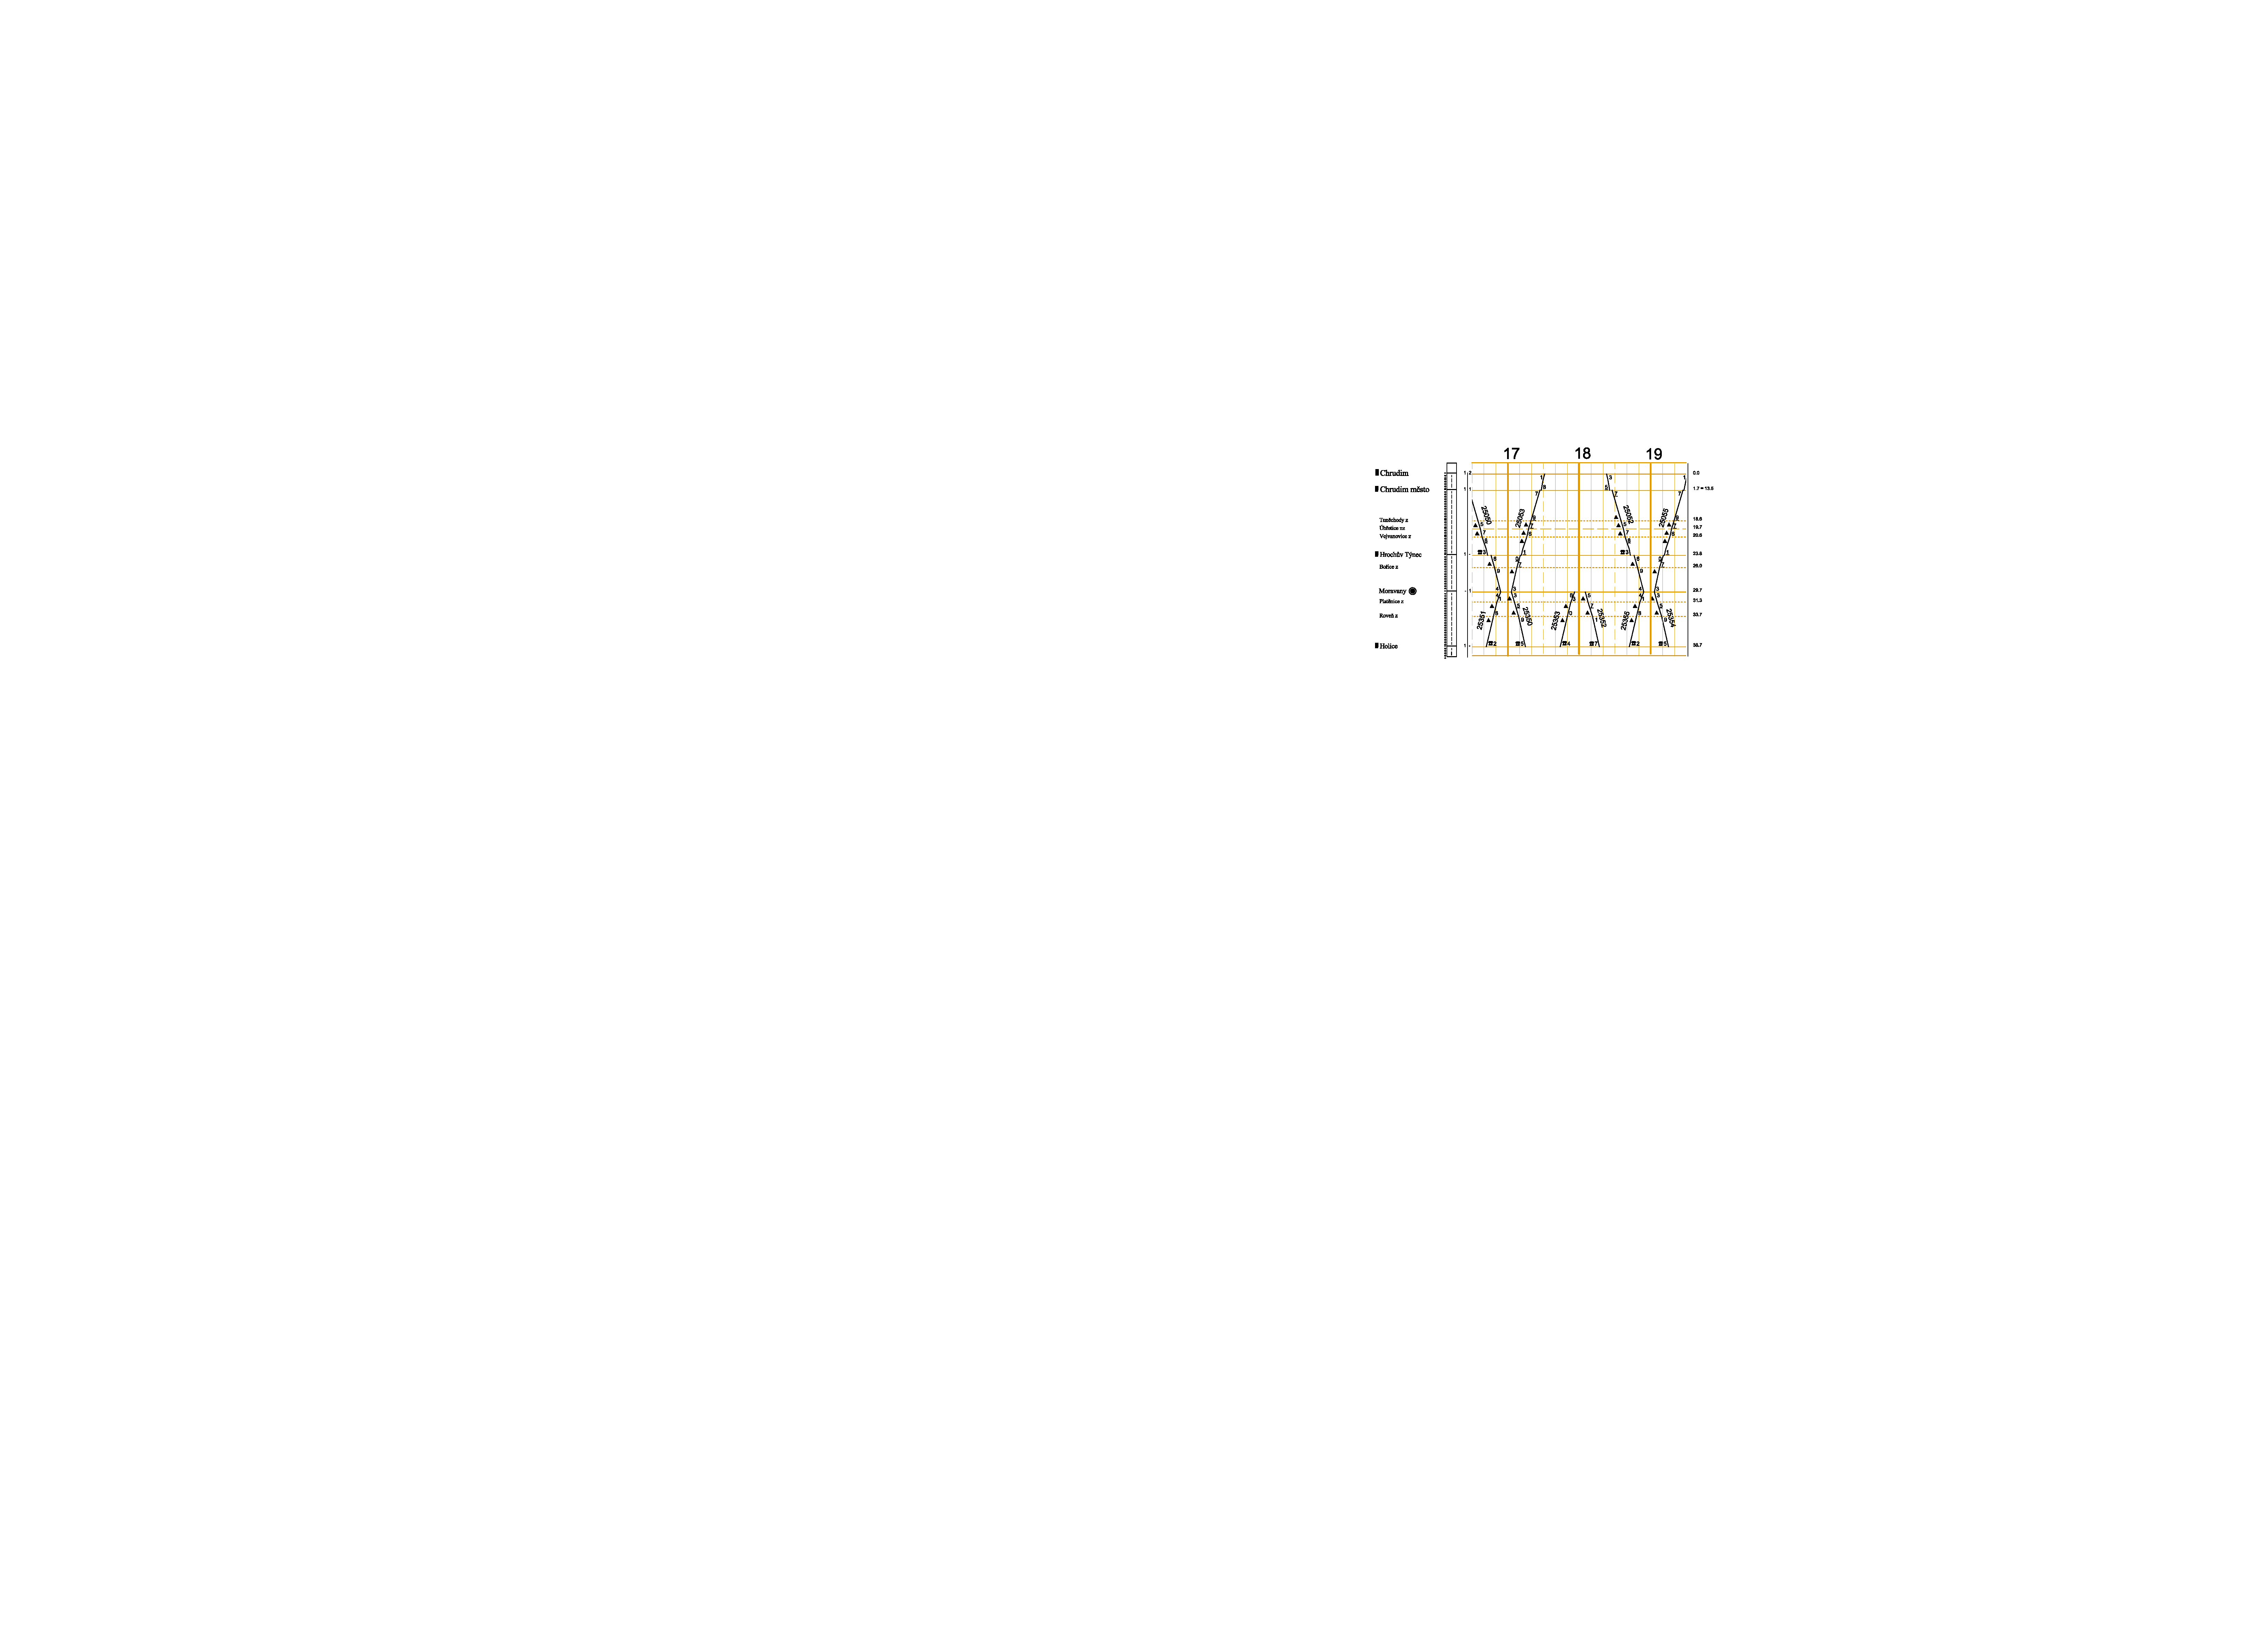
\includegraphics[width=\textwidth]{../img/kap1_uvod_grafikon}
	\caption{Příklad nákresného jízdního řádu}
	\label{fig:uvod:njr_bez_anotaci}
\end{figure}

Všichni zaměstnanci zúčastněni na provozu železniční dopravy potřebují mít přehled o~plánovaném i~aktuálním provozu v~traťových úsecích. Jelikož pro tuto potřebu reprezentovat data textovou formou není vhodné, využívá se znázornění průběhu jízd vlaků ve formátu, který se v~železniční dopravě označuje jako \textit{nákresný jízdní řád}. 
Existují aplikace, které s~nákresným jízdním řádem pracují. Aplikace se však často při jeho zobrazování potýkají s~problémy. Dále existují nástroje, které ke svému fungování nákresný jízdní řád nepotřebují, ale práce s~nimi by se mohla zlepšit, pokud budou nákresný jízdní řád zobrazovat. Chtěli bychom proto vytvořit nástroj, který bude nákresné jízdní řády zobrazovat a~umožní s~nimi co nejlépe pracovat. Hlavním cílem práce bude vytvořit takový nástroj jako grafickou komponentu integrovatelnou do různých aplikací.

Než ale blíže určíme, jaké konkrétní požadavky by měla tato grafická komponenta splňovat, podrobně si v~této kapitole nákresný jízdní řád představíme a~zvážíme jeho existující uplatnění i~možná využití. Jeho vlastnosti, které si budeme popisovat, jsou často specifické pro české prostředí.

\section{Nákresné jízdní řády}
\label{kap:uvod:nakresny_jizdni_rad}

Základem nákresného jízdního řádu je síť vodorovných a~svislých čar umístěná v~grafu, který je znázorněn na obrázku \ref{fig:uvod:njr_graf}. Svislou osou grafu je kilometrická poloha na trati. Vodorovná osa značí čas, kde čísla na obrázku představují celé hodiny.

\begin{figure}[ht]
	\centering
	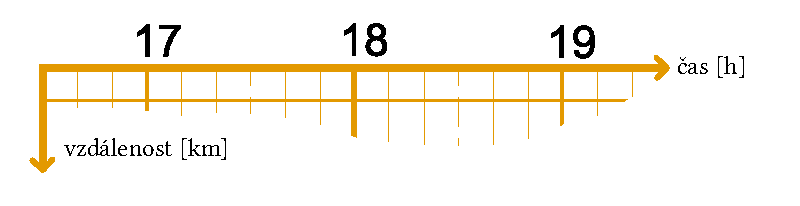
\includegraphics[width=0.7\textwidth]{../img/kap1_njr_graf}
	\caption{Osy nákresného jízdního řádu}
	\label{fig:uvod:njr_graf}
\end{figure}

Význam vodorovných a~svislých čar si vysvětlíme s~pomocí obrázku \ref{fig:uvod:njr_osy}, který obsahuje nákresný jízdní řád doplněný anotacemi ke zmíněným čarám.

Na trati se nachází významná místa (například stanice, zastávky nebo výhybny), které označujeme jako \textit{dopravní body}. Vodorovné čáry odpovídají dopravním bodům rozmístěných v~grafu podle jejich kilometrické polohy vzhledem k~trati. Na obrázku \ref{fig:uvod:njr_osy} pro přehlednost modře podbarvená plná čára reprezentuje stanici Chrudim. Přerušovaná čára podbarvená zelenou barvou patří nákladišti a~zastávce Úhřetice. Červeně podbarvená tečkovaná čára značí zastávku Bořetice. Vzor (nebo i~tloušťka) čáry tak určuje typ dopravního bodu.

Stejným způsobem se rozlišují svislé čáry značící časové údaje v~intervalech po deseti minutách. Plná čára na obrázku \ref{fig:uvod:njr_osy} označena 
\includegraphics[height=10.0pt]{../img/cas_osa_typ_1} je určena pro hodiny, 
\includegraphics[height=10.0pt]{../img/cas_osa_typ_2} pro půlhodiny a~tenká plná čára označená 
\includegraphics[height=10.0pt]{../img/cas_osa_typ_3} je určena pro jiné časové údaje.

\begin{figure}[ht]
	\centering
	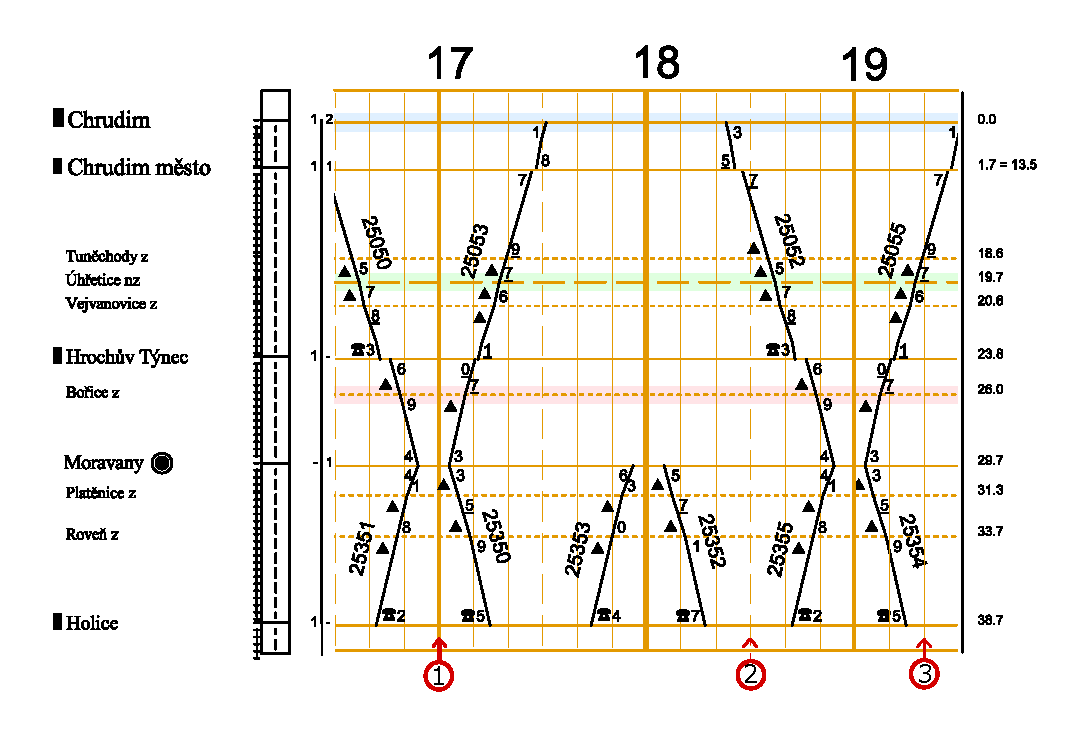
\includegraphics[width=\textwidth]{../img/kap1_uvod_grafikon_osy}
	\caption{Nákresný jízdní řád s~vyznačenými typy vodorovných a~svislých čar}
	\label{fig:uvod:njr_osy}
\end{figure}

\subsection*{Průběh jízdy vlaků v~nakresném jízdním řádu}
Popsaná síť vodorovných a~svislých čar je nutným základem pro vyobrazení nejdůležitějšího obsahu nákresného jízdního řádu, kterým jsou průběhy jízd vlaků. Pomocí obrázku \ref{fig:uvod:njr_vlaky} obsahující zvýrazněné průběhy jízd některých vlaků si popíšeme princip jejich vyobrazování.

\begin{figure}[ht]
	\centering
	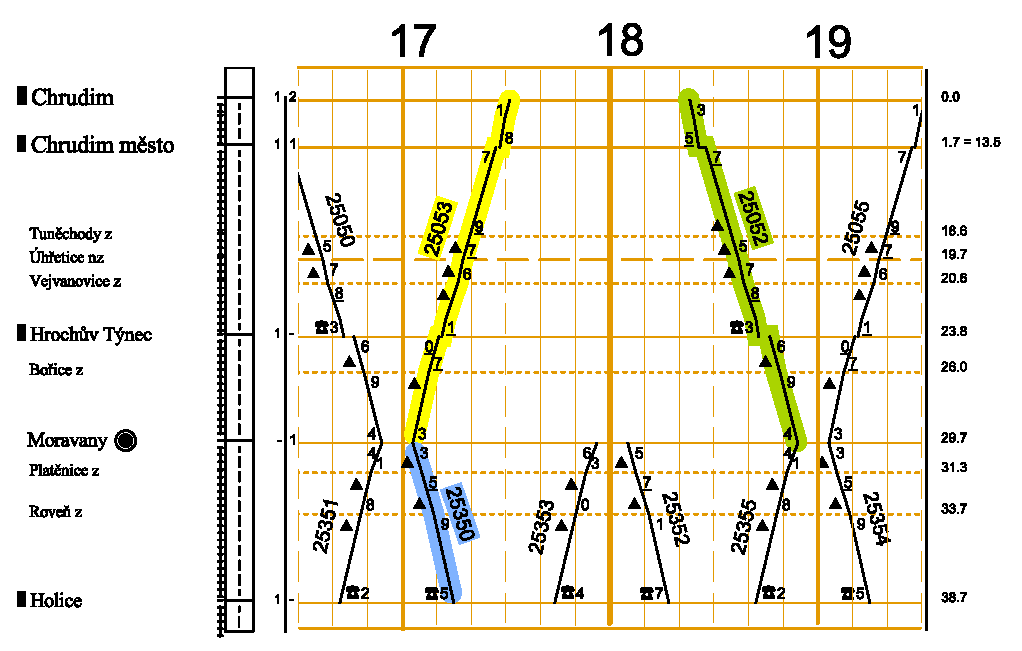
\includegraphics[width=\textwidth]{../img/kap1_uvod_grafikon_vlaky}
	\caption{Nákresný jízdní řád s~vyznačenými průběhy jízd vlaků 25350, 25052 a~25053}
	\label{fig:uvod:njr_vlaky}
\end{figure}

Na obrázku \ref{fig:uvod:njr_vlaky} se nachází vlak označený číslem 25053 se žlutě podbarvenou šikmou čarou reprezentující průběh jeho jízdy. Všimněme si, že tato čára tvoří průsečíky s~vodorovnými čarami reprezentující dopravní body. Takový průsečík pak představuje příjezd, odjezd nebo průjezd vlaku dopravním bodem v~čase, který odpovídá pozici průsečíku na časové ose. Průsečík šikmé čáry, který se vyskytne na časové ose jako první, patří k~dopravnímu bodu, ze kterého vlak vyjíždí. Poslední průsečík naopak odpovídá dopravnímu bodu, kde jízda vlaku končí. V~případě vlaku 25053 vlak vyjíždí přibližně v~sedmnáct hodin ze stanice Moravany a~jede směrem na Chrudim, do které dojede kolem půl šesté. Tímto popsaným principem můžeme sledovat celý průjezd vlaku tratí v~závislosti na čase a~jeho poloze.

Podobně je možné z~obrázku \ref{fig:uvod:njr_vlaky} určit průběh jízdy i~u~ostatních vlaků. Zeleně podbarvená lomená čára představuje průběh jízdy vlaku 25052, který jede v~opačném směru do Moravan. Modře podbarvený vlak 25350 odjíždí z~Moravan ve stejný čas jako vlak 25053, ale v~opačném směru na Holice. Svislé čáry těchto dvou vlaků, které jsou vizuálně spojeny v~Moravanech, od sebe můžeme odlišit pochopením faktu, že kdybychom je vnímaly jako celek zobrazující průběh jízdy jednoho vlaku, záznam by vzhledem k~časové ose nedával smysl, jelikož by se vracel do minulosti.

\pagebreak

Nezbytnou součástí vyobrazení informací o~jízdě vlaků v~nákresném jízdním řádu je vhodně umístěné číslo vlaku v~blízkosti šikmé čáry, která odpovídá průběhu jeho jízdy. Podle pravidel provozu na českých železničních tratích má každý vlak přiděleno unikátní číslo. Číslo je v~nákresném jízdním řádu umístěno způsobem, z~kterého je zřejmé, k~jakému vlaku patří. Číslo se umisťuje v~blízkosti šikmé čáry vlaku tak, aby směr čtení čísla odpovídal směru jízdy. Šikmá čára je pak pomyslným řádkem, na kterém je číslo napsáno.

\subsubsection*{Výhody zobrazování průběhu jízd vlaků nákresným jízdním řádem}

Abychom pochopili, v~jakých situacích je možné nákresné jízdní řády používat, popíšeme si výhody, které přináší oproti jiným formám jízdního řádu. Z~nákresného jízdního řádu je lehké zjistit, jak jsou úseky mezi dopravními body obsazeny jízdami vlaků. Drážní zaměstnanec tak má přehled o~dopravní situaci na celé trati.

Vedle nákresných jízdních řádů existují jízdní řády v~textové formě, které jsou užitečné například pro cestující, ale nemůžou nahradit roli nákresného jízdního řádu. Jedním z~textových formátů zobrazující informace o~jízdě vlaků je knižní jízdní řád, jehož výřez je uvedený na obrázku \ref{fig:uvod:kjr}. Můžeme vidět, že informace v~něm obsažené jsou vztaženy k~jen konkrétnímu vlaku a~těžko se mezi sloupečky, obsahující plány jízd vlaků, dají hledat hlubší souvislosti. Pro porovnání jsou vlaky z~výřezu knižního jízdního řádu vyobrazeny na nákresném jízdním řádu na obrázku \ref{fig:uvod:njr_vyrez}.

\begin{figure}[ht]
	\centering
	\includegraphics[width=\textwidth]{../img/kap1_uvod_grafikon_kjr_vyrez}
	\caption{Nákresný jízdní řád s~podbarvenými průběhy jízd vlaků z~knižního jízdního řádu na obrázku \ref{fig:uvod:kjr}}
	\label{fig:uvod:njr_vyrez}
\end{figure}

\begin{figure}[ht]
	\centering
	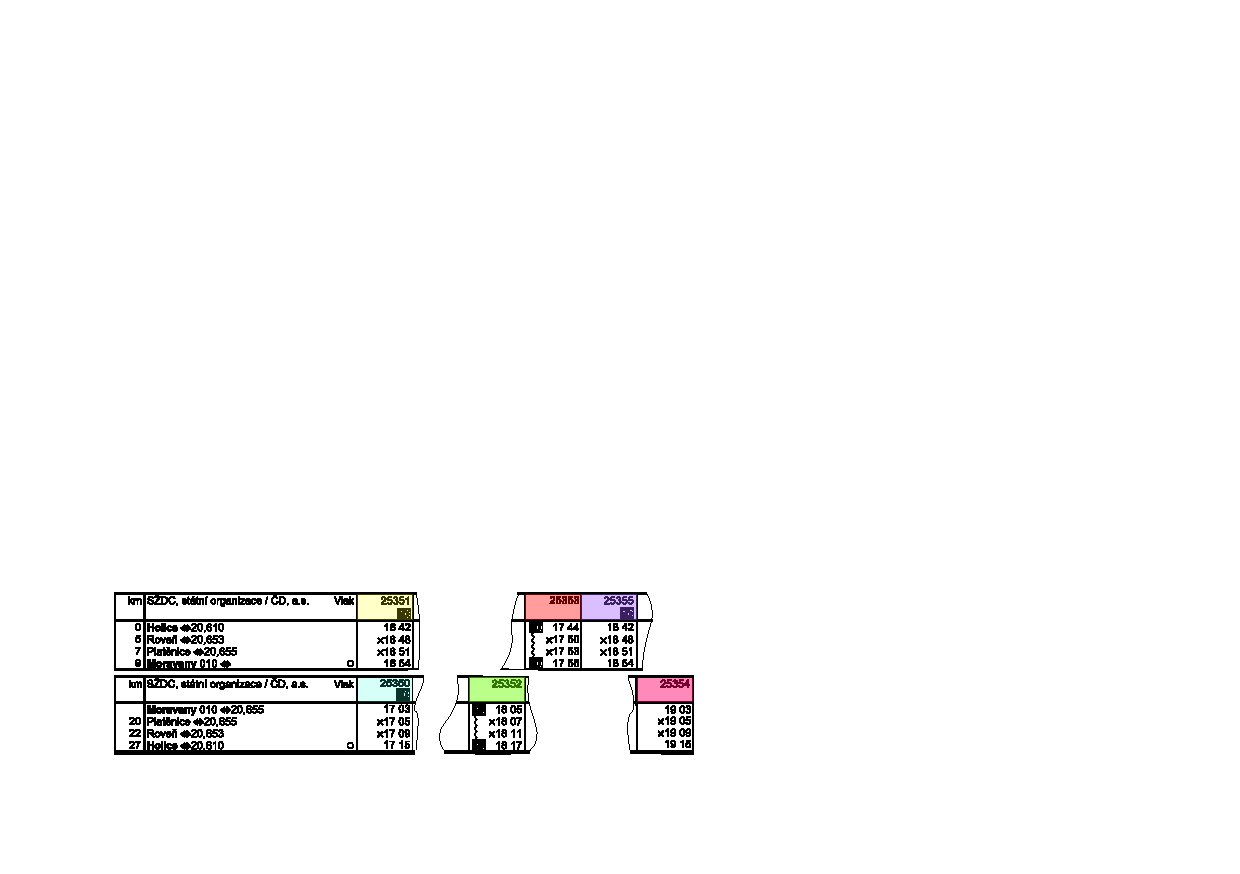
\includegraphics[width=0.9\textwidth]{../img/kap1_kjr_moravany_holice_vyrez}
	\caption{Výřez z~knižního jízdního řádu se zvýrazněnými čísly vlaků odpovídající podbarveným průběhům jízd těchto vlaků na obrázku \ref{fig:uvod:njr_vyrez}}
	\label{fig:uvod:kjr}
\end{figure}

V~další části si popíšeme, jak z~nákresného jízdního řádu můžeme vyčíst přesné časy příjezdů a~odjezdů obsažených ve sloupcích knižních jízdních řádů.

\subsection*{Informace k~jízdě vlaků v~nákresném jízdním řádu}
\label{kap1:koty_a_informace_o_prubehu_vlaku}
Ještě jsme si neuvedli, jak v~nákresných jízdních řádech určit přesný čas příjezdů, odjezdů a~průjezdů vlaku dopravními body. Tyto informace se nachází v~ostrých úhlech, které dopravní body s~trasami vlaků svírají, a~nazývají se \textit{kóty}. V~kótách se pouze uvádí jednotky minut, například pro čas 19:15 se uvede 5. Na obrázku \ref{fig:uvod:koty} můžeme vidět, jak jsou tímto způsobem ve výřezu nákresného jízdního řádu zaznamenány časy odjezdů (a~příjezdu do Holic) z~knižního jízdního řádu.

\begin{figure}[ht]
	\centering
	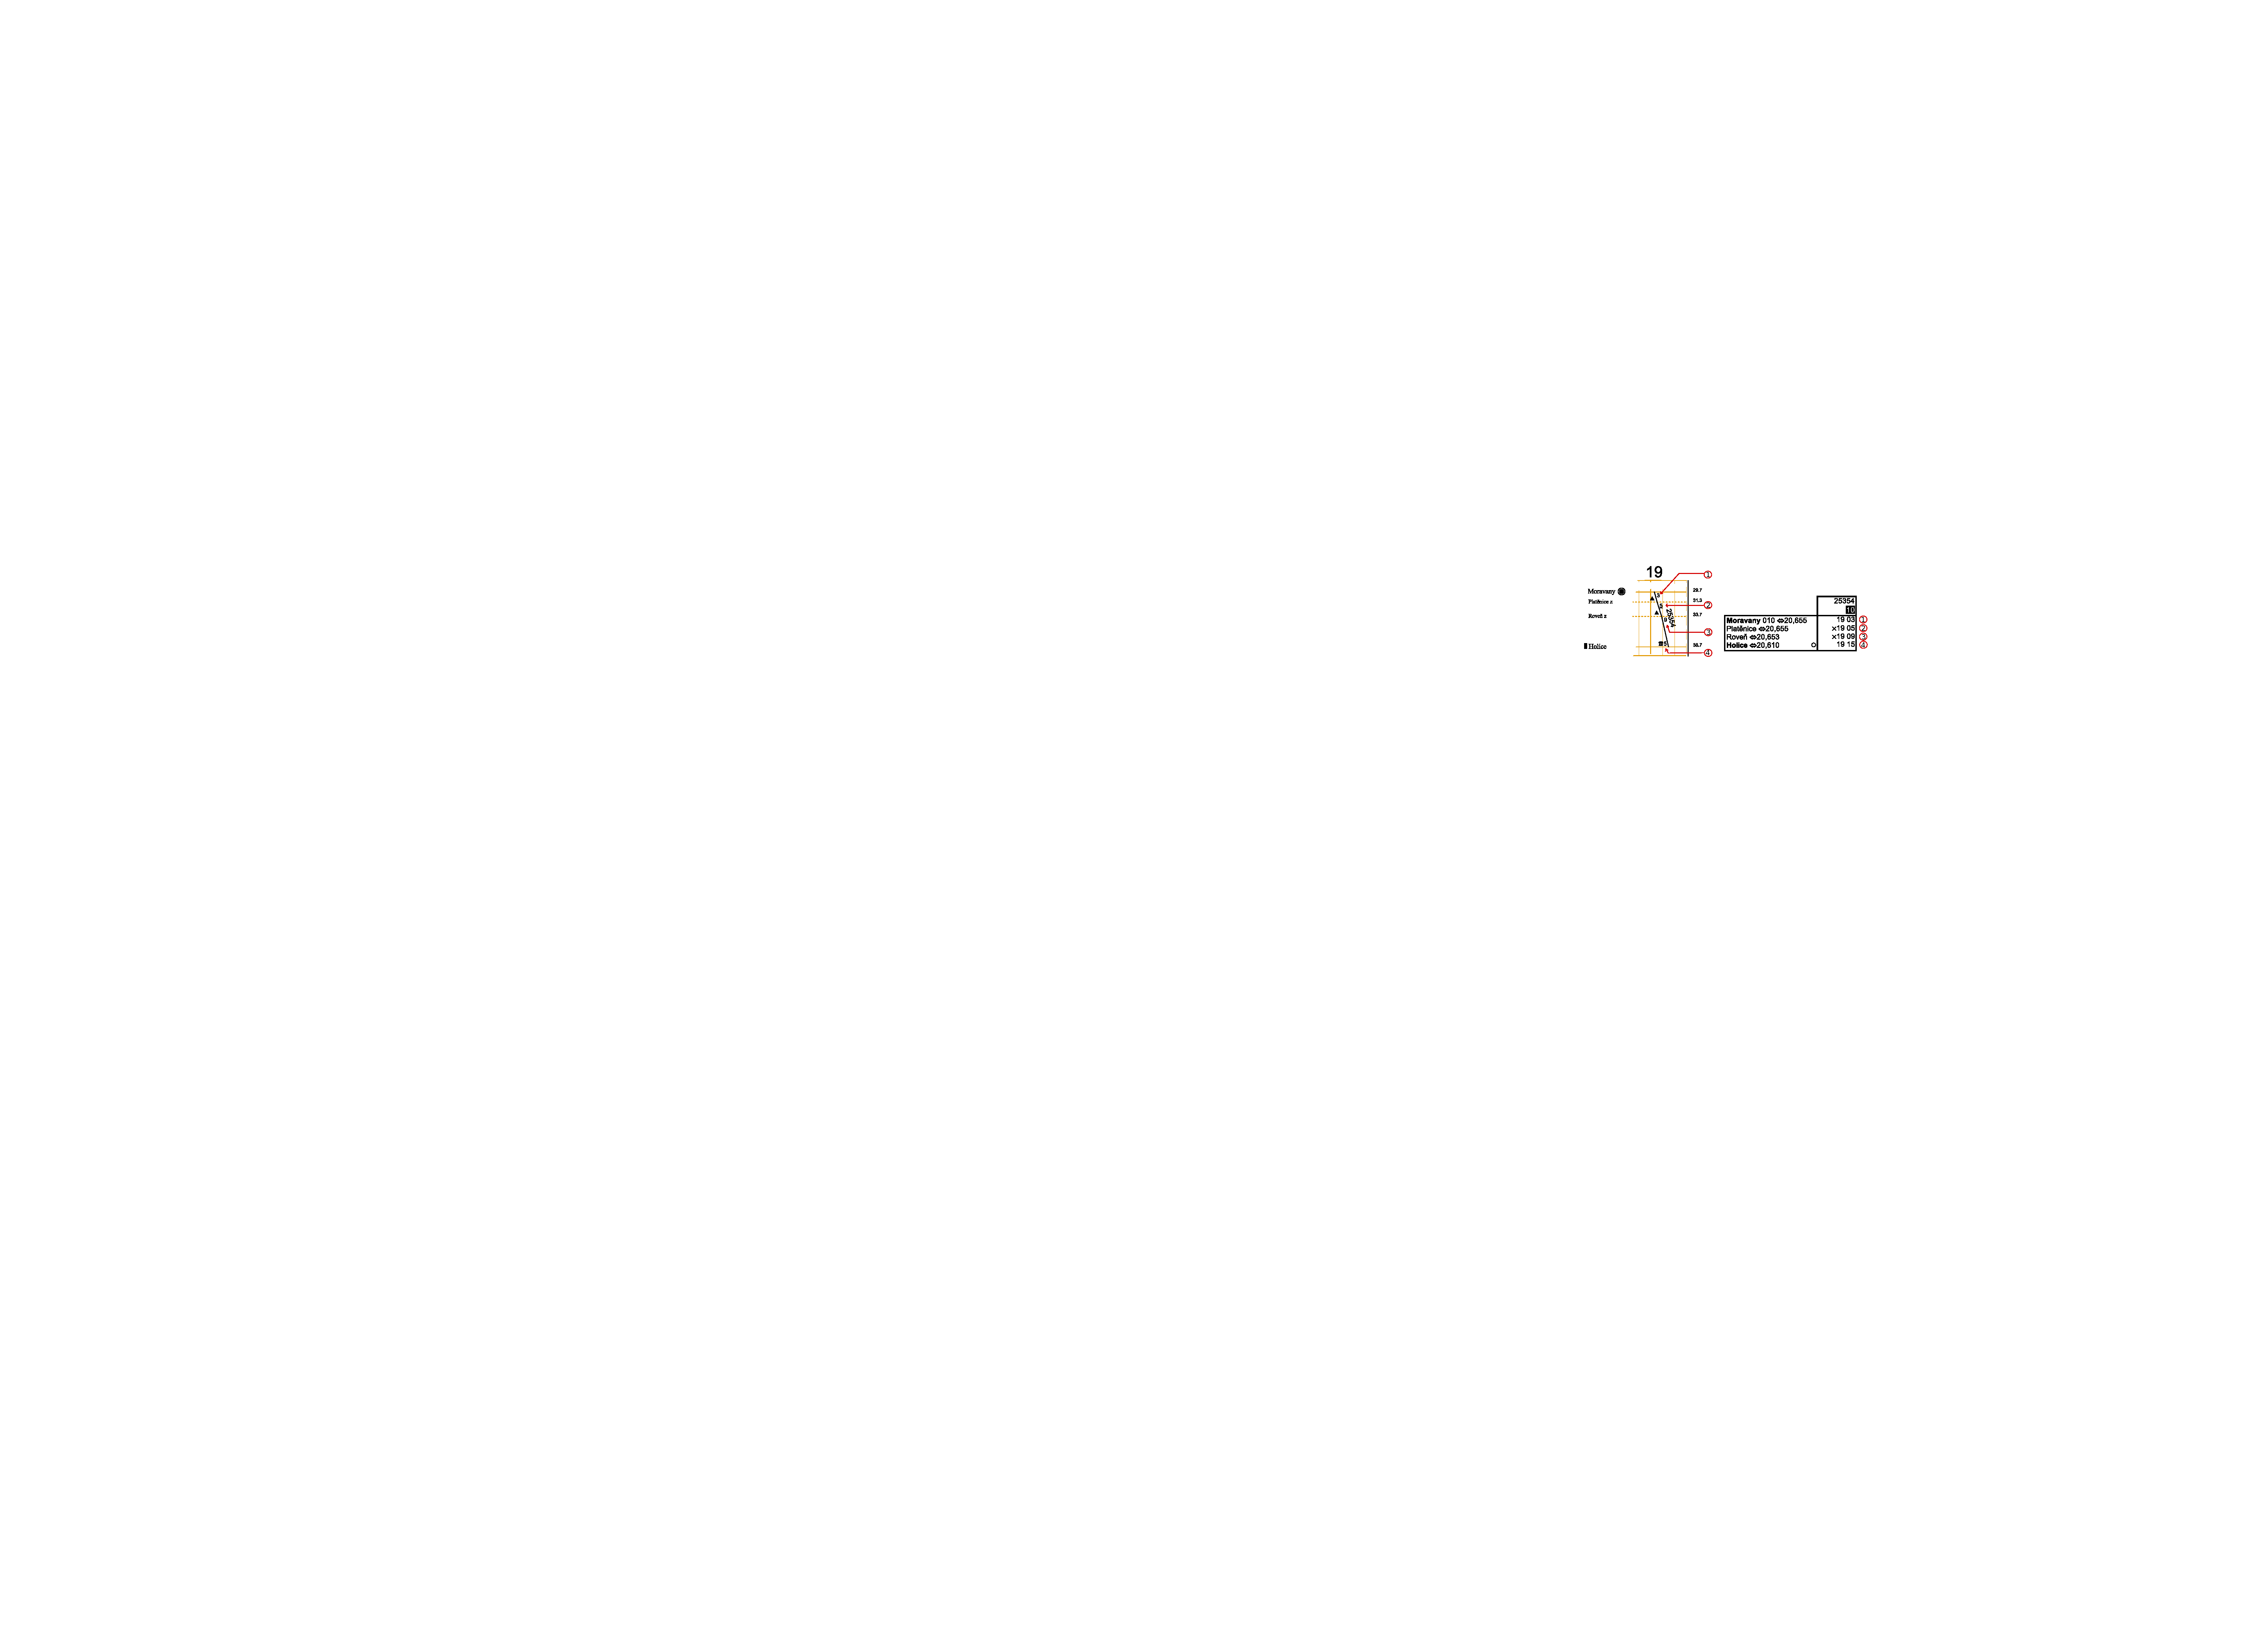
\includegraphics[width=\textwidth]{../img/kap1_koty_popis}
	\caption{Označené kóty v~nákresném jízdním řádu odpovídající časům v~knižním jízdním řádu}
	\label{fig:uvod:koty}
\end{figure}

Ostré úhly neslouží pouze k~umisťování kót, ale je možné do nich přidat i~další informace, které by se musely jinak složitě hledat jinde. Navíc se někdy zobrazení kót mění. Příklady zmiňovaných informací a~změn se nachází na obrázku \ref{fig:uvod:koty_dalsi}:

\begin{enumerate}[label=(\alph*)]
\item Ikona telefonu značí ohlašovací povinnost strojvedoucího při příjezdu do dopravního bodu.
\item Pokud má vlak v~dopravním bodu dobu pobytu kratší než půl minuty a~nejedná se o~průjezd, kóta příjezdu se nahradí trojúhelníkem.
\item Podtržená kóta značí o~půlminuty více. Na obrázku vlak odjíždí z~dopravního bodu mezi pěti minutami a~30 sekundami až šesti minutami, vhledem k~používanému zaokrouhlení času pro kóty.
\end{enumerate}

\begin{figure}[ht]
    \centering
    \begin{subfigure}[b]{0.3\textwidth}
        
\includegraphics[width=0.7\textwidth]{../img/koty_dalsi_set_x}
        \caption{Ohlašovací povinnost nařízena}
    \end{subfigure}
    \begin{subfigure}[b]{0.3\textwidth}
        
\includegraphics[width=0.7\textwidth]{../img/koty_dalsi_set_y}
        \caption{Pobyt kratší než půl minuty}
    \end{subfigure}
    \begin{subfigure}[b]{0.3\textwidth}
        
\includegraphics[width=0.7\textwidth]{../img/koty_dalsi_set_z}
        \caption{Odjezd o~půl minuty později}
    \end{subfigure}
    \caption{Další informace umístitelné do ostrých úhlů}
    \label{fig:uvod:koty_dalsi}    
\end{figure}

\newpage
\subsection*{Další informace zobrazované v~nákresných jízdních řádech}
\label{kap1:dalsi_info}
Doposud jsme si popisovali, jak se zobrazují informace související s~jízdou vlaku. Nákresný jízdní řád se ale nemusí omezovat pouze na tyto informace. Na obrázku \ref{fig:uvod:njr_doplnky} můžeme vidět několik sloupců. Zeleně podbarvený sloupec obsahuje názvy dopravních bodů, umístěných podle kilometrické vzdálenosti na trati. V~blízkosti názvů se pak nachází značení, přidávající další informace o~dopravním bodu. Ve fialově podbarveném sloupci se nachází informace o~zabezpečení traťového úseku. Oranžově podbarvený sloupec zobrazuje kilometrické vzdálenosti dopravních bodů na trati.

\begin{figure}[ht]
	\centering
	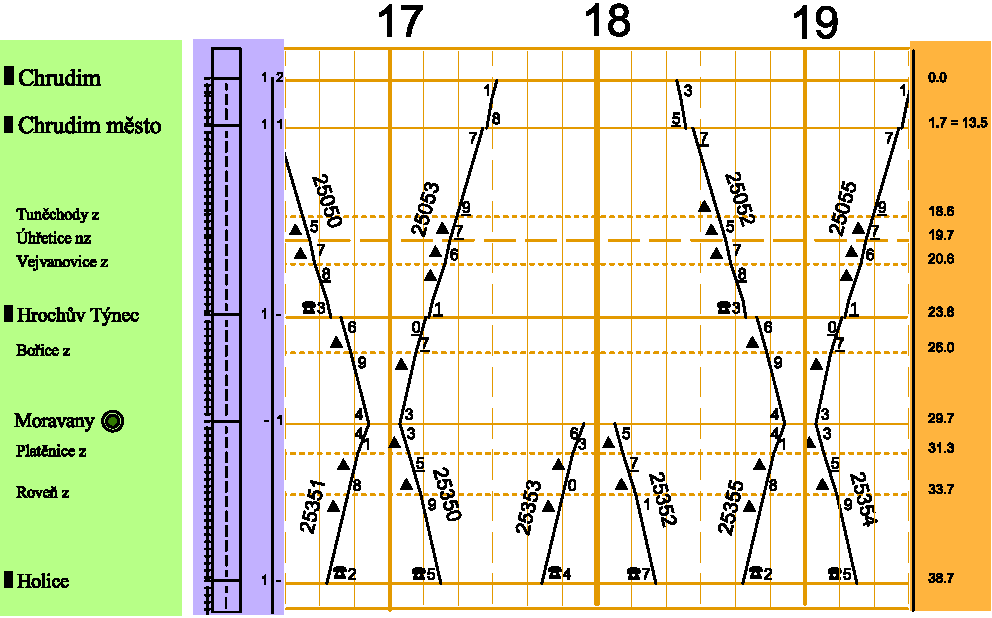
\includegraphics[width=0.85\textwidth]{../img/kap1_uvod_grafikon_doplnky}
	\caption{Nákresný jízdní řád s~podbarvenými sloupci nesoucí další informace}
	\label{fig:uvod:njr_doplnky}
\end{figure}

Tímto jsme dokončili popis všech informací v~nákresném jízdním řádu, poprvé uvedeném na obrázku \ref{fig:uvod:njr_bez_anotaci}.

\subsection*{Další typy nákresných jízdních řádů}
Až do této chvíle jsme si pro lehčí pochopení ukazovali pouze jeden typ nákresného jízdního řádu. Existuje ale více typů nákresných jízdních řádů. Nákresný jízdní řád na obrázku \ref{fig:uvod:slovensky_njr} se používá pro organizaci železniční dopravy na Slovensku a~jeho vizualizace se řídí doposud uvedenými pravidly, pouze se liší v~drobnostech, kterými jsou použité barvy nebo vzor čar.

\begin{figure}[ht]
	\centering
	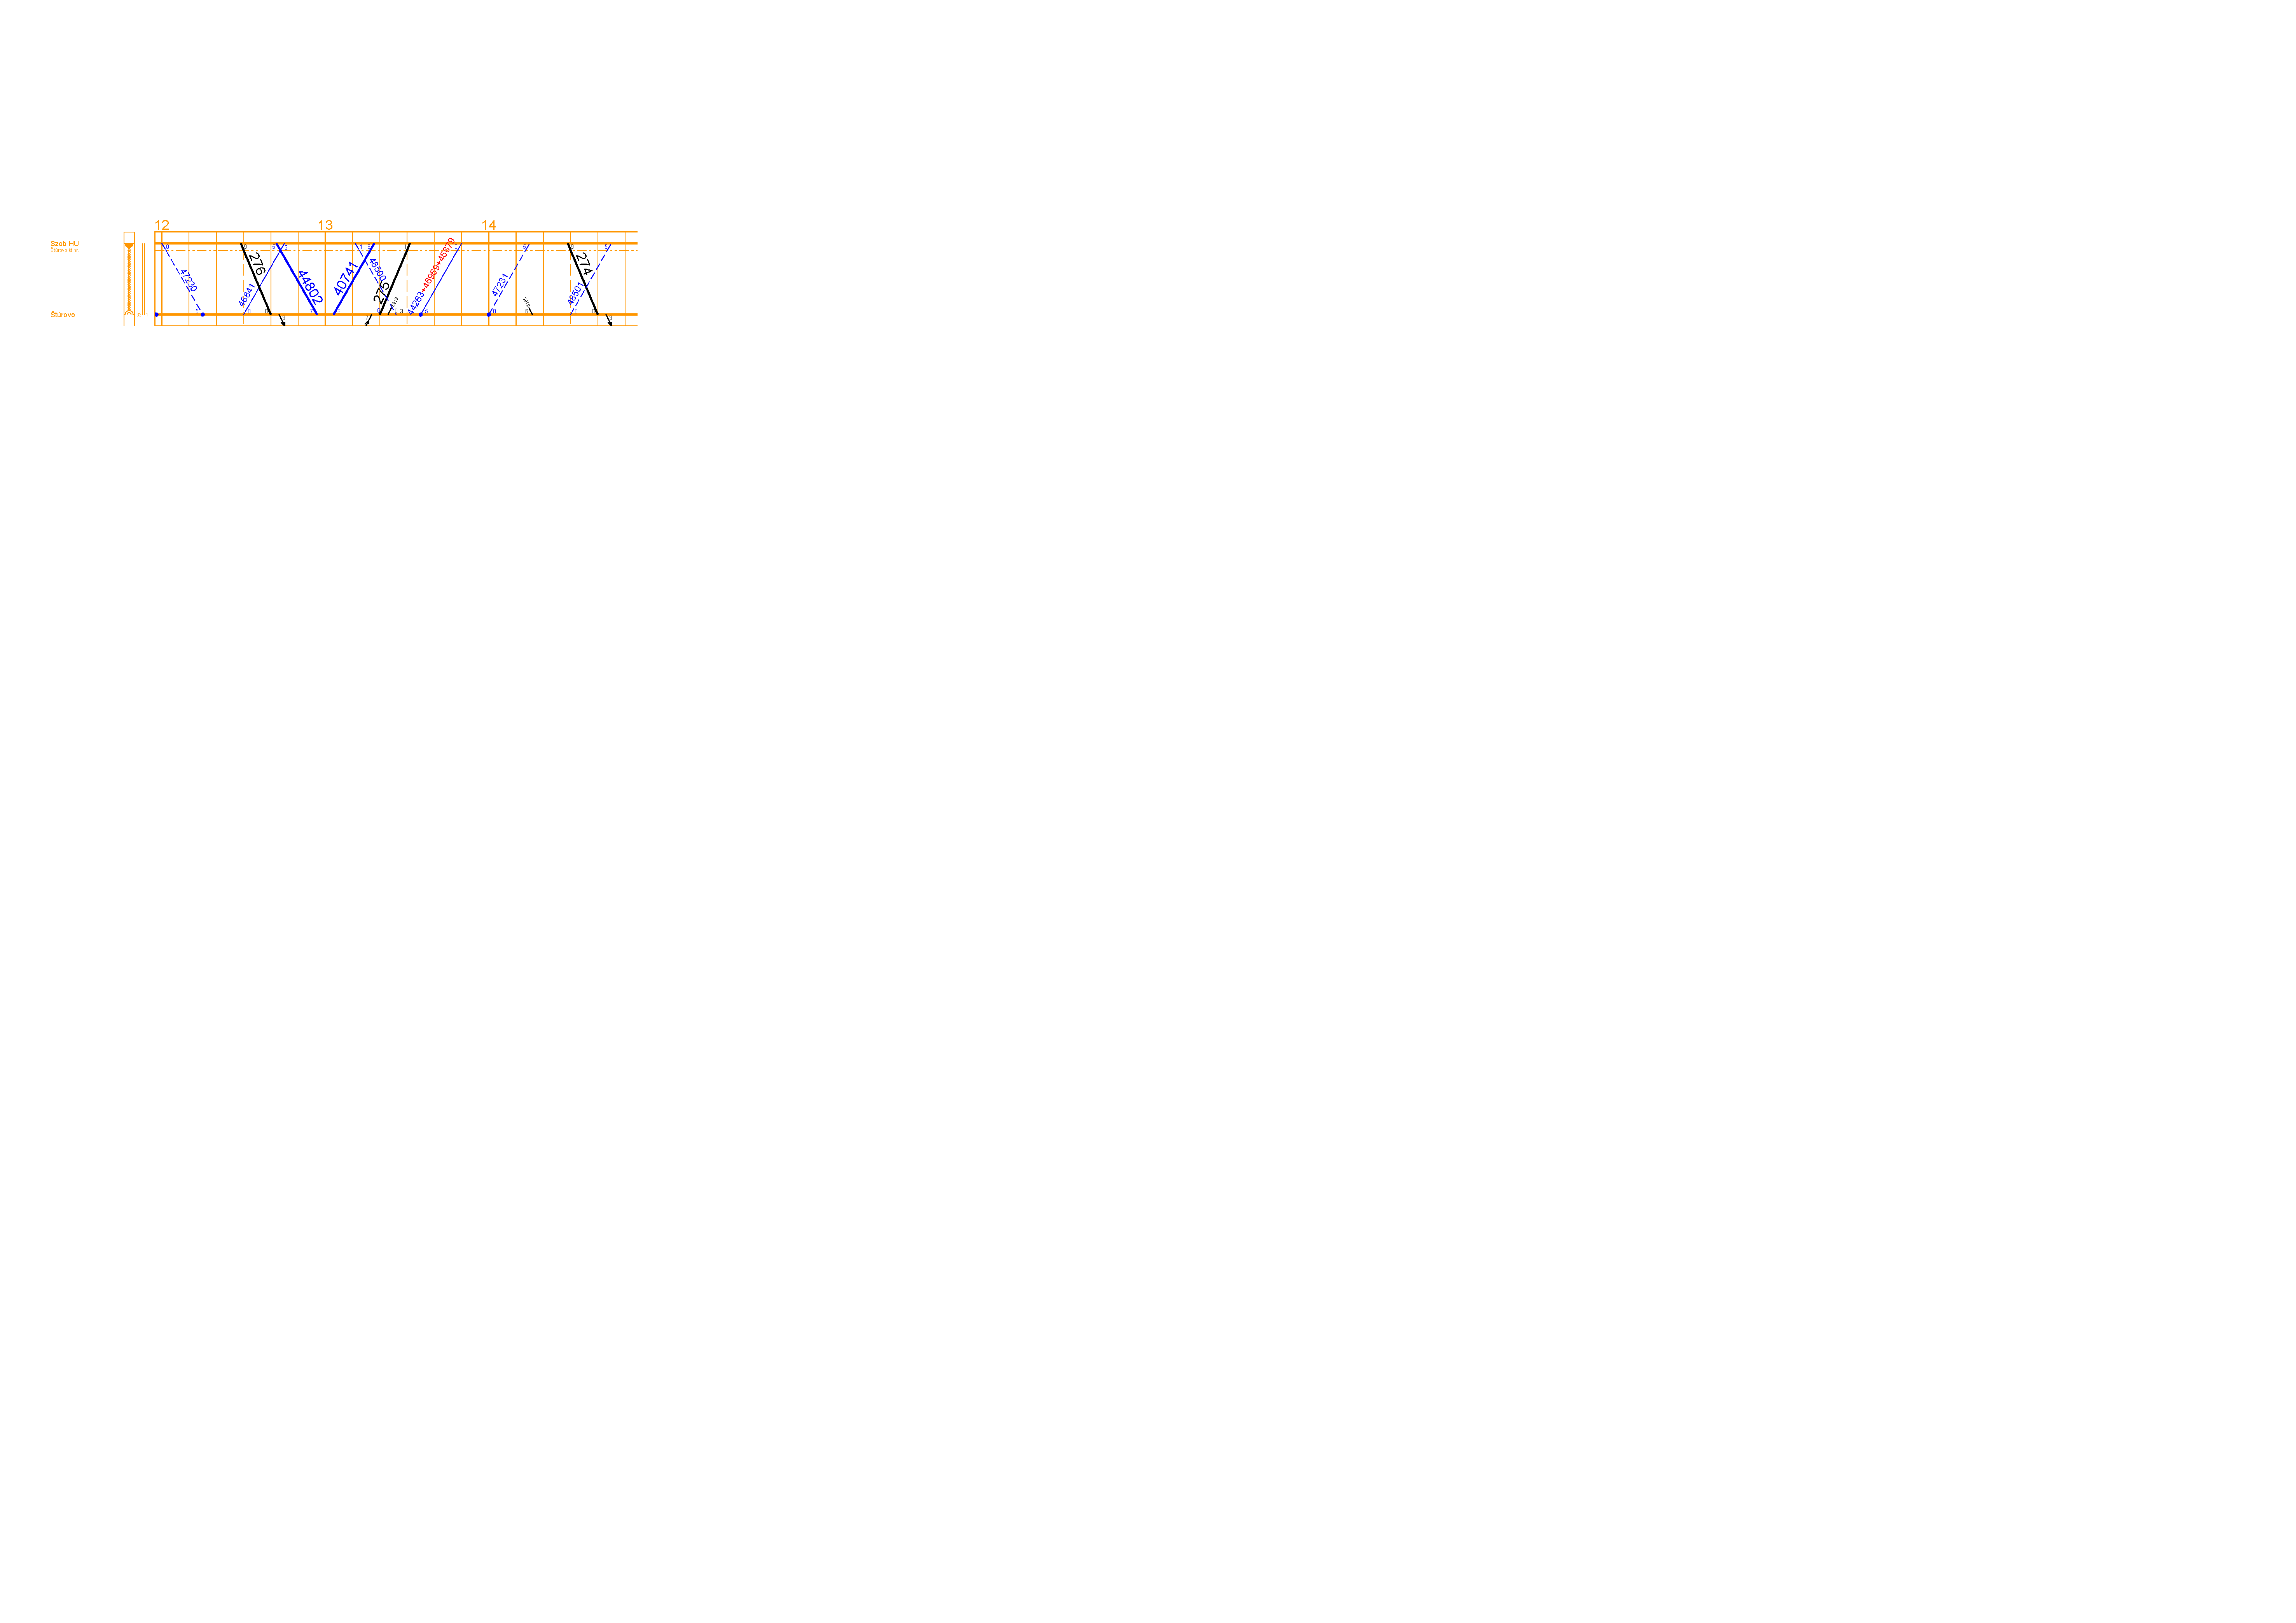
\includegraphics[width=\textwidth]{../img/kap1_slovensko}
	\caption{Další typ nákresného jízdního řádu}
	\label{fig:uvod:slovensky_njr}
\end{figure}
\newpage
Než si ale detailně uvedeme jiné typy nákresných jízdních řádů, které budou obvykle součástí různých aplikací, zasadíme je do kontextu grafikonu vlakové dopravy, s~kterým tyto aplikace pracují.

\section{Grafikon vlakové dopravy}
V~železniční dopravě se pracuje s~pojmem grafikon vlakové dopravy. Ten je v~přeneseném významu jiným označením pro zobrazení jízdy vlaků v~nákresném jízdním řádu. Proto se někdy nákresné jízdní řády označují jako listy grafikonu vlakové dopravy. Původně ale tento pojem představuje označení pro soubor předpisů a~pomůcek určených k~plánování vlakové dopravy. Na základě mnoha často protichůdných požadavků se pomocí předpisů a~pravidel grafikonu vlakové dopravy sestaví plán, sloužící jako předloha a~dokumentace, na kterou je se potřeba při organizaci dopravy a~řešení konfliktů vznikajících při provozu odkazovat. Takto sestavený plán je obsažen v~pomůckách grafikonu vlakové dopravy, mezi které patří právě listy nákresného jízdního řádu nebo jízdní řády pro cestující. Provoz v~české železniční síti je pod správou státní organizace Správa železniční dopravní cesty, která pro každý rok sestavuje nový grafikon vlakové dopravy. Dokumentem popisující tento proces je Směrnice SŽDC č. 69 pro tvorbu jízdního řádu a~pomůcek GVD\footnote{grafikon vlakové dopravy}. Naše práce se problematice sestavování grafikonu vlakové dopravy věnovat nebude, více se o~ní může čtenář dozvědět v~knize Železniční doprava, Gašparík a~Kolář \cite{zel_doprava}.

\section{Práce s~grafikony vlakové dopravy}
\label{aplikace_gvd}
V~této části se seznámíme s~dalšími typy nákresných jízdních řádů. Pokud budeme mluvit o~práci s~grafikonem vlakové dopravy, budeme tímto spojením označovat činnost, která je založena na používání pravidel a~pomůcek grafikonu vlakové dopravy -- asi nejznámější činností je řízení provozu na železnici. Abychom věděli, jak může být námi vytvářený nástroj používán, představíme si jeho možná využití při práci s~grafikonem vlakové dopravy.

\subsection*{Aplikace pro vlakovou dopravu}
\label{prace_gvd}
Organizace vlakové dopravy se v~české železniční síti až do vybudování infrastruktury výpočetní techniky odehrávala pouze na papíře. V~současnosti existují aplikace pracující s~grafikonem vlakové dopravy nasazené v~reálném provozu, které mají pozitivní dopad na organizaci i~zabezpečení provozu na trati. Některé takové aplikace si v~této části popíšeme. Nové aplikace, používající námi vytvářenou grafickou komponentu zobrazující nákresný jízdní řád, se pak většinou budou snažit chování nyní uvedených aplikací napodobit.

\newpage
\subsubsection*{Aplikace GTN}
Aplikace GTN\footnote{Graficko-technologická nadstavba} společnosti AŽD Praha zobrazuje uskutečněnou a~výhledovou (budoucí) dopravu. Zachycuje tak současnou situaci na trati. Okno aplikace s~komponentou zobrazující nákresný jízdní řád se nachází na obrázku \ref{fig:gtn_okno}. V~aplikaci je možné plánovat výhledovou dopravu úpravou průběhu jízd vlaků přímo v~komponentě. Upravovaný vlak je navíc od ostatních vizuálně rozlišitelný hnědou barvou a~zvětšenými kótami. Komponenta může zobrazit současnou dopravu v~různých časových intervalech. Aplikace tak nezobrazuje nákresný jízdní řád, jehož obsah by byl neměnný, ale rozšiřuje ho o~prvky, které z~komponenty zobrazující nákresný jízdní řád vytváří interaktivní nástroj pro práci s~grafikonem vlakové dopravy. Pokud by si chtěl čtenář práci s~aplikací vyzkoušet, existuje volně přístupná demoverze \cite{GTN_demoverze} aplikace.

\begin{figure}[!htb]
	\centering
	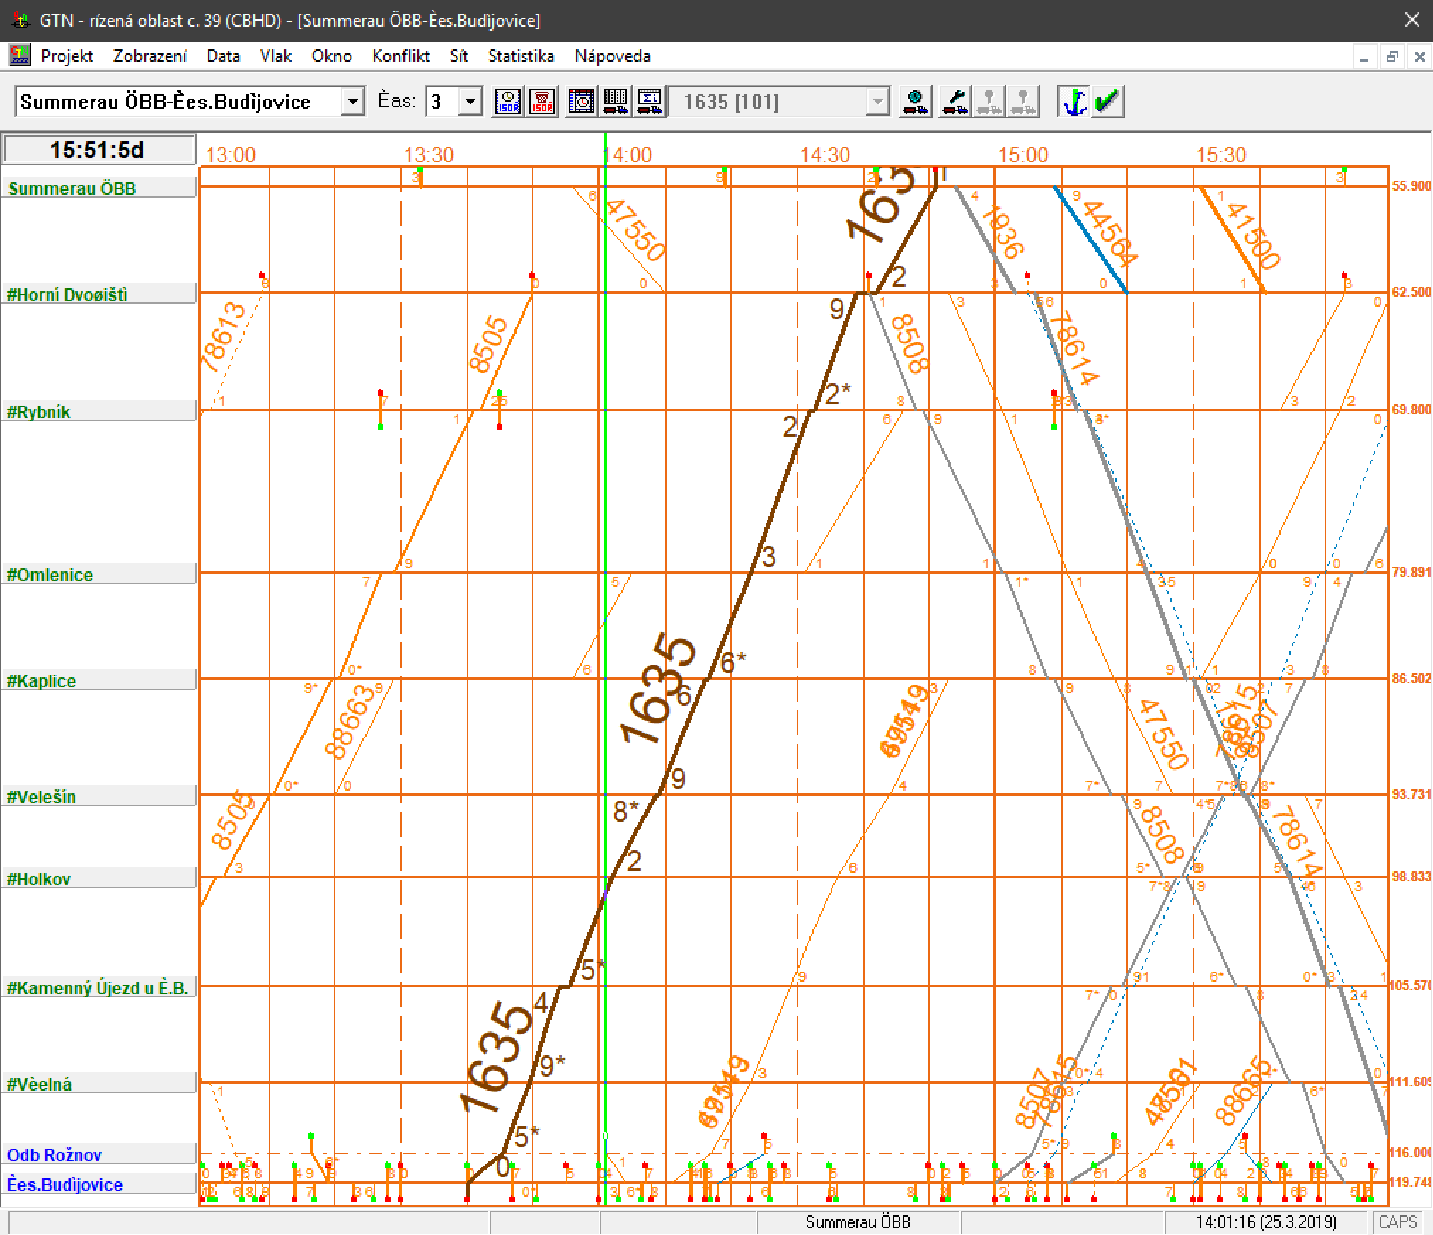
\includegraphics[width=0.75\textwidth]{../img/kap1_gtn_okno_interval_3h}
	\caption{Okno aplikace GTN}
	\label{fig:gtn_okno}
\end{figure}

\subsubsection*{Aplikace v~rámci IS ISOR CDS}
Aplikace pro práci s~grafikonem vlakové dopravy nabízena v~rámci informačního systému ISOR CDS \cite{ISOR_CDS} od OLTIS Group je zaměřena stejně jako aplikace GTN na prohlížení současného provozu. Na obrázku \ref{fig:oltis_window} můžeme vidět, jak aplikace vizualizuje nákresný jízdní řád. Všimněme si, že narozdíl od doposud popisovaného chování nezobrazuje dopravní body na vertikální ose podle jejich kilometrické polohy, ale rozmisťuje je rovnoměrně pro jednodušší zobrazení nákresného jízdního řádu. Taková změna v~zobrazení není nijak závadná, ačkoliv porušuje námi popsané zásady pro zobrazení nákresného jízdního řádu. V dalších částech práce budeme narážet na podobné odchylky, nikdy ale zásadně neporuší popsané rozpoložení uvedené na začátku kapitoly.
Na pravé hraně grafické komponenty zobrazující nákresný jízdní řád nabízí aplikace posuvník pro změnu zobrazené části traťového úseku. Stejným způsobem umožňuje na horizontále výběr zobrazovaného časového intervalu. Obě dvě aplikace tedy nabízí podobné možnosti při zobrazování nákresného jízdního řádu, volí jen jiný způsob ovládání.

\begin{figure}[ht]
	\centering
	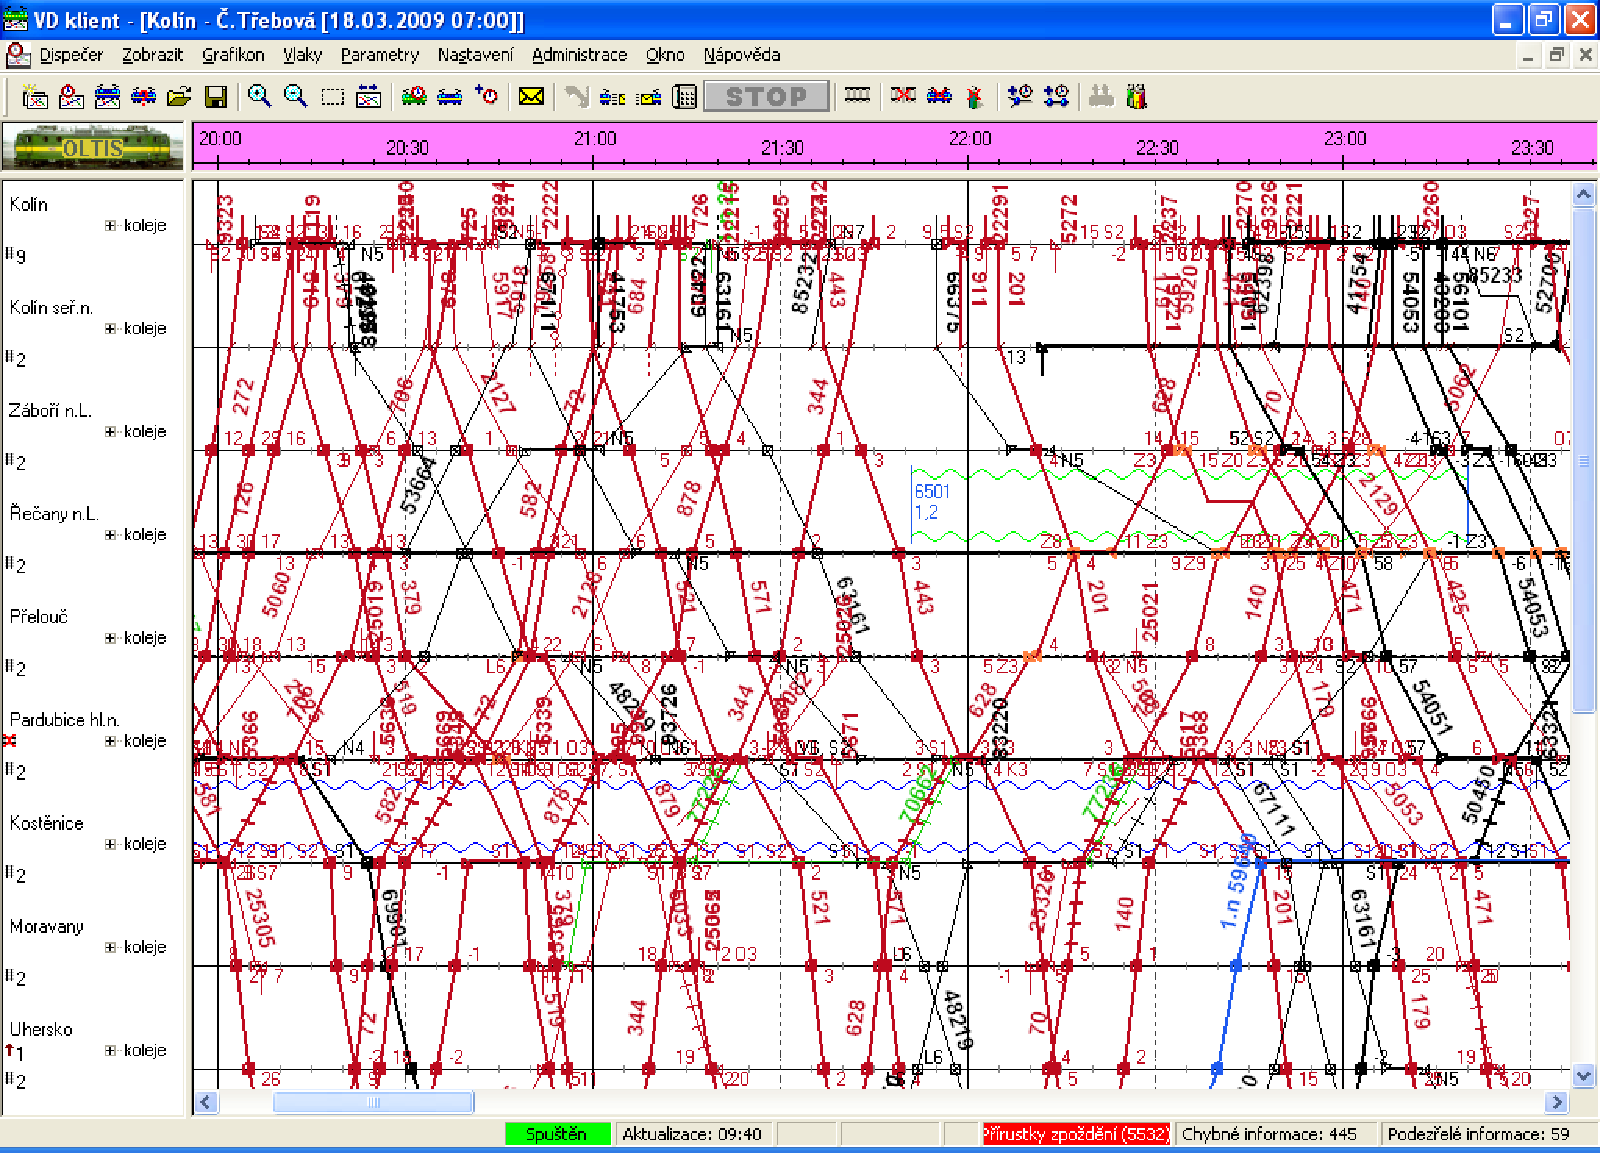
\includegraphics[width=0.9\textwidth]{../img/kap1_ISOR_window}
	\caption{Aplikace Grafikon od OLTIS Group, převzato ze stránky společnosti~\cite{ISOR_CDS}}
	\label{fig:oltis_window}
\end{figure}

\subsection*{Grafikon vlakové dopravy mimo skutečný provoz}
\label{model_gvd}
V~následující části zjistíme, že námi vytvářená grafická komponenta zobrazující nákresný jízdní řád může být součástí aplikací, které nejsou určeny pro nasazení v~reálném provozu. Grafikon vlakové dopravy se zobrazeným nákresným jízdním řádem se nabízí použít i~v~jiných scénářích, zejména pak při aktivitách, které se snaží provoz na železnici simulovat.

\subsubsection{Vytváření studií pro vlakovou dopravu}
Nejblíže problémům vlakové dopravy řešených ve skutečné situaci jsou studie a~koncepty věnující se provozu na železnici, které k~prezentování svých výsledků využívají koncepčně sestavený grafikon vlakové dopravy a~nákresné jízdní řády. Tyto studie jsou většinou zpracovávány v~rámci různých bakalářských a~diplomových prací studentů dopravních fakult. Existují komerční nástroje, které jsou k~těmto účelům určené a~na základě zadaných dat můžou autorům pomoci se sestavením grafikonu vlakové dopravy a~vytvořením jeho pomůcek. Typickým řešením je pro fakultu koupit licenci takového nástroje. Jedním z~těchto nástrojů je FBS-Bahn \cite{FBS_BAHN}. Tímto nástrojem byl vytvořen nákresný jízdní řád na obrázku \ref{fig:studie_njr}.

\begin{figure}[ht]
	\centering
	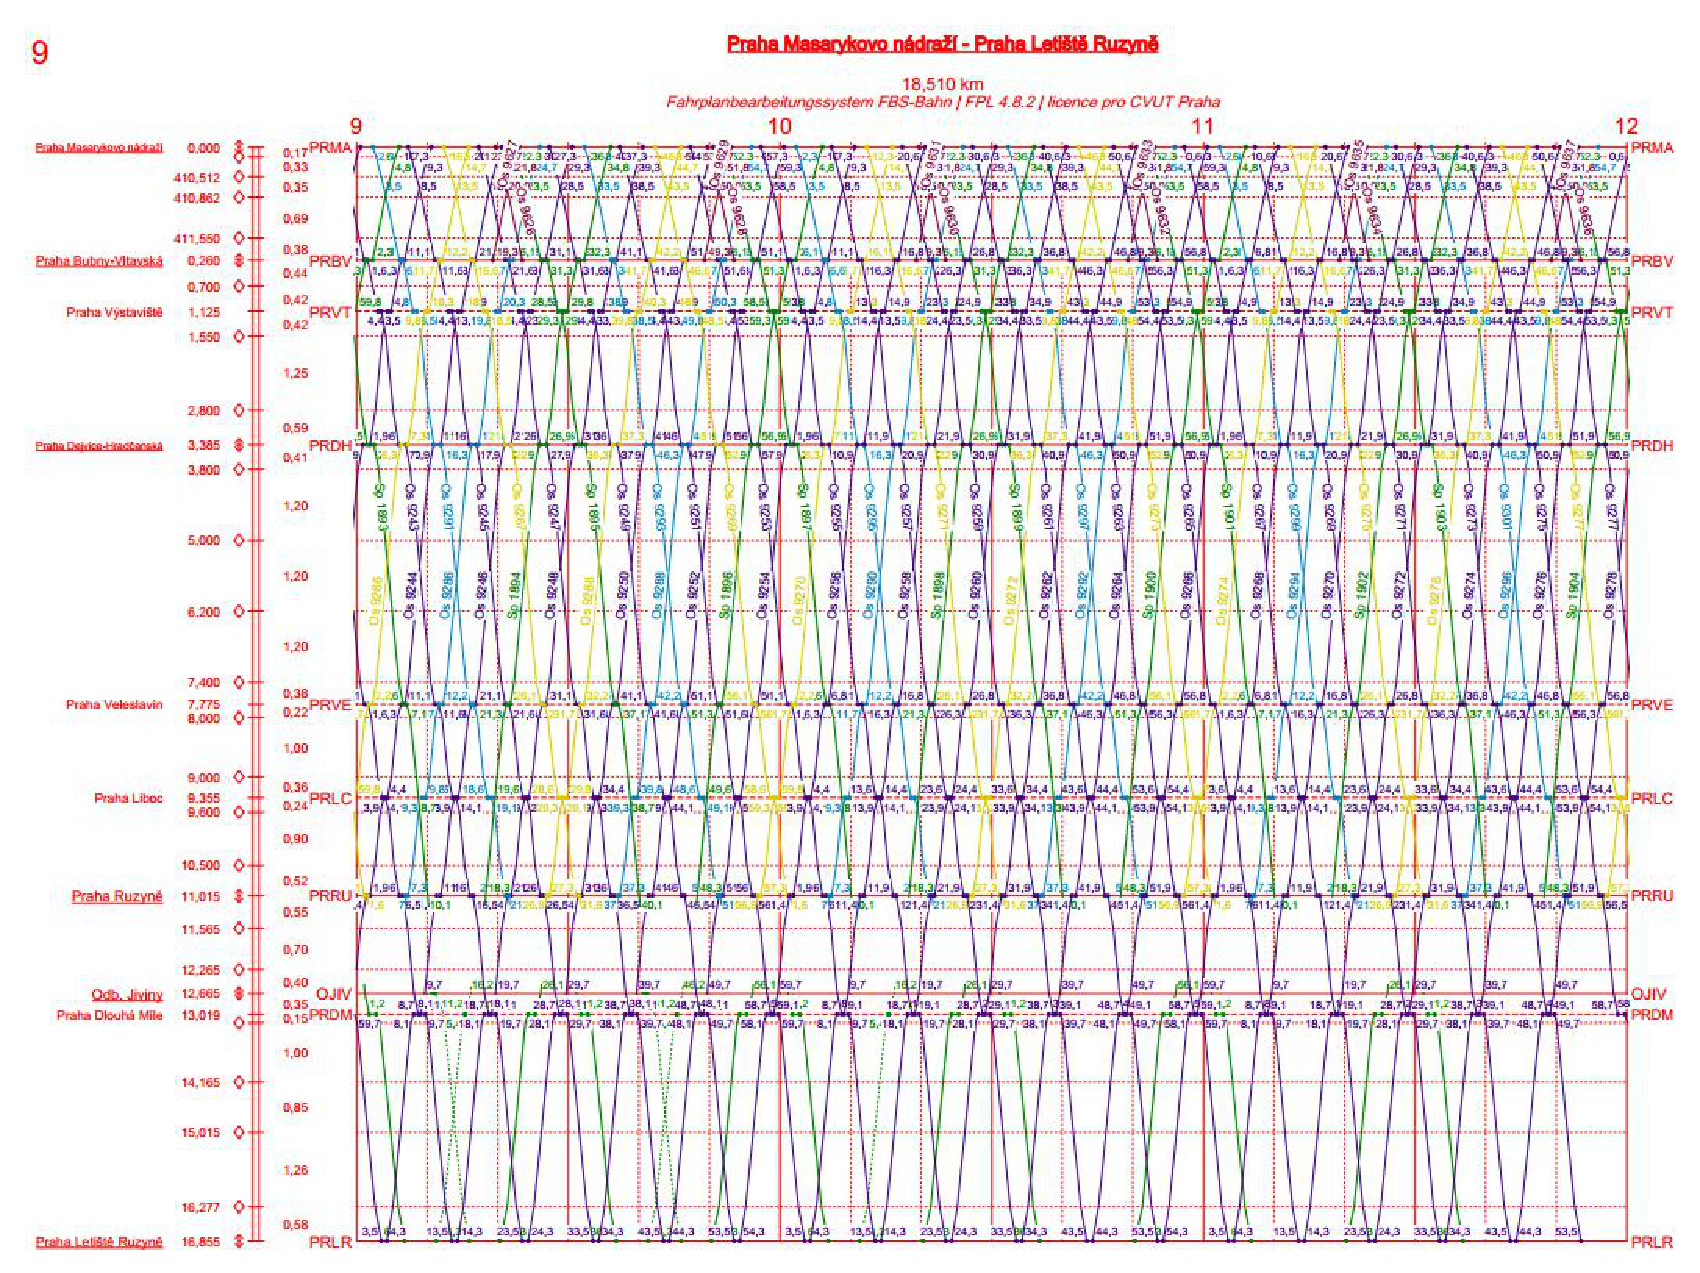
\includegraphics[width=\textwidth]{../img/kap1_studie_njr}
	\caption{Nákresný jízdní řád generovaný nástrojem FBS-Bahn pro diplomovou práci Koncepce obsluhy letiště Ruzyně kolejovou dopravou, M. Drábek~\cite{dipl_drabek}}
	\label{fig:studie_njr}
\end{figure}

\subsubsection{Aplikace v~modelové železnici}
Modelová železnice je co nejvěrnějším ztvárněním skutečné železnice ve zmenšeném měřítku. Za účelem napodobení skutečného provozu se nabízí jízdu vlaků na modelovém kolejišti organizovat podle grafikonu vlakové dopravy. Pokud se řízení vlaků na modelovém kolejišti věnuje více modelářů, v~rámci přípravy jsou jízdy vlaků rozplánovány a~zakresleny do nákresného jízdního řádu, který může být načrtnutý na papír.

Modeláři, kteří umí programovat, můžou vytvářet různé aplikace k~organizaci provozu na modelové železnici. Jednou z~nich je aplikace Grafikon \cite{Grafikon}, zobrazená na obrázku \ref{fig:grafikon_modely}. Aplikace umožňuje sestavit grafikon vlakové dopravy pro modelová kolejiště. Nákresný jízdní řád, který vykresluje, ale slouží pouze k~plánování a~není možné ho při řízení provozu na modelovém kolejišti měnit, třeba pro porovnání současného provozu s~původním plánem. Pro modeláře existují řešení, která umožňují řídit provoz na modelové železnici za pomoci počítače. Výrobci nástrojů pro řízení modelové železnice nabízí rozhraní, vůči kterým je možné vytvářet software sloužící k~sestavení vlakové cesty, kdy modelář může z~počítače měnit třeba nastavení výhybek. Takový software ale zcela nezachycuje proces organizace vlakové dopravy odpovídající skutečné situaci. Vytvářenou grafickou komponentu zobrazující nákresný jízdní řád by pak bylo možné zahrnout do nových nebo stávajících softwarových řešení, kterým by tato komponenta umožnila graficky zaznamenávat jízdy vlaků a~porovnávat je se sestaveným plánem.

\begin{figure}[ht]
	\centering
	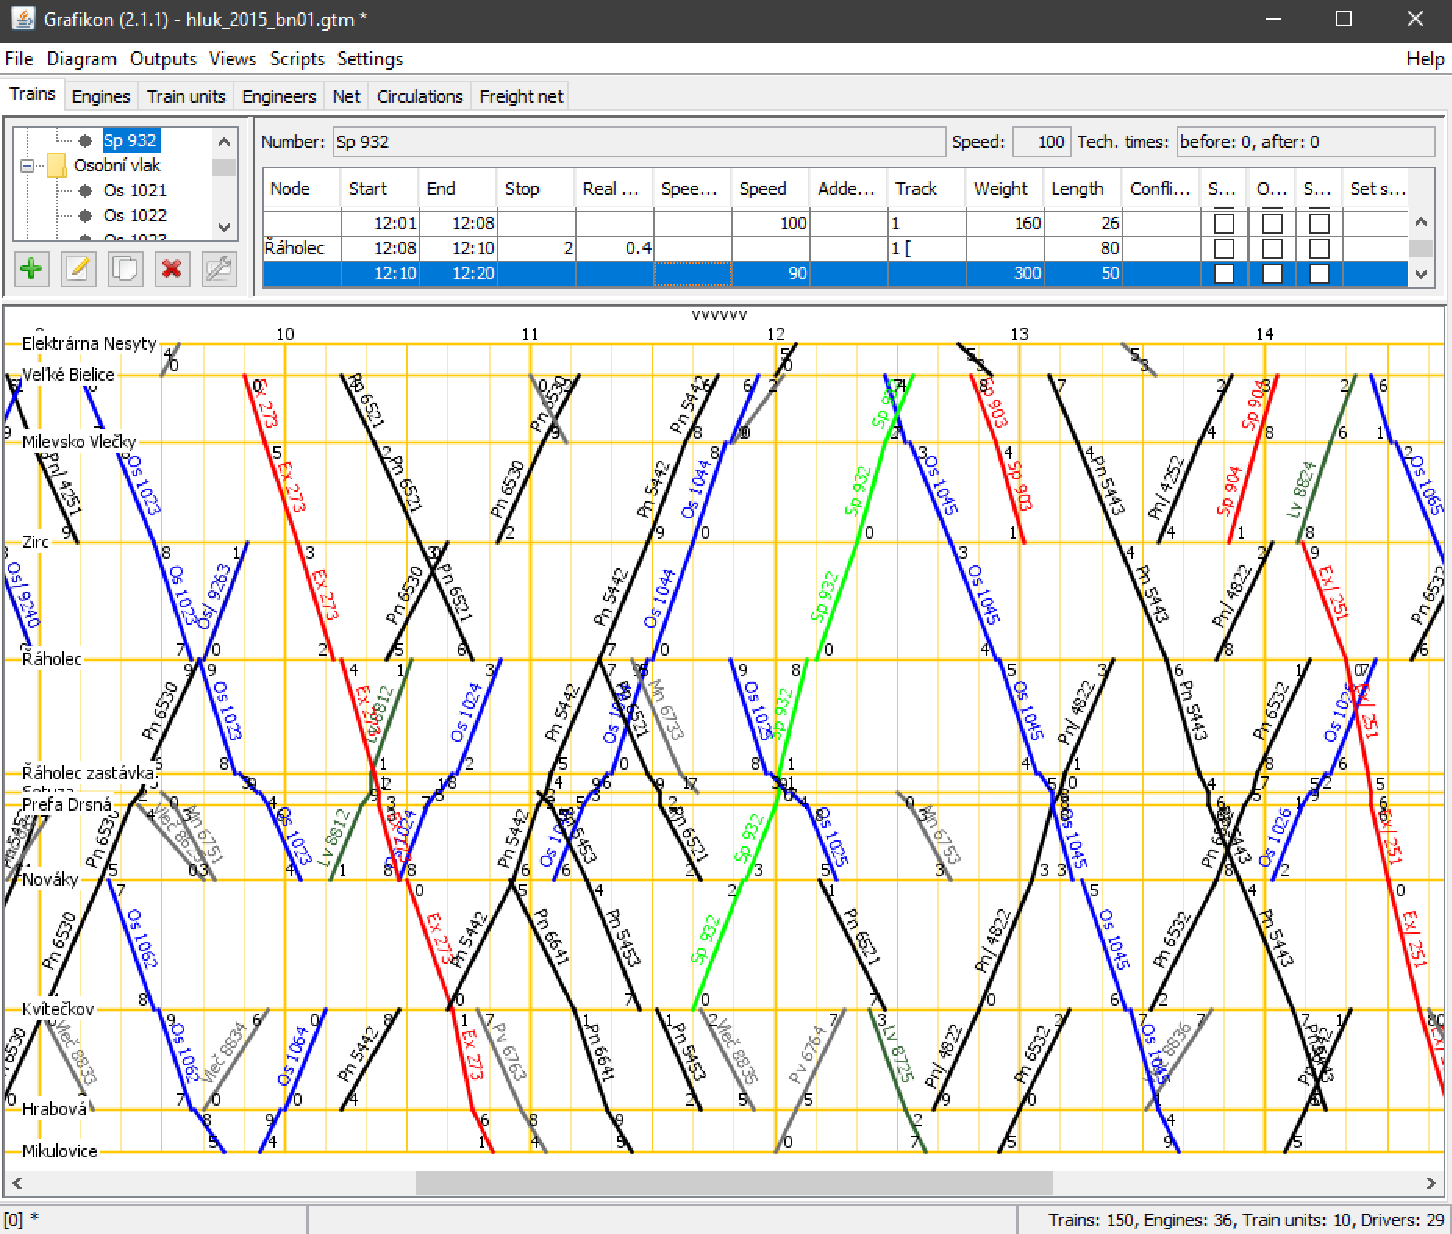
\includegraphics[width=\textwidth]{../img/kap1_grafikon_modely}
	\caption{Hlavní okno aplikace Grafikon určené pro modelové železnice}
	\label{fig:grafikon_modely}
\end{figure}

\subsubsection{Aplikace ve vlakových simulátorech}
\label{uvod:prace_s_grafikony_vlakove_dopravy:simulatory}
Námi vytvářený nástroj může být integrován do počítačových simulátorů, které se věnují řízení vlaku z~pozice strojvůdce. Na začátku tisíciletí vzniklo mnoho takových simulátorů a~her (Trainz \cite{Trainz}, MSTS \cite{MSTS}) vydávaných firmami, bez možnosti přístupu k~jejich zdrojovým kódům. V~posledních letech vznikly open-source projekty snažící se na základě těchto her vytvořit lepší simulátory s~větší konfigurovatelností, jelikož většina původních her už není dále vyvíjena a~podporována. Mezi tyto open-source simulátory patří OpenRails \cite{OpenRails} a~OpenBVE \cite{OpenBVE}. Oba dva tyto simulátory jsou napsané v~jazyce C\#, existují několik let a~jsou stále udržovány.

Simulátory, snažící se napodobit skutečný provoz na trati předpřipraveným scénářem jízd vlaků v~časovém intervalu několika hodin, by bylo užitečné doplnit pomůckami grafikonu vlakové dopravy. Hráči by byla dostupná (třeba v~okně vedle okna simulátoru) aplikace s~grafikonem vlakové dopravy, což v~současnosti ani jeden ze zmíněných open-source projektů nenabízí. Zajímavá by pak byla možnost hrát hru po síti s~dalšími lidmi (což už tyto simulátory umožňují) a~sledovat průběh hraného scénáře v~nákresném jízdním řádu v~porovnání s~původním plánem.

\section[Vývoj aplikací pro práci s~grafikonem vlakové dopravy]{Vývoj aplikací pro práci\\ s~grafikonem vlakové dopravy}

Zaměřme se na proces vývoje aplikací, které budou pracovat s~grafikonem vlakové dopravy. Všimněme si, že pro všechny uvedené příklady aplikací z~podkapitoly \ref{aplikace_gvd} je nezbytné zobrazovat nákresný jízdní řád. Bez komponenty aplikace, která je zodpovědná za jeho vykreslení, by se data z~grafikonu vlakové dopravy stala těžko spojitelnými množinami informací. Kdybychom se rozhodli vytvořit aplikaci pro práci s~grafikonem vlakové dopravy, stáli bychom tak vždy před rozhodnutím, jak tuto komponentu navrhnout. Pokud by existovala knihovna, která poskytne nástroje pro zobrazování nákresného jízdního řádu a~práci s~jeho obsahem, vývoj aplikací pracujících s~grafikonem vlakové dopravy by se tak ulehčil. Proto hlavní část této práce bude věnována vytváření takové knihovny. Námi vytvářenou knihovnu jsme se rozhodli pojmenovat GTTG (Generic Train Traffic Graph\footnote{Název knihovny jsme chtěli co nejvíce přiblížit anglickému názvu pro nákresný jízdní řád, který se lidmi orientující se ve vlakové dopravě většinou označuje jako train graph. Pro případ, že se s~názvem knihovny setká člověk bez představy o~tom, co nákresný jízdní řád je, jsme chtěli vystihnout to, že se nejedná o~graf zobrazující třeba železniční dvojkolí, ale graf zaznamenávající provoz na trati. Proto jsme přidali do názvu slovo traffic. Slovo generic na začátku názvu vystihuje záměr knihovny podporovat práci s~co největším množstvím nákresných jízdních řádů.}).

\subsection*{Knihovna pro platformu .NET}
Knihovnu, která bude představovat grafickou komponentu umožnující práci s~nákresným jízdním řádem, jsme se rozhodli naimplementovat v~jazyce C\#, který je součástí platformy .NET. Odůvodníme si, proč toto rozhodnutí není závadné a~seznámíme se s~knihovnou SkiaSharp \cite{SkiaSharp}, kterou budeme v~naší knihovně používat ke kreslení v~grafické komponentě.

\subsubsection*{Jazyk C\# a~.NET Standard}
Jelikož vytvářená knihovna bude reálně využívána hlavně modeláři, vývojáři nástrojů pro modelové železnice nebo programátory počítačových simulátorů, musí být snadno udržovatelná a~použitelná k~vytváření jejich vlastních implementací nákresného jízdního řádu. Protože knihovna bude většinou součástí nějaké aplikace s~uživatelským rozhraním, je vhodné, aby uživatelům knihovny bylo dostupné množství GUI frameworků, do kterých bude možné knihovnu jako grafickou komponentu zahrnout.

Protože jazyk C\# je jeden z~nejpoužívanějších objektově orientovaných jazyků a~nabízí mnoho GUI frameworků pro tvorbu desktopových aplikací, jeho výběr není v~rozporu s~tímto požadavkem a~můžeme ho použít. Silnou motivací, proč knihovnu implementovat právě v~tomto jazyce, je fakt, že oba dva zmíněné open-source simulátory jsou v~jazyce C\# napsané a~knihovnu tak bude možné v~těchto stávajících projektech využít.

Naší knihovnu bychom zároveň chtěli vytvořit tak, aby byla v~rámci platformy .NET co nejvíce použitelná. Každý spustitelný program, který v~jazyce C\# napíšeme, může být spuštěn pouze vůči některému z~běhových prostředí. Původním běhovým prostředím platformy .NET je .NET Framework, který je určen pro operační systém Windows. Vedle tohoto běhového prostředí existuje Mono, které bylo vytvořeno jako open-source náhražka .NET Frameworku pro operační systémy Linux a~MacOS. V~posledních letech vzniklo běhové prostředí .NET Core, jehož vývoj je řízen společností Microsoft a~je možné ho použít na operačních systémech Windows, Linux a~MacOS. Je v~plánu nahradit .NET Framework a~Mono právě tímto novým běhovým prostředím. Aby bylo možné vytvářet knihovny, které budou použitelné všemi běhovými prostředími, vzniklo rozhraní .NET Standard. Knihovny, které vůči .NET Standard implementujeme, můžou stále používat skoro stejnou část používaných tříd a~implementací, které jsou nabízeny například v~rámci běhového prostředí .NET Framework. Aby .NET Standard docílilo přenositelnosti mezi více běhovými prostředími, určuje rozhraní, které běhová prostředí musí implementovat, aby kód knihovny .NET Standard mohl být na konkrétním běhovém prostředí vykonáván.
Jelikož vytvářená grafická komponenta bude často umístěna v~aplikaci s~GUI frameworkem, který je spustitelný vůči jednomu běhovému prostředí, bude naše knihovna přenositelná v~rámci rozhraní .NET Standard.

\subsubsection*{SkiaSharp}
Naše knihovna potřebuje nějaký nástroj, který bude sloužit k~vykreslování nákresného jízdního řádu. Práce s~tímto nástrojem by měla být lehká, jelikož ho budeme chtít nabídnout uživatelům naší knihovny pro implementaci jejich vlastních typů nákresných jízdních řádů.

Pro jazyk C\# existuje knihovna SkiaSharp, jako wrapper\footnote{Označení pro knihovnu pracující s~cizí funkcionalitou, kterou vhodně upravuje nebo zpřístupňuje uživateli wrapperu, většinou s~žádnými změnami v~sémantice cizí funkcionality, které chce uživatel wrapperu využívat. SkiaSharp jako wrapper překládá volání funkcí z~jazyka C\# do kódu knihovny Skia implementované v~jazyce C++.} nad vysoce výkonnou 2D grafickou knihovnou Skia napsanou v~jazyce C++. Skia nabízí pro uživatele lehké kreslení různých komplexních typů čar a~textu, které nákresné jízdní řády obsahují. Práce s~knihovnou SkiaSharp je lehká, díky její dostupné dokumentaci, zcela nutné pro případ, kdy ji chceme také nabídnout uživatelům naší knihovny.

Knihovna SkiaSharp je navíc přenositelná v~rámci rozhraní .NET Standard, čili je naší knihovnou použitelná a~splňuje i~všechny naše požadavky na grafický nástroj, který bude naše knihovna používat pro vykreslování nákresného jízdního řádu.

\subsection*{Implementace vlastní aplikace}
Abychom mohli předvést využití naší knihovny, rozhodli jsme se vytvořit vzorovou aplikaci pro práci s~grafikonem vlakové dopravy. Aplikace uživatelům umožní prohlížet nákresné jízdní řády vydávané Správou železniční dopravní cesty. Ověříme tak schopnost knihovny podporovat zobrazení specifické implementace nákresného jízdního řádu. Abychom předvedli, jak knihovna podporuje editaci nákresného jízdního řádu, přidáme mód vytvářející náhodnou dopravní situaci na trati, v~rámci které bude možné upravovat interaktivně v~nákresném jízdním řádu jízdy jednotlivých vlaků.

\section{Cíle práce}
\label{kap1:cile_prace}
\begin{enumerate}[label=\color{goalcolor}\textbf{G{\arabic*}}]
	\item \label{uvod:cil:knihovna}Vytvořit knihovnu pro platformu .NET, představující grafickou komponentu, umožňující práci s~nákresnými jízdními řády
	\begin{enumerate}[label=\color{goalcolor}\textbf{\alph*})]
		\item \label{uvod:cil:knihovna:ruzne_typy_njr} Podporovat zobrazování různých typů nákresných jízdních řádů
		\item \label{uvod:cil:knihovna:integrace_do_aplikaci} Podporovat integraci komponenty do aplikací pracujících s~grafikonem vlakové dopravy
		\item \label{uvod:cil:knihovna:replikace_chovani} Umožnit replikovat chování existujících aplikací pracujících s~grafikonem vlakové dopravy
		\item \label{uvod:cil:knihovna:dotnet_standard} Zajistit přenositelnost knihovny na úrovni .NET Standard
	\end{enumerate}

	\item \label{uvod:cil:aplikace} Použít tuto knihovnu pro implementaci aplikace, která bude sloužit pro práci s~grafikonem vlakové dopravy
	\begin{enumerate}[label=\color{goalcolor}\textbf{\alph*})]
		\item \label{uvod:cil:aplikace:staticke_zobrazeni} Aplikace bude interaktivně zobrazovat listy nákresného jízdního řádu vydávané Správou železniční dopravní cesty.
		\item \label{uvod:cil:aplikace:dynamicke_zobrazeni} Aplikace bude pro ilustrační účely knihovny nabízet mód simulující provoz na trati, v~jehož rámci bude možné upravovat výhledovou dopravu.
		\item \label{uvod:cil:aplikace:vice_gui} Aplikace bude navržena tak, aby část pracující s~modelem dat, představující logiku aplikace, byla zapojitelná do více GUI frameworků platformy .NET.
	\end{enumerate}
	
	\item \label{uvod:cil:skia} Ověřit možnost využití 2D grafické knihovny SkiaSharp pro zobrazování komplexních dat obsažených v~nákresných jízdních řádech
\end{enumerate}

\chapter{Analýza požadavků pro práci s~knihovnou GTTG}
\label{kap:spec}
Z~kapitoly \ref{kap:uvod} jsme získali základní představu o~tom, jaký účel bude knihovna GTTG splňovat a~určili jsme si cíle, kterými se při implementaci knihovny budeme řídit. V~této kapitole si tyto cíle více upřesníme a~vytvoříme detailní souhrn požadavků, představujících kritéria pro správný výběr implementace. Požadavky je možné rozdělit do dvou hlavních kategorií:

\begin{itemize}
	\item Požadavky na chování grafické komponenty jako okna, v~kterém je zobrazován nákresný jízdní řád 
	\item Požadavky na vykreslování nákresného jízdního řádu a~práci s~jeho obsahem
\end{itemize}

\section{Požadavky na chování grafické komponenty}
\label{kap:spec:komponenta}
V~této části vytvoříme požadavky určující chování grafické komponenty, která představuje okno s vykreslovaným obsahem. Určíme, jak se komponenta chová, například v~rámci integrace s~uživatelským rozhraním. Určením požadavků pro práci s~touto komponentou vytvoříme prostředí, které umožní práci s~nákresným jízdním řádem. Při určování těchto požadavků jsme zejména brali ohled na náš cíl zajistit replikovatelnost chování původních aplikací. Narozdíl od původních aplikací by ale knihovna měla nabízet i~nové chování, které by zlepšilo interakci uživatelů s~komponentou.

\subsubsection*{Interakce uživatelů s~komponentou}
Jelikož vytváříme knihovnu pro více aplikací, měli bychom podporovat co největší množinu operací, kterými lze komponentu modifikovat. Aplikace pracující s~knihovnou si z~této množiny operací vybere pouze ty, které chce podporovat. V~této části určíme požadavky, které umožní interakcemi uživatele s~komponentou měnit zobrazovaný obsah komponenty. Podívejme se, jak existující aplikace zmíněné v~podkapitole \ref{aplikace_gvd} umožňují uživatelům pracovat s~komponentou. Na obrázku \ref{fig:spec:oltis_grafikon} se nachází aplikace od OLTIS Group. Na pravé hraně komponenty nabízí posuvník pro změnu zobrazované části traťového úseku. Stejným způsobem komponenta umožňuje na horizontále výběr zobrazovaného časového intervalu. Uživateli je tak zobrazen jen nějaký výřez z~celého obsahu nákresného jízdního řádu, který vytváří hranice, v~rámci kterých je možné zobrazení měnit posuvníky. Grafické znázornění hranic a~zobrazované části nákresného jízdního řádu v~komponentě se nachází na obrázku \ref{fig:spec:border}. Jelikož se stejným způsobem chovají i~ostatní existující aplikace a~toto chování chceme zachovat i~u~nových aplikací pracujících s~knihovnou, definujeme následující požadavky.

\begin{enumerate}[label=\color{reqcolor}\textbf{R{\arabic*}}]
	\item \label{spec:req:interaction_trans1} Komponentou zobrazovaný obsah se nachází v~ohraničení, které je určeno zobrazitelným obsahem nákresného jízdního řádu
	\item \label{spec:req:interaction_trans2} Komponentou zobrazovaný obsah je možné měnit posunem po vertikální a~horizontální ose v~rámci ohraničení definovaném \ref{spec:req:interaction_trans1}
\end{enumerate}

\begin{figure}[!htb]
	\centering
	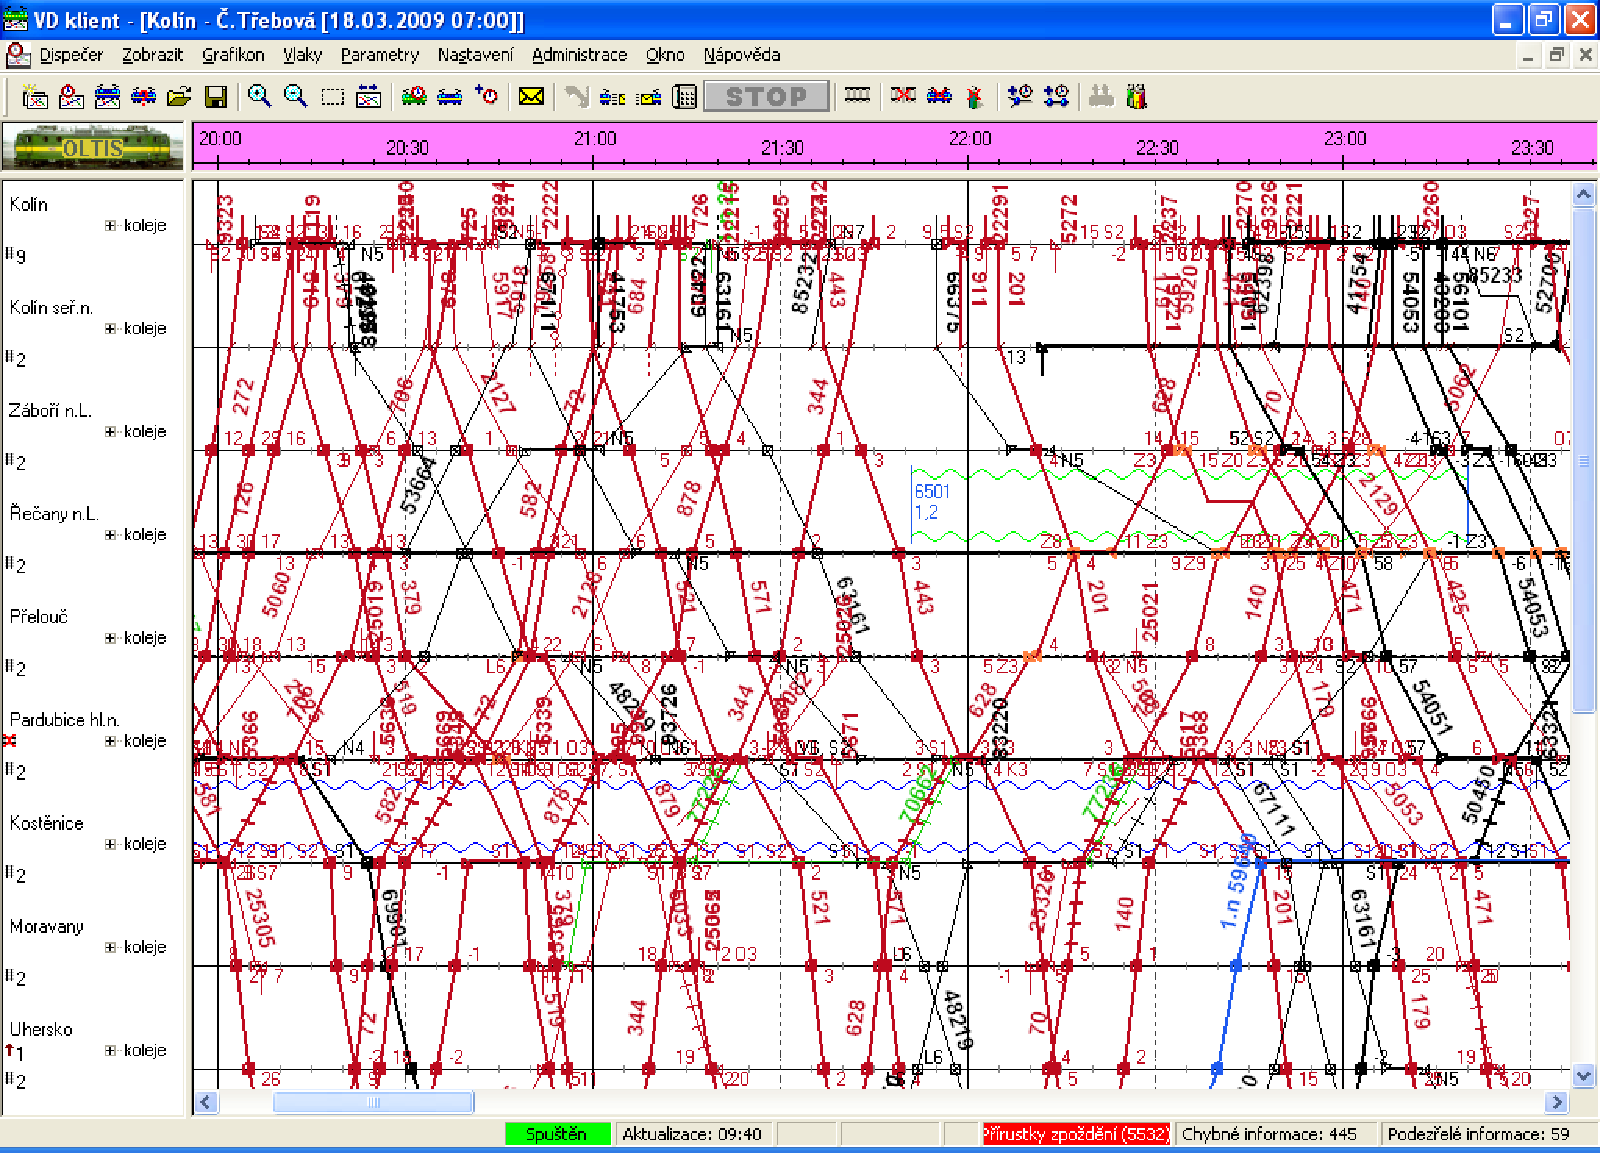
\includegraphics[width=0.9\textwidth]{../img/kap1_ISOR_window}
	\caption{Aplikace od OLTIS Group s~posuvníky, převzato ze stránky společnosti~\cite{ISOR_CDS}}
	\label{fig:spec:oltis_grafikon}
\end{figure}

\begin{figure}[!htb]
	\centering
	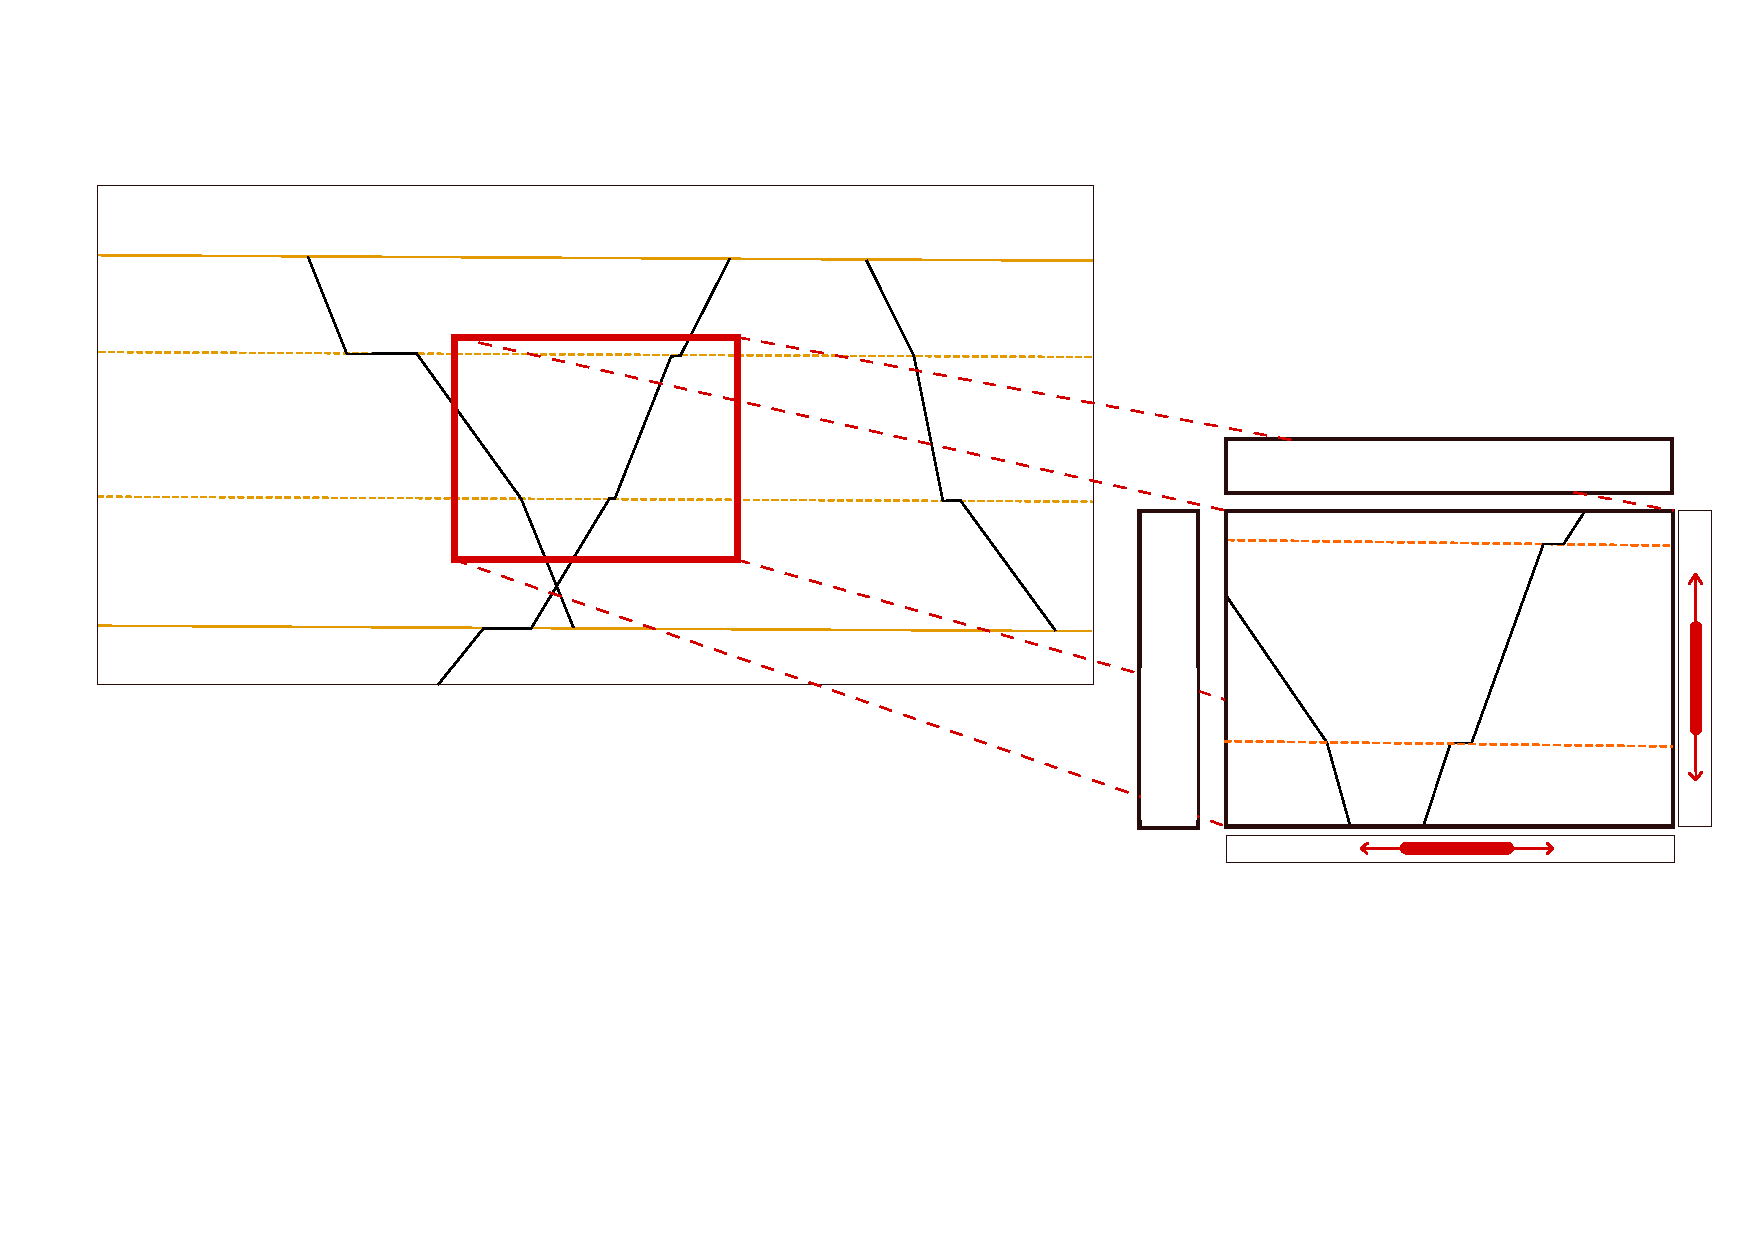
\includegraphics[width=0.9\textwidth]{../img/kap2_ohraniceni_definice}
	\caption{Komponentou zobrazovaný obsah a~ohraničení určené zobrazitelným obsahem nákresného jízdního řádu}
	\label{fig:spec:border}
\end{figure}

\pagebreak
Existující aplikace umožňují měnit zobrazený obsah pouze posunem. Interakci uživatelů s~grafickou komponentou bychom chtěli zlepšit přidáním možnosti zobrazovaný obsah přiblížit a~oddálit, jak je ukázáno na obrázku \ref{fig:spec:zoom}. Pohled se bude oddalovat nebo přibližovat vůči zobrazovanému bodu, jehož umístění na plátně bude stále stejné -- v~případě, že uživatel bude zobrazení přibližovat myší, bude tento bod odpovídat kurzoru myši. V~případě, že operace oddálení způsobí, že by se komponenta nacházela mimo ohraničení zabrazitelného obsahu a~porušila by požadavek \ref{spec:req:interaction_trans1}, je potřeba vzniklou situaci deterministicky opravit. Případ, kdy k~takové situaci dochází, je uveden na obrázku \ref{fig:spec:zoom_out_of_bounds}.
\pagebreak
\begin{enumerate}[label=\color{reqcolor}\textbf{R{\arabic*}},resume]
	\item \label{spec:req:interaction_zoom1} Komponenta podporuje operace přiblížení a~oddálení pohledu. Při těchto operacích je určen v~zobrazení bod, který po operaci v~komponentě nezmění svou polohu
	\item \label{spec:req:interaction_zoom2} V~případě, že by se oddálení komponenty dostalo mimo ohraničení definované v~\ref{spec:req:interaction_trans1}, použije knihovna deterministický postup, který operaci oddálení vhodně opraví
\end{enumerate}

\begin{figure}[!htb]
	\centering
	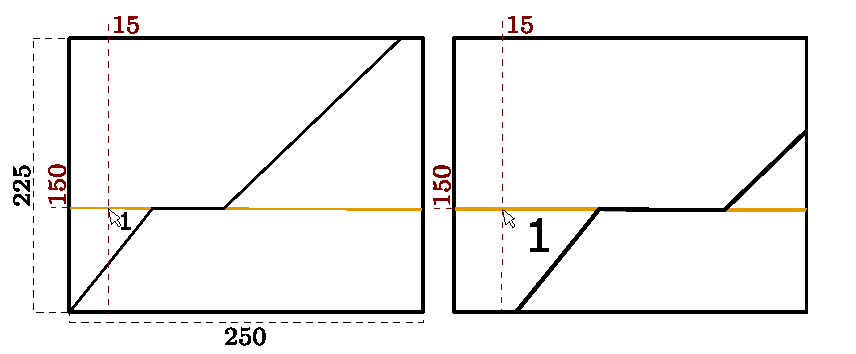
\includegraphics[width=0.9\textwidth]{../img/kap2_scale_example}
	\caption{Přiblížení pohledu na bod v~komponentě, kde se nachází kurzor myši. Tento bod zůstává po přiblížení v~komponentě na stejném místě.}
	\label{fig:spec:zoom}
\end{figure}

\begin{figure}[!htb]
	\centering
	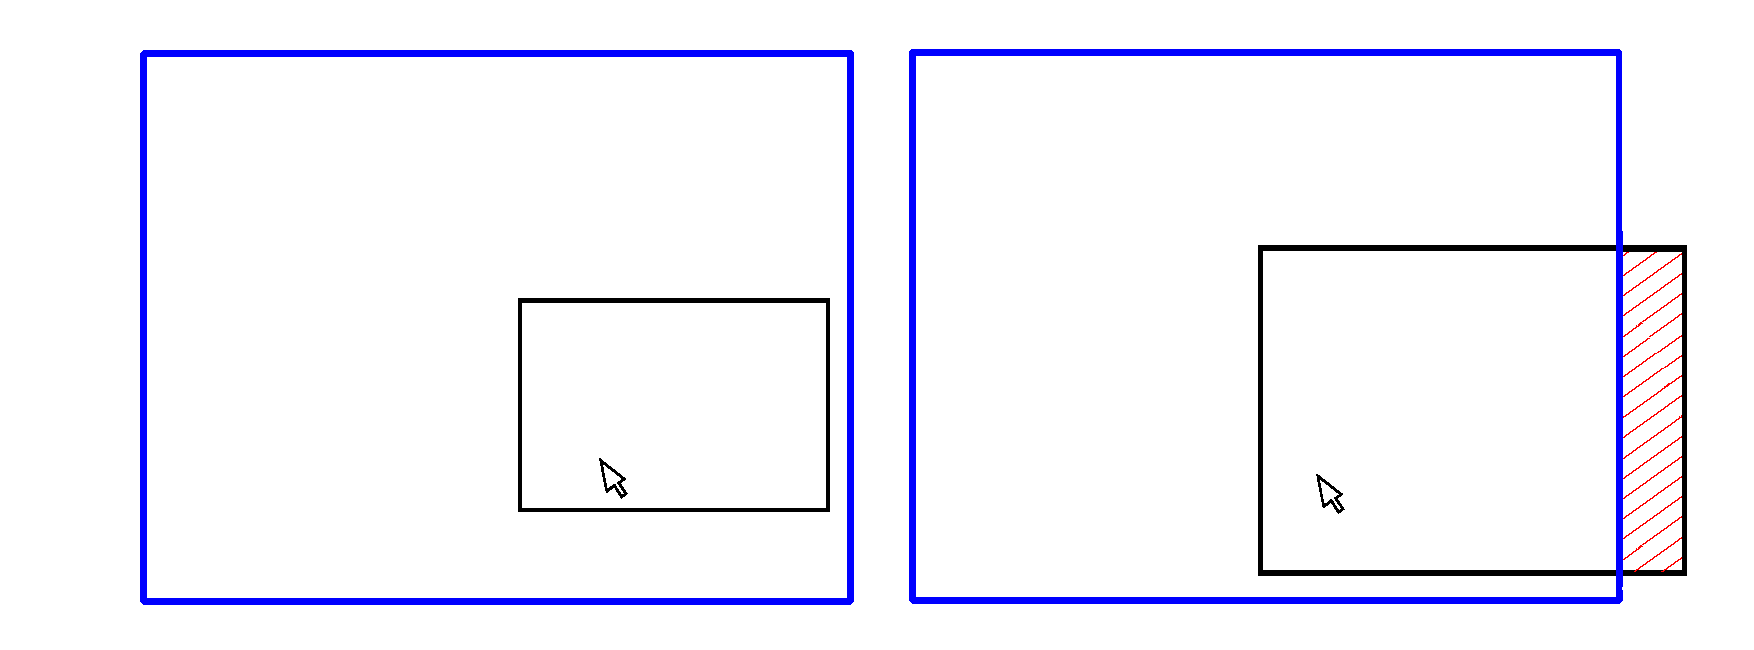
\includegraphics[width=0.9\textwidth]{../img/kap2_scale_example_out_of_bounds}
	\caption{Situace, kdy se komponenta po oddálení nachází mimo ohraničení definované \ref{spec:req:interaction_trans1}.}
	\label{fig:spec:zoom_out_of_bounds}
\end{figure}

\subsubsection*{Mapování časových intervalů na horizontální osu}
\label{kap2:time_intervals}
Víme, že horizontální osa grafu, v~němž je nákresný jízdní řád umístěn, značí čas. V~nákresném jízdním řádu pak zobrazujeme provoz z~nějakého časového intervalu určeného právě časy na horizontální ose. Pokud zobrazujeme výřez z~nákresného jízdního řádu, časový interval tohoto výřezu je podinterval zmíněného časového intervalu. Znázornění těchto intervalů se nachází na obrázku \ref{fig:spec:casove_intervaly}. Jelikož se zmíněnými intervaly budeme často pracovat, zavedeme jejich označení:

\begin{enumerate}[label=\color{reqcolor}\textbf{R{\arabic*}},resume]
	\item \label{spec:req:int1} Komponenta mapuje časový interval, který se nazývá \textit{časový interval zobrazení}, na body horizontální osy komponenty
	\item \label{spec:req:int2}	Komponenta mapuje časový interval, který se nazývá \textit{časový interval ohraničení}, na body horizontální osy v~rámci ohraničení definovaného \ref{spec:req:interaction_trans1}
\end{enumerate}

\begin{figure}[!htb]
	\centering
	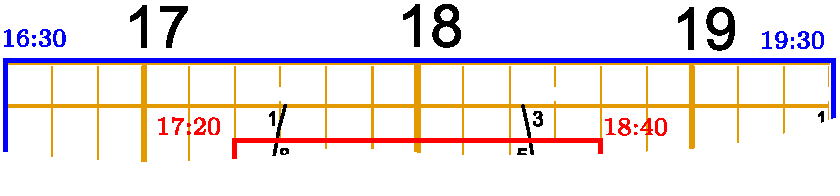
\includegraphics[width=\textwidth]{../img/kap2_time_intervals}
	\caption{Časový interval zobrazení (červeně) a~ohraničení (modře).}
	\label{fig:spec:casove_intervaly}
\end{figure}

\subsubsection*{Změna velikosti komponenty a~hranic obsahu}
Jelikož bude komponenta obvykle součástí uživatelského rozhraní, může být její velikost v~rámci procesu rozmístění uživatelského rozhraní změněna. Na obrázku \ref{fig:spec:zmena_velikosti_horizontalni} je zobrazena změna šířky komponenty. Pokud porovnáme původní a~nové zobrazení po změně, vidíme, že se časový interval zobrazení nezměnil. Existující aplikace se při změně šířky komponenty chovají stejným způsobem, bude to tedy chování komponenty, které od knihovny při změně šířky požadujeme.

\begin{enumerate}[label=\color{reqcolor}\textbf{R{\arabic*}},resume]
	\item \label{spec:req:width_mod1} Při změně velikosti komponenty zůstává časový interval zobrazení definovaný \ref{spec:req:int1} nezměněn
\end{enumerate}

\begin{figure}[!htb]
	\centering
	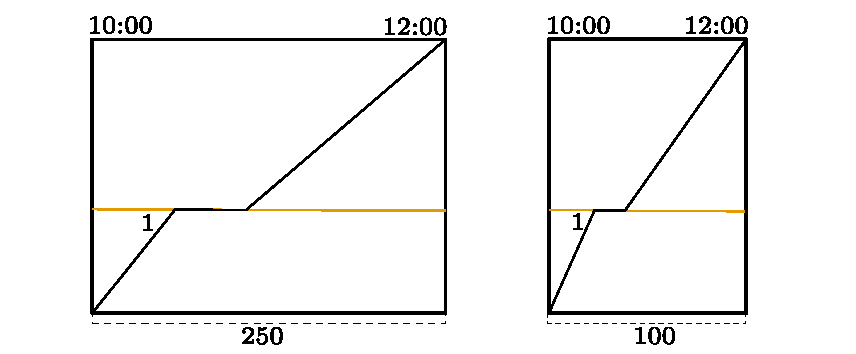
\includegraphics[width=\textwidth]{../img/kap2_horizontal_resize}
	\caption{Nezměněný časový interval při změně šířky komponenty}
	\label{fig:spec:zmena_velikosti_horizontalni}
\end{figure}

Při změně výšky komponenty existuje více způsobů, jak zobrazení upravit. Jednou z~možností je použít stejné chování, které se používá při změně šířky komponenty. Zobrazovaný obsah by tak zůstal stejný -- v~nejjednodušším scénaři budou dopravní body v~komponentě rozmístěny podle poměru jejich kilometrické vzdálenosti. Chování je znázorněno na obrázku \ref{fig:spec:zmena_velikosti_vertikalni_modifikace_1}.

\begin{enumerate}[label=\color{reqcolor}\textbf{R{\arabic*}},resume]
	\item \label{spec:req:height_mod1}	Při změně výšky komponenty může zůstat zobrazovaný obsah komponenty nezměněn a~jeho rozmístění je vzhledem k~nové výšce proporčně upraveno
\end{enumerate}

\begin{figure}[!htb]
	\centering
	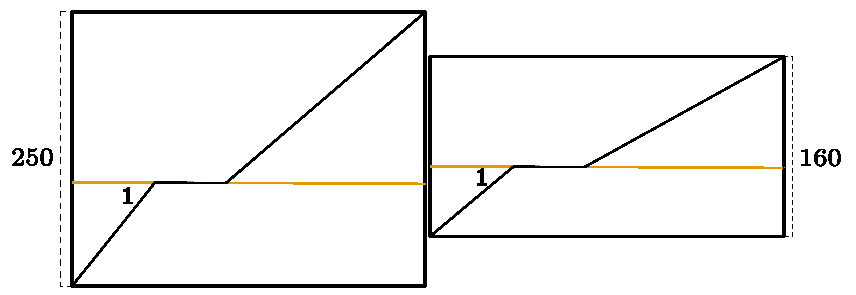
\includegraphics[width=\textwidth]{../img/kap2_vertical_resize_proportional}
	\caption{Proporční rozmístění stejného obsahu při změně výšky komponenty}
	\label{fig:spec:zmena_velikosti_vertikalni_modifikace_1}
\end{figure}

Problémem předchozího požadavku je chování v~případě, kdy je výška komponenty příliš malá. Zobrazované informace v~komponentě jsou pak nepřehledné. Proto chceme vedle tohoto řešení nabídnout jiné, které zachová původní rozmístění. V~případě zmenšení výšky se ze zobrazovaného obsahu zobrazí jeho výřez a~nově skrytou část původního obsahu je možné zobrazit posunutím. Při zvětšení výšky se k~původnímu obsahu přidá doposud skrytá zobrazitelná část navazující na původní obsah. Zvětšení výšky je možné tímto způsobem aplikovat, pokud je komponenta stále umístěna v~hranicích zobrazitelného obsahu. Chování je znázorněno na obrázku \ref{fig:spec:zmena_velikosti_vertikalni_modifikace_2}.

\begin{enumerate}[label=\color{reqcolor}\textbf{R{\arabic*}},resume]
	\item \label{spec:req:height_mod2} Je možné zmenšit výšku komponenty tak, aby byla zobrazena jen část původního výřezu
	\item \label{spec:req:height_mod3} Je možné zvětšit výšku komponenty tak, aby byla zobrazena původní část s~nově odkrytou částí obsahu. Modifikace je možná, pokud zvětšení komponenty nepřekročí ohraničení definované \ref{spec:req:interaction_trans1}
\end{enumerate}

\begin{figure}[!htb]
	\centering					
	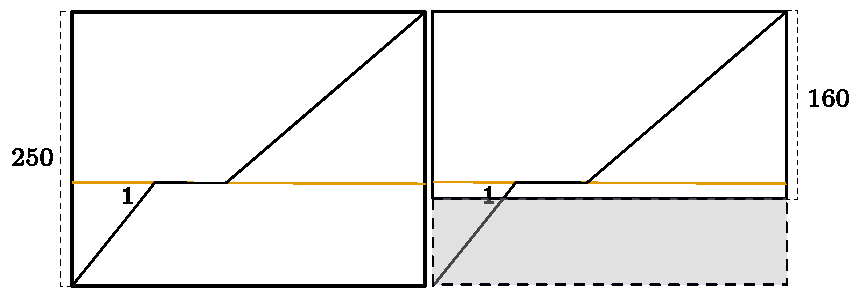
\includegraphics[width=\textwidth]{../img/kap2_vertical_resize_view_change}
	\caption{Změna zobrazeného obsahu při změně výšky komponenty}
	\label{fig:spec:zmena_velikosti_vertikalni_modifikace_2}
\end{figure}

\subsubsection*{Modifikace časových intervalů}
\label{kap2:modifikace_cas_intervaly}
V~této části popíšeme už zavedené modifikace ve formě nastavování časových intervalů. Je užitečné, aby zobrazovaný obsah, odpovídající nějakému časovému intervalu, bylo možné podle určení tohoto intervalu nastavit. Uvedeme si příklad, kdy se tento způsob modifikace uplatňuje. Aplikace často nabízí možnost zobrazit obsah v~přednastavených úsecích několika hodin (například 2h, 4h, 6h). Pokud například komponenta zobrazuje interval o~délce dvě hodiny (14:00 - 16:00), je možné změnit obsah komponenty tak, aby nyní zobrazoval interval šesti hodin (12:00 - 18:00). Tato modifikace je zachycena na obrázku \ref{fig:spec:zmena_casoveho_intervalu_zobrazeni}. Pokud toto chování zobecníme, požadujeme, aby mohl být nastaven jakýkoliv podinterval časového intervalu ohraničení.

\begin{enumerate}[label=\color{reqcolor}\textbf{R{\arabic*}},resume]
	\item \label{spec:req:time_mod1} Zobrazení může být změněno tak, aby obsah komponenty odpovídal zobrazení nově nastavovaného časového intervalu zobrazení, který musí být součástí časového intervalu ohraničení
\end{enumerate}

\begin{figure}[!htb]
	\centering					
	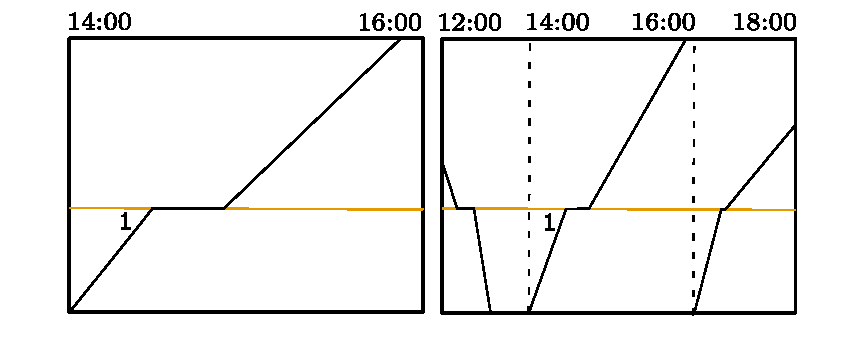
\includegraphics[width=\textwidth]{../img/kap2_time_interval_change}
	\caption{Změna časového intervalu zobrazení}
	\label{fig:spec:zmena_casoveho_intervalu_zobrazeni}
\end{figure}

Existují případy, kdy se v komponentě zobrazuje obsah odpovídající aktuálnímu času v~rámci nějakého časového intervalu (například okno 12:00 - 18:00 s~aktuálním časem 15:00). Periodicky se pak například po hodině celé toto časové okno o~hodinu posune. Chtěli bychom proto umožnit i~změnu časového intervalu ohraničení.

\begin{enumerate}[label=\color{reqcolor}\textbf{R{\arabic*}},resume]
	\item \label{spec:req:time_mod2} Zobrazitelný obsah je možné změnit nastavením nového časového intervalu ohraničení. V~rámci změny časového intervalu ohraničení je nutné poskytnout podinterval, který bude nastaven jako časový interval zobrazení
\end{enumerate}

Navíc se knihovna musí jednotně chovat ve změně vertikální polohy komponenty v~rámci ohraničení při změně časového intervalu. Jako nejvhodnější se ukazuje vertikální umístění komponenty neměnit, jelikož můžeme změnou časového intervalu vytvořit posun, zobrazující část původních informací z~výřezu na stejné vertikální úrovni.

\begin{enumerate}[label=\color{reqcolor}\textbf{R{\arabic*}},resume]
	\item \label{spec:req:time_mod3} Změny zobrazení určené časovými intervaly nemění vertikální umístění komponenty v~ohraničení definovaném \ref{spec:req:interaction_trans1}
\end{enumerate}

\subsubsection*{Podporované jednotky určující velikost komponenty}
Doposud jsme neurčili, v~jakých jednotkách se měří velikosti komponenty a~jejího ohraničení. Jelikož komponenta zobrazuje nějaké plátno, které je určeno jednotkami pixelů, požadujeme, aby s~jejími velikostmi bylo možné pracovat v~různých jednotkách pixelů -- například jednotkách pixelů nezávislých na zařízení a~jednotkách pixelů zařízení. Pokud by se vývojář rozhodl používat jednotky pixelů zařízení, knihovna by mu měla poskytnout možnost zjistit aktuální DPI\footnote{dots per inch} hodnotu zařízení, na kterém je aplikace spuštěna, aby mohl případně zajistit třeba stejnou velikost textu mezi různými zařízeními.

\begin{enumerate}[label=\color{reqcolor}\textbf{R{\arabic*}},resume]
	\item \label{spec:req:unit1} Velikost komponenty může být udávána v~různých jednotkách pixelů:
		\begin{itemize}
			\item	Jednotky pixelů nezávislých na zařízení
			\item	Jednotky pixelů zařízení
		\end{itemize} 
	\item \label{spec:req:unit2} V~případě práce s~jednotkami pixelů zařízení bude mít vývojář možnost zjistit hodnotu DPI zařízení  
\end{enumerate}

\subsubsection*{Stav pro určení zobrazovaného obsahu}
Předchozími požadavky jsme vytvořili základ pro prostředí, v~kterém je možné pracovat se zobrazením nákresného jízdního řádu. Toto prostředí je popsáno informacemi, které tvoří jeho stav.

\begin{enumerate}[label=\color{reqcolor}\textbf{R{\arabic*}},resume]
\item \label{spec:req:state} Aby bylo možné určit, jaký obsah se má v~komponentě zobrazit, zahrne komponenta do svého stavu:
	\begin{itemize}
		\item Velikosti komponenty a~ohraničení
		\item Umístění komponenty v~ohraničení definovaném \ref{spec:req:interaction_trans1}
		\item Faktor škálování, který určuje, jak moc je zobrazení v~komponentě přiblížené a~odpovídá násobkům neupravené velikosti
		\item Časový interval zobrazení a~časový interval ohraničení
	\end{itemize}
\end{enumerate}

\section{Vykreslení obsahu nákresných jízdních řádů}
\label{kap:spec:obsah_njr}
Tato část určuje požadavky, které souvisí s~vykreslováním obsahu komponenty, jejíž chování jsme určili požadavky předchozí části. Dále uvedeme požadavky, které vývojáři ulehčí přípravu nákresného jízdního řádu k~jeho vykreslení. Tyto požadavky nejsou tak přesné jako v~předchozí části, ale spíše určují směr, jakým se implementace knihovny musí vydat, aby mohla být dostatečně rozšiřitelná a~využitelná implementacemi více typů nákresných jízdních řádů.

\subsection*{Plátno pro kreslení}
Knihovna by měla vývojářům ulehčit práci při vykreslování nákresného jízdního řádu. Změnou stavu komponenty se neustále mění obsah, který by měl být zobrazen. Při každé změně je potřeba na komponentě zobrazit nově odpovídající část z~celého nákresného jízdního řádu. Pokud bychom po knihovně požadovali co nejméně, stačilo by, aby vývojáři byla dostupná informace o~stavu komponenty určena v~\ref{spec:req:state} a~plátno, jehož obsah je zobrazen v~komponentě. Vývojář by pak musel spočítat, jaký obsah se má zobrazit a~tento obsah vykreslit. Takový přístup je ale pro vývojáře knihovny velmi náročný. Knihovna by mu měla nabídnout plátno, na které by se zobrazil celý obsah nákresného jízdního řádu a~knihovna by pak sama přepočítala, jaký výřez z~plátna se má v~komponentě zobrazit.

Knihovna by ale měla nabízet i~možnost pracovat pouze s~částí plátna, která je zobrazena v~komponentě. Tato změna je užitečná v~případě, pokud chceme v~komponentě zobrazit informace, které nejsou součástí nákresného jízdního řádu, ale mají informativní charakter v~rámci aplikace, jako je současné datum nebo notifikace o~změně související s~nákresným jízdním řádem. Během kreslení tak může uživatel pohled na plátno měnit.

\begin{enumerate}[label=\color{reqcolor}\textbf{R{\arabic*}},resume]
	\item \label{spec:req:canvas1} Uživateli je přístupné plátno, které odpovídá obsahu ohraničení definovaném \ref{spec:req:interaction_trans1}
	\item \label{spec:req:canvas2} Uživateli je přístupný pohled na plátno definované v~\ref{spec:req:canvas1}. Obsah tohoto pohledu je vždy vykreslen v~komponentě
\end{enumerate}

\subsubsection*{Převod časových údajů na horizontální osu}
Jelikož vývojář pracuje s~nákresným jízdním řádem, kde horizontální osa představuje časový interval, chceme, aby knihovna nabízela nástroje umožňující převod mezi horizontální polohou bodu na plátně a~časovými údaji. Pokud vývojář bude kreslit průběh jízdy vlaku, nejspíše využije tento nástroj pro přepočítání časového údaje příjezdu, odjezdu nebo průjezdu do horizontální polohy na plátně, z~které povede čáru značící část průběhu jízdy vlaku.

\begin{enumerate}[label=\color{reqcolor}\textbf{R{\arabic*}},resume]
	\item \label{spec:req:conv1} Knihovna umožní mezi sebou převádět horizontální polohu bodu na plátně a~časový údaj z~časového intervalu, který odpovídá horizontální ose plátna
\end{enumerate}

\subsubsection*{Kreslení po vrstvách}
\label{kap2:drawing_layers}
Na obrázku \ref{fig:spec:njr_vrstvy} jsme nákresný jízdní řád rozdělili do několika vrstev (síť vodorovných a~svislých čar, šikmé čáry reprezentující průběh jízdy vlaků s~kótami). Vrstvy se na sebe vykreslují v~nějakém pořadí. K~lepšímu strukturování obsahu komponenty umožníme vývojáři obsah do těchto vrstev rozdělit.

\begin{enumerate}[label=\color{reqcolor}\textbf{R{\arabic*}},resume]
	\item \label{spec:req:layers1} Obsah komponenty je vykreslován ve vrstvách vytvořených vývojářem
\end{enumerate}

Jelikož vykreslení vrstev podle nějakého pořadí je proces, který je pro různé implementace stejný, bude knihovna poskytovat nástroj pro správu vrstev. Nástroji se předají vrstvy v~pořadí definovaném vývojářem, podle kterého jsou vrstvy vykreslovány. Uvažme případ, kdy aplikace bude zvýrazňovat průběh jízdy nějakého vlaku. Pro přehlednost se šikmá čára a~kóty zvýrazněného vlaku přenesou do popředí, případně se vybarví odlišně jinou barvou. Popsanou funkcionalitu nabízí na obrázku \ref{fig:spec:gtn_vrstva_vybrany_vlak} aplikace GTN. Potřebovali bychom informace o~vlaku přenést do nové vrstvy, vykreslené v~popředí. Některé aplikace by navíc chtěly průběh jízdy ostatních vlaků, umístěných v~nějaké vrstvě, při výběru vlaku nezobrazit.

\begin{enumerate}[label=\color{reqcolor}\textbf{R{\arabic*}},resume]
	\item \label{spec:req:layers2} Vývojáři je dostupný nástroj, který vykresluje vrstvy \ref{spec:req:layers1} podle pořadí určeného vývojářem
	\item \label{spec:req:layers3} V~rámci nástroje z~\ref{spec:req:layers2} je možné vrstvy ke kreslení přidávat i~odebírat
\end{enumerate}

\begin{figure}[!htb]
	\centering					
	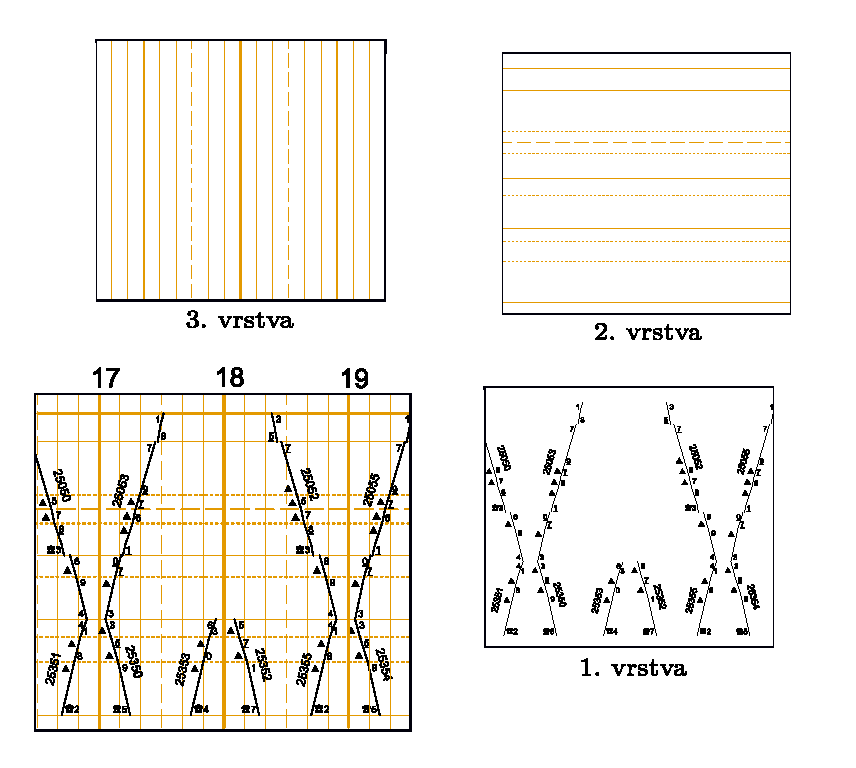
\includegraphics[width=\textwidth]{../img/kap2_drawing_layers}
	\caption{Možné rozdělení obsahu nákresného jízdního řádu na vrstvy}
	\label{fig:spec:njr_vrstvy}
\end{figure}

\begin{figure}[!htb]
	\centering					
	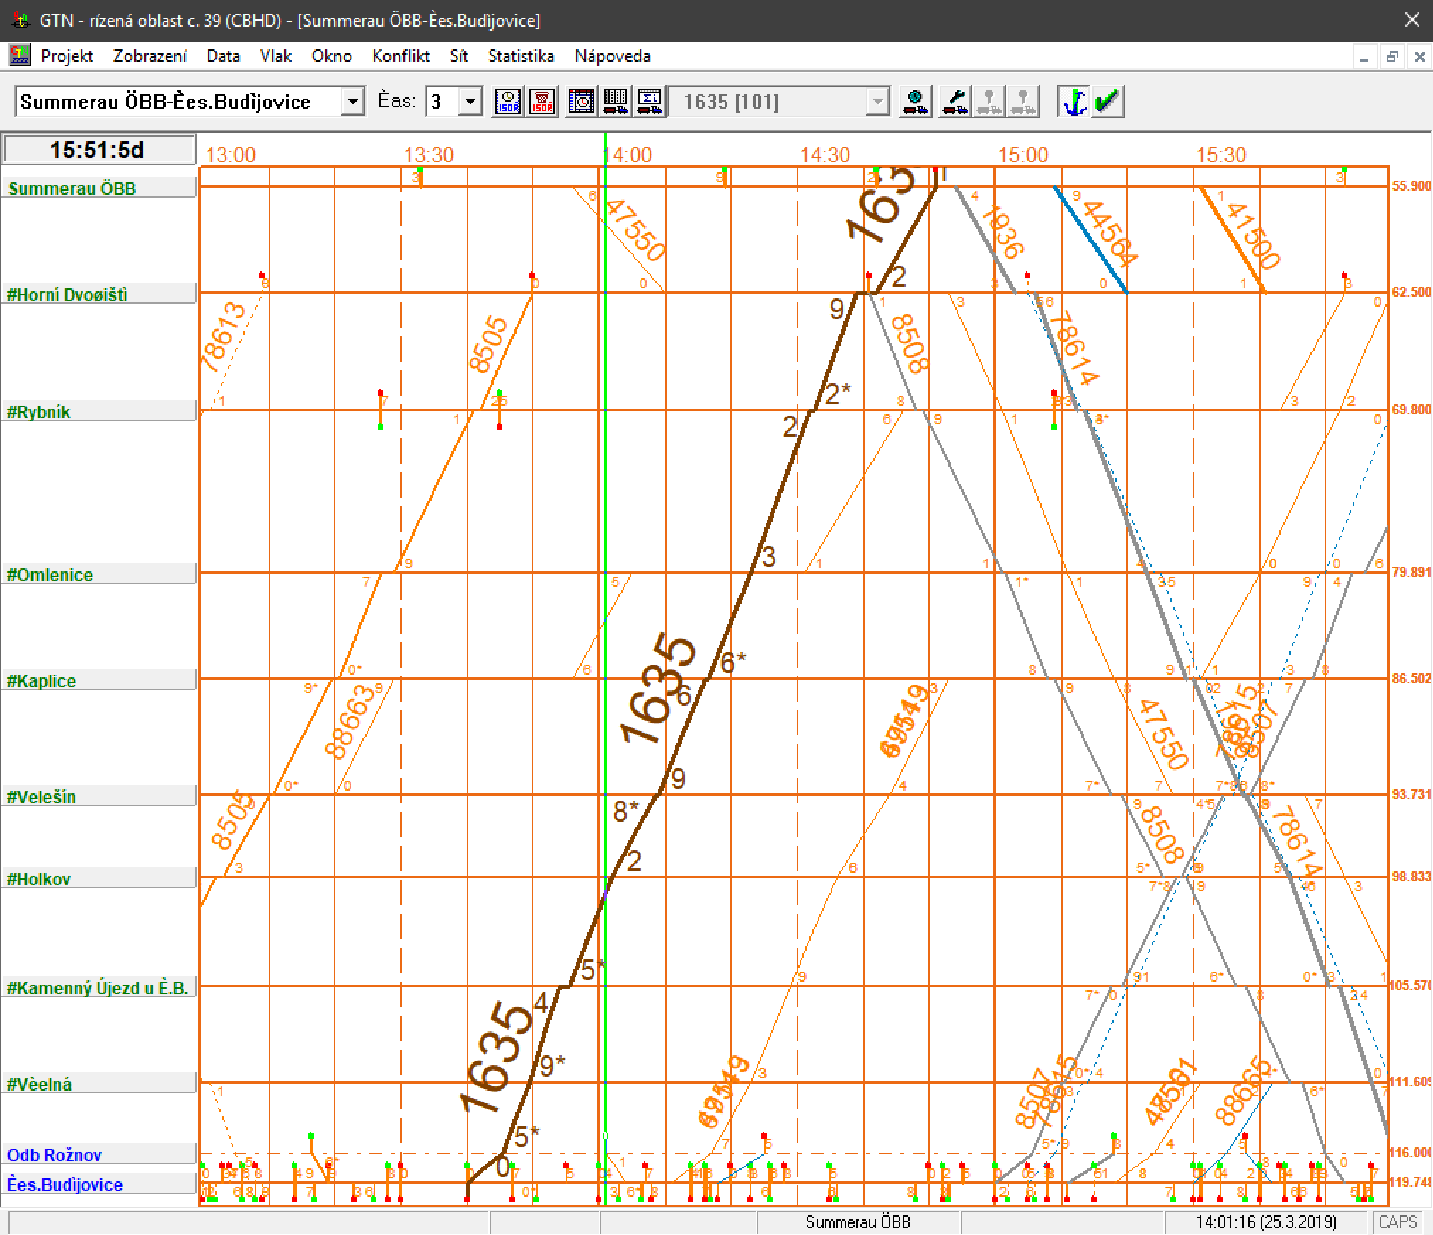
\includegraphics[width=0.7\textwidth]{../img/kap1_gtn_okno_interval_3h}
	\caption{Okno aplikace GTN s~vybraným vlakem vyneseným do popředí}
	\label{fig:spec:gtn_vrstva_vybrany_vlak}
\end{figure}

\newpage
\subsection*{Prvky nákresného jízdního řádu}
\label{kap2:view_elements}
Během změn zobrazení nákresného jízdního řádu je nutné jeho obsah pokaždé znovu vhodně rozmístit. Tento proces nazveme jako \textit{cyklus rozmístění}\footnote{layout cycle}. Pokud například zvětšíme výšku komponenty, zobrazovaný obsah se proporcionálně přerozmístí. Jelikož se změnou výšky změnil i~úhel sklonu šikmých čar, musí se znovu rozmístit prvky jako čísla vlaků nebo informace zobrazované v~ostrých úhlech. 

Některé implementace nákresných jízdních řádů můžou navíc obsahovat složitější konfigurace, které rozmístění komplikují. Dopravní bod například může být místo jedné horizontální čáry reprezentován souborem horizontálních čar, které odpovídají jeho kolejím. Zároveň je možné v~cyklu rozmístění vyhradit úseky kolem dopravních bodů, do kterých se mají umístit informace zobrazené v~ostrých úhlech. Všechny tyto prvky, které reprezentují nějakou část nákresného jízdního řádu a~je nutné je rozmístit, nazveme jako \textit{zobrazitelné prvky}. Základem pro rozmístění všech těchto prvků bude určení jejich velikosti, která může být nastavena různými způsoby, uvedených v~\ref{spec:zobrazitelne_prvky2}.

Pro jednoduchost implementace různých typů nákresných jízdních řádů tak chceme vývojářům umožnit co nejvíce obsahu, který je nutné rozmístit, systematicky popsat pomocí zobrazitelných prvků. S~obsahem nákresného jízdního řádu by pak bylo možné pracovat jako se strukturou stromu, jako na obrázku \ref{fig:prvky_mereni}.

\begin{enumerate}[label=\color{reqcolor}\textbf{R{\arabic*}},resume]
	\item \label{spec:zobrazitelne_prvky1} Obsah nákresného jízdního řádu je možné systematicky popsat strukturou prvků, které označíme jako \textit{zobrazitelné prvky}. Pomocí prvků je možné upravit zobrazení nákresného jízdního řádu v~závislosti na nastavení komponenty.
	\item \label{spec:zobrazitelne_prvky2} Implementace zobrazitelných prvků umožní konfigurovat jejich velikosti různými způsoby:		
\begin{enumerate}
	\item	Prvku může být přiřazena pevná velikost
	\item	Prvku je přiřazena jím požadovaná velikost
	\item	Prvku přiřazená velikost je závislá na nastavení komponenty
\end{enumerate}
 
\end{enumerate}

\begin{figure}[!hbt]
	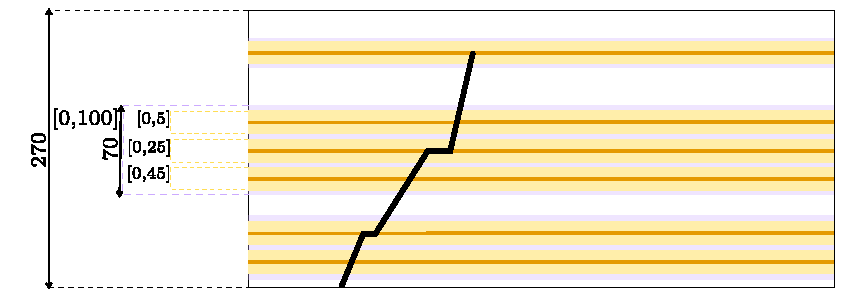
\includegraphics[width=\textwidth]{../img/kap2_infrastructure_layout}
	\caption{Rozdělení obsahu nákresného jízdního řádu do stromové struktury prvků zobrazení}
	\label{fig:prvky_mereni}
\end{figure}

\subsubsection*{Strategie rozmisťování zobrazitelných prvků}
\label{kap2:strategies_introduction}
Pro některé skupiny zobrazitelných prvků (informace v~ostrých úhlech nebo čísla vlaků) chceme, aby bylo možné vybrat specifické rozmístění, které nazveme \textit{strategií}. Výběr strategie ovlivňuje, kam a~jak moc přehledně se zobrazitelné prvky těchto skupin umístí. Každý typ nákresného jízdního řádu totiž umisťuje tyto zobrazitelné prvky jiným způsobem. Aplikace, s~kterými jsme se seznámili, preferují v~implementaci rozmístění jednoduchost, jelikož většina prostředků a~času strávených jejich vývojem byla určena na implementaci aplikační logiky a~složitější návrh grafické komponenty nebyl při návrhu aplikace zvažován. Knihovna by měla umožnit přehledné rozmisťování zobrazitelných prvků, jelikož se jedná o~vlastnost, která je důležitá pro uživatele aplikací při práci s~nákresným jízdním řádem. S~pomocí obrázku \ref{fig:spec:strategie_cisla_vlaku} si pro ilustraci uvedeme několik přístupů, které se můžou aplikovat při rozmisťování čísel vlaků.

\begin{itemize}
	\item Strategie (a) je nejjednodušší na implementaci. Její jednoduchost spočívá v~tom, že ve většině případů zobrazuje rozmístěné prvky dostatečně přehledně. Náhodně se vybere místo úseku mezi dopravními body, kam se má číslo vlaku umístit. Může ale dojít k~problému, kdy je úsek krátký a~číslo vlaku se bude překrývat s~kótou.
	\item Strategie (b) je dalším jednoduchým způsobem, jak prvky rozmístit přehledně. Strategie se snaží předejít překrývání čísla vlaku s~kótami. Číslo vlaku umístí na střed do nejdelšího dostupného úseku mezi dvěma sousedními dopravními body. Pokud se číslo do úseku nevejde, strategie ho dostatečně zmenší.
	\item Strategie (c) umisťuje číslo na rovnou aproximaci svislé čáry mezi více dopravními body, tak, aby se nepřekrýval s~kótami.
	\item Strategie (d) je použitelná v~případech, pokud vykreslujeme nákresný jízdní řád, který se nemění, jelikož je její implementace náročná na výpočet. Strategie podle složitějšího algoritmu může určit, jak se prvky do nákresného jízdního řádu vhodně rozmístí tak, aby se nepřekrývaly.
\end{itemize}

\begin{figure}[!htb]
	\centering					
	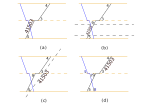
\includegraphics[width=\textwidth]{../img/kap2_strategies_train_numbers}
	\caption{Aplikovatelné strategie při rozmístění čísel vlaků}
	\label{fig:spec:strategie_cisla_vlaku}
\end{figure}

Naše knihovna by neměla mít pevně určené strategie, které se musí používat. Vývojář si tak může zvolit strategii, která mu přijde nejvíce vhodná. Není v~našich silách implementovat všechny možné strategie, ale můžeme knihovnu navrhnout tak, že zásadně ulehčí vytváření dalších strategií. 

Mělo by být možné v~rámci jedné strategie zobrazitelné prvky nahradit jinými, beze změny její implementace. Pro strategii totiž obecně není podstatné, s~jakými prvky pracuje. Všimněme si, že s~prvky pracuje jako s~obdélníky s~pevnou velikostí. Tento proces je zachycen na obrázku \ref{fig:pouziti_strategie}. Strategie nejdříve obdélník změří a~za pomoci operací škálování a~rotace obdélník vhodně umístí. Možnost oddělit strategii od konkrétních zobrazitelných prvků pak umožňuje pro více typů nákresných jízdních řádů použít již existující strategie na jejich specifické zobrazitelné prvky, jako je uvedeno na obrázku \ref{fig:spec:jine_rozmistitelne_prvky}.

\newpage
\begin{enumerate}[label=\color{reqcolor}\textbf{R{\arabic*}},resume]
	\item \label{spec:req:strategie1} Knihovna poskytne nástroje k~implementaci strategií, které rozmisťují zobrazitelné prvky do specifických míst jako ostré úhly nebo oblasti podél svislých čar
	\item \label{spec:req:strategie2} Strategie pracují se zobrazitelnými prvky jako s~obdélníky, jejichž zobrazení a~umístění je možné měnit:
	\begin{enumerate}
		\item Zobrazení prvku je možné strategií upravit transformací rotace
		\item Zobrazení prvku je možné strategií upravit transformací škálování
		\item Prvek je možné umístit na místo určené strategií
	\end{enumerate}
\end{enumerate}

\begin{figure}[!hbt]
	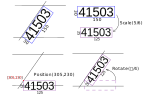
\includegraphics[width=\textwidth]{../img/kap2_strategy_application}
	\caption{Příklad aplikování strategie na zobrazitelný prvek}
	\label{fig:pouziti_strategie}
\end{figure}

\begin{figure}[!htb]
	\centering					
	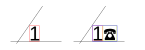
\includegraphics[width=.7\textwidth]{../img/kap2_view_elements_strategies}
	\caption{Možnost použít stejnou strategii na jiné zobrazitelné prvky}
	\label{fig:spec:jine_rozmistitelne_prvky}
\end{figure}

\pagebreak
\subsubsection*{Interakce se zobrazitelnými prvky a~hit-testy}
Jelikož by měla práce s~nákresným jízdním řádem nabízet co největší možnou úroveň interakce, chceme, aby bylo možné při práci s~komponentou pracovat interaktivně i~se zobrazitelnými prvky. Pokud by uživatel aplikace například klikl na kótu nebo prvek zobrazující složitější informace, nějaká jiná komponenta uživatelského rozhraní by na tuto událost mohla zareagovat a~zobrazit dodatečné informace doplňující vizualizaci v~nákresném jízdním řádu. Proces, kdy zjišťujeme, zda se nějaký bod nachází uvnitř rozmístěného geometrického útvaru, se nazývá \textit{hit-testování}.

\begin{enumerate}[label=\color{reqcolor}\textbf{R{\arabic*}},resume]
	\item \label{spec:req:hit-test1} Rozmístěné zobrazitelné prvky je možné otestovat, zda leží na konkrétním bodu plátna
	\item \label{spec:req:hit-test2} Na základě funkcionality \ref{spec:req:hit-test1} bude možné získat všechny zobrazitelné \linebreak prvky nacházející se na specifikovaném bodu plátna podle pořadí vykreslení 
\end{enumerate}

\subsubsection*{Kreslení zobrazitelných prvků}
Jedním ze složitých procesů, který bychom chtěli vývojářům ulehčit, je vykreslování zobrazitelných prvků. Pokud bychom vývojářům, kteří pracují na vykreslování zobrazitelných prvků, poskytli pouze plátno pro celý obsah nákresného jízdního řádu s~nástroji knihovny SkiaSharp, museli by sami do kreslení prvku zahrnout vzniklé transformace a~umístění prvku. Chtěli bychom, aby vývojáři mohli prvky vykreslovat způsobem, kdy by měl každý zobrazitelný prvek přidělené vlastní plátno na kreslení a~vykreslení by tak probíhalo nezávisle na zobrazení v~nákresném jízdním řádu.

\begin{enumerate}[label=\color{reqcolor}\textbf{R{\arabic*}},resume]
	\item \label{spec:zobrazitelne_prvky_vykresleni} Pro vykreslení obsahu zobrazitelného prvku je vytvořeno plátno, které odpovídá velikosti prvku. Vykreslení prvku tak probíhá nezávisle na celém zobrazení nákresného jízdního řádu.
\end{enumerate}

\subsection*{Základní model obsahu nákresných jízdních řádů}
\label{kap2:req:model_impl}
Jelikož nákresné jízdní řády mají mnoho společných vlastností, v~rámci splnění cíle \ref{uvod:cil:knihovna} \ref{uvod:cil:knihovna:ruzne_typy_njr} bychom chtěli vytvořit implementaci základního modelu nákresných jízdních řádů. Jejím rozšířením bude možné vytvořit konkrétní typ nákresného jízdního řádu. V~rámci základní implementace poskytneme vývojářům implementaci několika strategií.
\chapter{Analýza implementace knihovny GTTG}
Text této kapitoly podrobně analyzuje možné přístupy k~implementaci částí knihovny GTTG, aby byly splněny cíle \ref{uvod:cil:knihovna} \ref{uvod:cil:knihovna:ruzne_typy_njr} - \ref{uvod:cil:knihovna:dotnet_standard} uvedené na konci kapitoly \ref{kap:uvod} a~požadavky \ref{spec:req:interaction_trans1} - \ref{spec:zobrazitelne_prvky_vykresleni} uvedené v~kapitole \ref{kap:spec}.

\section[Implementace komponenty a~prostředí pro kreslení]{Implementace komponenty a~prostředí pro kreslení}
\label{kap:impl:komp}
Jedním z~cílů pro vývoj knihovny je zajistit její integrovatelnost do aplikací ~(cíl \textbf{\color{goalcolor}G1}\ref{uvod:cil:knihovna:integrace_do_aplikaci}). Toho dosáhneme pomocí správné implementace komponenty. Jelikož knihovna SkiaSharp bude při určování implementace komponenty a~integrace knihovny do aplikací hrát zásadní roli, nejdříve se před samotným rozborem implementace seznámíme s~jejími základními principy fungování.

\subsection{Úvod do práce s~knihovnou SkiaSharp} 
Základem pro kreslení v~knihovně SkiaSharp je třída \texttt{SKCanvas}, která představuje plátno pro kreslení. Mezi instanční metody této třídy patří kreslící příkazy (například \texttt{DrawText()}, \texttt{DrawCircle()}), které se na základě dodaných parametrů nanáší na plátno. Jelikož je knihovna SkiaSharp 2D, pořadí nanášení příkazů na plátno je určeno pořadím volání metod. Kreslení na plátno, vzniklé jako výsledek aplikování několika kreslících příkazů na následujícím fragmentu kódu, je uvedeno na obrázku \ref{fig:skia_kresleni_ukazka}.

\begin{csharpcode}
var paint = new SKPaint {Color = SKColors.Green, Style = SKPaintStyle.Fill};
canvas.DrawRect(SKRect.Create(x: 145, y: 10, width: 75, height: 30), paint);
paint.Color = SKColors.BlueViolet;
canvas.DrawCircle(new SKPoint(x: 70, y: 70), radius: 25, paint: paint);
\end{csharpcode}

\begin{figure}[!hbt]
	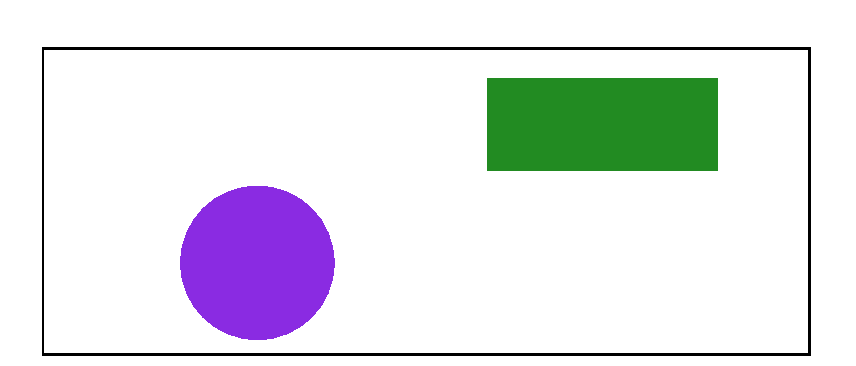
\includegraphics[width=\textwidth]{../img/kap3_skia_matrix_identity}
	\caption{Kreslení na plátno odpovídající kreslícím příkazům v~předchozím fragmentu kódu}
	\label{fig:skia_kresleni_ukazka}
\end{figure}

\subsubsection*{Transformace kreslících příkazů}
\label{kap3:skia_intro_transformations}
Plátno \texttt{SKCanvas} je možné konfigurovat přenastavením matice označované jako \texttt{transform matrix} a~výřezu plátna, který se nazývá \texttt{clip}. Část kreslícího příkazu, který se nachází mimo \texttt{clip}, se nevykreslí. Nastavení \texttt{transform matrix} ovlivňuje výsledek kreslících příkazů. Na obrázku \ref{fig:skia_kresleni_ukazka_transformace} se na plátno aplikovaly stejné příkazy jako při kreslení na obrázku \ref{fig:skia_kresleni_ukazka}, pouze se před jejich aplikací nastavila \texttt{transform matrix} na následujícím fragmentu kódu. Obsah výkresu je nyní transformován rotací o~$\pi$/8 po směru hodinových ručiček se středem v~levém horním rohu zeleného obdélníku.

\begin{csharpcode}
var pivotX = 145; var pivotY = 10;
SKMatrix.Rotate(ref matrix, (float) Math.PI / 8, pivotX, pivotY);
canvas.SetMatrix(matrix);
\end{csharpcode}

\begin{figure}[!hbt]
	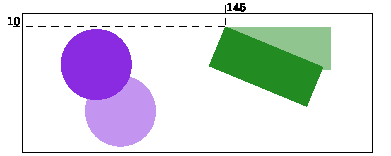
\includegraphics[width=\textwidth]{../img/kap3_skia_matrix_translate_scale}
	\caption{Výkres \ref{fig:skia_kresleni_ukazka} se změněnou \texttt{transform matrix}. Původní výkres je pro porovnání uveden ve stínu}
	\label{fig:skia_kresleni_ukazka_transformace}
\end{figure}

Konfigurace \texttt{transform matrix} se vykonává voláním \texttt{SetMatrix()}, \texttt{clip} se aplikuje vzhledem k~současné \texttt{transform matrix} například pomocí \texttt{ClipRect()}. \texttt{Transform matrix} i~\texttt{clip} je možné efektivně měnit a~vracet do původních stavů, jelikož konfigurace jsou plátnem ukládány na jeho zásobník modifikací. Pro každou sérii kreslících příkazů je tak možné použít jinou transformaci.

\subsubsection*{Sestrojení plátna}
Pokaždé, když chceme pracovat s~knihovnou SkiaSharp, musíme pro kreslení získat instanci plátna \texttt{SKCanvas}. Plátno může být sestrojeno nad existující bitmapou nebo může být vytvořeno jako instanční proměnná třídy \texttt{SKSurface}, která je zodpovědná za práci s~nástrojem poskytující pixely, na které \texttt{SKCanvas} kreslí. Je tak možné rozhodnout, jestli jsou pixely alokovány v~paměti nebo GPU. Dále je možné, aby SkiaSharp vykreslovala obsah plátna do PDF nebo jako vektorovou grafiku v~SVG. Jednou z~vlastností \texttt{SKCanvas} i~\texttt{SKSurface} je, že po vytvoření již nemůžou měnit svou velikost.

\newpage
\subsubsection*{Podpora v~rámci uživatelských rozhraní}
\label{kap3:skia_ui_elements}
Knihovna SkiaSharp nabízí pro některé GUI frameworky implementaci prvku uživatelského rozhraní, jehož plocha se používá jako plátno \texttt{SKCanvas}.
To přináší vývojářům zásadní ulehčení jejich práce, jelikož prvek sám sestrojí \texttt{SKSurface} a~při změně velikosti prvku vytvoří nový s~upravenou velikostí. Kdykoliv, když je vizualizace prvku invalidována, je obnoven kreslící cyklus, v~kterém vývojář pracuje s~plochou prvku uživatelského rozhraní jako s~\texttt{SKCanvas}. Vývojáři díky těmto implementacím nemusí pracovat s~kreslícím \textit{backendem}, který by museli zapojit do \texttt{SKSurface} za poskytnutí mnoha parametrů popisující jeho nastavení.

\subsection{Integrace knihovny do aplikací}
Na základě zmíněných vlastností knihovny SkiaSharp si nyní popíšeme, jak naše knihovna bude integrována do aplikací. V~rámci této integrace je nutné určit, jaké nástroje musí vývojář knihovně dodat.

\subsubsection*{Reprezentace jednotek pixelů}
\label{kap3:jednotky_pixelu}
V~rámci implementace komponenty můžeme splnit požadavky \ref{spec:req:unit1} a~\ref{spec:req:unit2} související s~existencí plátna v~různých jednotkách pixelů. Uvedli jsme si, že \linebreak SkiaSharp nabízí implementaci UI prvků určených pro kreslení. U~těchto prvků je možné nastavit jednotky pixelů plátna \texttt{SKCanvas}. V~prvku \texttt{SKElement} GUI frameworku WPF se jednotky pixelů nastavují vlastností \texttt{IgnorePixelScaling} uvedené na následujícím fragmentu kódu.

\begin{csharpcode}
public class SKElement : FrameworkElement {

/// <summary>
/// Gets or sets a~value indicating whether the drawing canvas
/// should be resized on high resolution displays.
/// </summary>
/// <remarks>
/// By default, when false, the canvas is resized to 1 canvas
/// pixel per display pixel. When true, the canvas is resized to device
/// independent pixels, and then stretched to fill the view. Although
/// performance is improved and all objects are the same size on different
/// display densities, blurring and pixelation may occur.
/// </remarks>  
public bool IgnorePixelScaling {
\end{csharpcode}

Komentář vysvětluje, že pokud pixely plátna \texttt{SKCanvas} odpovídají pixelům nezávislých na zařízení, je dodána \texttt{SKSurface} bitmapa v~jednotkách pixelů s~DPI 96, které odpovídá ve WPF jednotkám pixelů nezávislých na zařízení. Bitmapa pak pro každý takový pixel může v~závislosti na zařízení použít několik fyzických pixelů.

Pokud bychom řešili tento problém obecně, plátno by bylo vytvořeno ve velikosti odpovídající ploše prvku v~jednotkách pixelů zařízení a~více pixelů zařízení by mohlo odpovídat jednomu pixelu nastavením škálování v~\texttt{transform matrix} plátna. Pokud bychom velikost komponenty určovali pomocí velikosti plátna \texttt{SKCanvas}, nastala by tímto způsobem nekonzistence v~reprezentaci velikostí -- v~případě nastavení \texttt{IgnorePixelScaling} je plátno udáváno v~konečné velikosti pixelů nezávislých na zařízení a~v~případě nyní zmiňovaného způsobu by odpovídalo velikosti pixelů zařízení, ačkoliv v~obou případech chceme v~komponentě pracovat s~jednotkami pixelů nezávislých na zařízení. I~přes tyto nevýhody bychom chtěli takovou konfiguraci umožnit. 

Rozhodli jsme se proto, že velikost komponenty bude explicitně uváděna jiným způsobem a~s~velikostí \texttt{SKCanvas} knihovna pracovat nebude. Vývojář, který bude chtít použít zvětšování pomocí \texttt{transform matrix}, sám matici nastaví a~knihovna mu tuto konfiguraci nezmění. Protože existují různé způsoby, jak můžou být pro \texttt{SKSurface} alokovány pixely, nechceme v~knihovně vytvářet nové plátno v~bitmapě a~budeme po vývojáři požadovat, aby dodal vlastní \texttt{SKSurface} \linebreak s~\texttt{SKCanvas}. Jiná implementace by byla neefektivní vzhledem k~možnostem\linebreak knihovny SkiaSharp. Zároveň požadujeme, aby vývojář provedl všechna doposud popisovaná nastavení sám mimo knihovnu. Pokud se komponentě předávají body z~plochy prvku, která pracuje s~jinými jednotkami pixelů, vývojář musí převod jednotek sám implementovat. Jelikož už vývojář v~této konfiguraci pracuje s~hodnotou DPI, která je uvedena v~požadavku \ref{spec:req:unit2}, hodnotu DPI komponentě nastaví sám. Všechny tyto konfigurace se tak odehrávají na stejné úrovni a~knihovna bude konzistentně pracovat se stejnými jednotkami velikosti.

\subsection{Reprezentace časových intervalů}
Musíme najít způsob, jak reprezentovat časové intervaly definované \ref{spec:req:int1} a~\ref{spec:req:int2}. Zároveň \ref{spec:req:conv1} požadujeme, aby bylo možné časové údaje používané v~reprezentaci intervalů převádět do bodů plátna. Převod by měl být co nejméně komplikovaný. Doposud jsme si uváděli situace, kdy časový interval nepřesáhne několik hodin a~proto by se nabízelo použít k~reprezentaci časových údajů struktury, které reprezentují pouze čas, ale neobsahují už informaci o~datu. Každá aplikace ale pracuje s~jinou reprezentací časových údajů v~jejím modelu dat. Existují aplikace, které sledují současný provoz a~v~časových údajích zahrnují i~datum.

K~reprezentaci časových údajů v~knihovně jsme se proto rozhodli použít strukturu \texttt{DateTime}. Převod jiných struktur pracujících s~časovými údaji do hodnot \texttt{DateTime} není komplikovaný a~převod v~rámci \ref{spec:req:conv1} je přímočarý -- rozdíl konce a~začátku intervalu vytvoří strukturu \texttt{TimeSpan} obsahující hodnotu \texttt{TotalMilliseconds}, s~jejíž násobky jde dále při převodu pracovat. Při použití data i~času nemůže docházet k~nejednoznačnostem při porovnávání a~převodu časových intervalů.

\subsection{Modifikace komponenty}
\label{kap3:modifikace_komponenty}
Modifikace komponenty jako translace nebo škálování nesmí překročit ohraničení definované \ref{spec:req:interaction_trans1}. Jelikož se chybné modifikace mohou při interakci uživatele s~komponentou vyskytovat běžně, nechceme, aby vyhazovaly výjimky. Zároveň ale chceme vývojáře informovat o~úspěšnosti modifikace, jelikož na jejím provedení může být například závislé vykreslení obsahu a~nechceme zbytečně vykreslovat modifikací nezměněný obsah. Rozhodli jsme se, že každé volání modifikace bude mít jako návratovou hodnotu výčtový typ, který bude poskytovat informace o~úspěšnosti modifikace. Na následujícím fragmentu kódu je příklad takového výčtového typu pro modifikaci \ref{spec:req:interaction_zoom1} škálující zobrazení:

\begin{csharpcode}

public enum ScaleTransformationResult {
    ViewModifiedWithTransformedOrigin,
    ViewModifiedWithSameOrigin,
    ViewUnmodified
}

public ScaleTransformationResult TryScale(SKPoint origin, float delta) {
	/*...*/
}
\end{csharpcode}

Pro případ, kdy nastane stav \ref{spec:req:interaction_zoom2} a~pohled by se vyskytl mimo ohraničení \ref{spec:req:interaction_trans1}, je vrácen \texttt{ViewModifiedWithTransformedOrigin}. Rozhodli jsme se, že se pohled v~rámci volání \texttt{TryScale()} deterministicky upraví tak, aby byl posunut o~délku, kterou v~ohraničení překračuje. V~případě, že faktor škálování je menší než jedna, je vrácen \texttt{ViewUnmodified}.

\subsubsection*{Práce s~komponentou ve vícevláknovém prostředí}
Může docházet k~případům, kdy vývojář bude ke knihovně přistupovat z~více vláken. Například je v~rámci aplikace spuštěn periodický časovač, který běží v~dalším vlákně a~opakovaně upravuje nějakou část komponenty, aby odpovídala modelu dat v~aplikaci. Pokud by se taková změna stavu komponenty z~jiného vlákna vyskytla během vykreslování nebo jiných změn v~komponentě, může se vyskytnout chybový stav označovaný jako \textit{race condition}. Chceme určit postup, jak systematicky těmto problémům předcházet. Jelikož knihovna bude obvykle součástí uživatelských rozhraní, která řeší podobné problémy pro jejich prvky, nabízí se jejich řešení rozšířit i~na naší knihovnu. Každé uživatelské rozhraní definuje svá pravidla pro práci ve vícevláknovém prostředí označovaná jako \textit{threading model}. Většinou je pravidlem povolovat u~každého prvku změnu jeho stavu pouze z~vlákna, které se nazývá \textit{UI vlákno}. Kdykoliv uživatel změní stav prvku z~jiného vlákna, je vyhozena výjimka. Práci z~jiného vlákna modifikující stav prvku je však možné zařadit do UI vlákna přes strukturu obecně nazývanou \textit{dispatcher}. Takto je řešena synchronizace na úrovni prvků uživatelského rozhraní. Například v~GUI frameworku WPF je každý UI prvek potomkem abstraktní třídy \texttt{DispatcherObject}, která nabízí nástroje pro ověření přístupu přes metody uvedené na následujícím fragmentu kódu. Při nastavování vlastností prvků uživatelského rozhraní se pak kontroluje přístup v~rámci volání \texttt{SetValue()} a~metody přístup kontrolují přes \texttt{VerifyAccess()}.

\begin{csharpcode}
public abstract class DispatcherObject {

	public void VerifyAccess() {
      this._dispatcher?.VerifyAccess();
    }

	public void SetValue(DependencyProperty dp, object value) {
      this.VerifyAccess();
\end{csharpcode}

Pokud bychom se rozhodli řešit tento problém na úrovni knihovny, museli bychom najít řešení, které bude jednoduché na implementaci a~zajistí konzistentní chování při práci s~celým obsahem knihovny. Nemůžeme převzít žádné konkrétní řešení, které existuje v~rámci nějakého GUI frameworku, jelikož jedním z~cílů je zajistit přenositelnost knihovny na úrovni .NET Standard (cíl \textbf{\color{goalcolor}G1}\ref{uvod:cil:knihovna:dotnet_standard}). Mohli bychom implementovat vlastní řešení, které by se chovalo podobně jako zmíněný \texttt{DispatcherObject} a~dispatcher, ale zajistit jeho správnost i~udržitelnost by bylo náročné. Nalezením řešení na úrovni knihovny bychom také způsobili zpomalení aplikací, které budou ke kódu knihovny přistupovat z~jednoho vlákna. Z~těchto důvodů jsme se rozhodli, aby vývojář řešil problémy synchronizace na úrovni uživatelského rozhraní s~nástroji, které GUI frameworky nabízí. Následující fragment kódu z~vlákna běžícího vedle UI vlákna v~aplikaci ve WPF zařadí do UI vlákna přes \texttt{Dispatcher.Invoke()}  vykonání lambda funkce, která přidá nový vlak do modelu vykreslovaného komponentou.

\begin{csharpcode}
Train newTrain = /*...*/;

Dispatcher.Invoke(() => {
	Model.Trains.Add(newTrain);
});
\end{csharpcode}

\subsection{Reprezentace plátna v~knihovně}
\label{fig:analyza_impl:platno}
Podle požadavku \ref{spec:req:canvas1} chceme vývojářům poskytnout plátno nákresného jízdního řádu, které má být nastaveno tak, aby v~komponentě byl zobrazen jeho výřez v~závislosti na jejím stavu. Toto plátno nazveme \texttt{ContentCanvas}. Implementaci jeho nastavení v~komponentě se nyní budeme věnovat.

Pro vykreslení správného výřezu plátna \texttt{ContentCanvas} můžeme nastavit \texttt{transform matrix} na plátně \texttt{SKCanvas}, které podle \ref{kap3:jednotky_pixelu} knihovně dodává vývojář k~vykreslení. V~počátečním stavu zobrazeném na obrázku \ref{fig:impl:platno_matice_identity} je \texttt{transform matrix} identita. Modifikace komponenty popsaná \ref{spec:req:interaction_trans2} odpovídá operaci translace, \ref{spec:req:interaction_zoom1} odpovídá škálování. Upravená \texttt{transform matrix} po modifikaci posunem je zobrazena na obrázku \ref{fig:impl:platno_matice_transformace}. Bod [300,300] na \texttt{ContentCanvas} se nyní mapuje na [0,0] a~vykreslí se na levém horním rohu komponenty. 

\begin{figure}[h]
\centering
\begin{subfigure}{0.45\textwidth}
	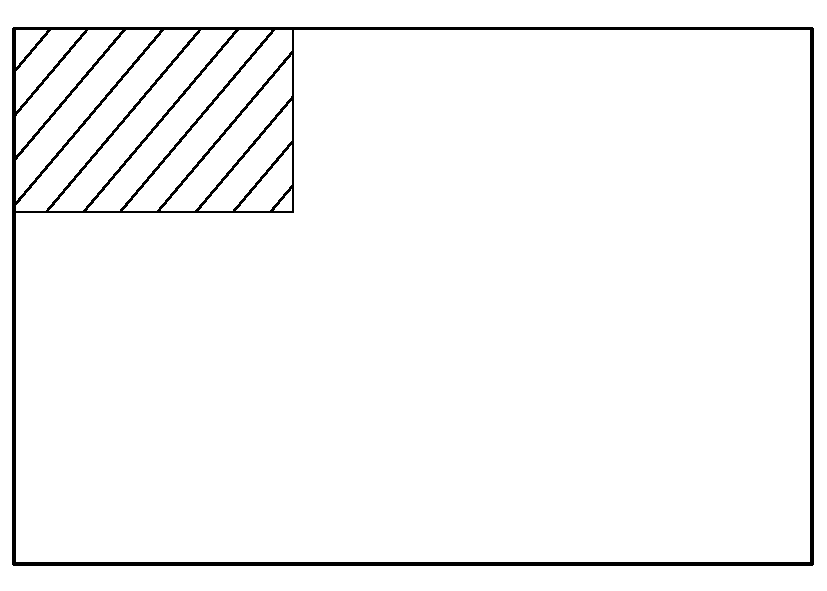
\includegraphics[width=\linewidth]{../img/kap3_komponenta_identita}
	\centering

$\begin{pmatrix}
1 & 0 & 0 \\
0 & 1 & 0 \\
0 & 0 & 1
\end{pmatrix}$

	\caption{Identita}
	\label{fig:impl:platno_matice_identity}
\end{subfigure}
\begin{subfigure}{0.45\textwidth}
	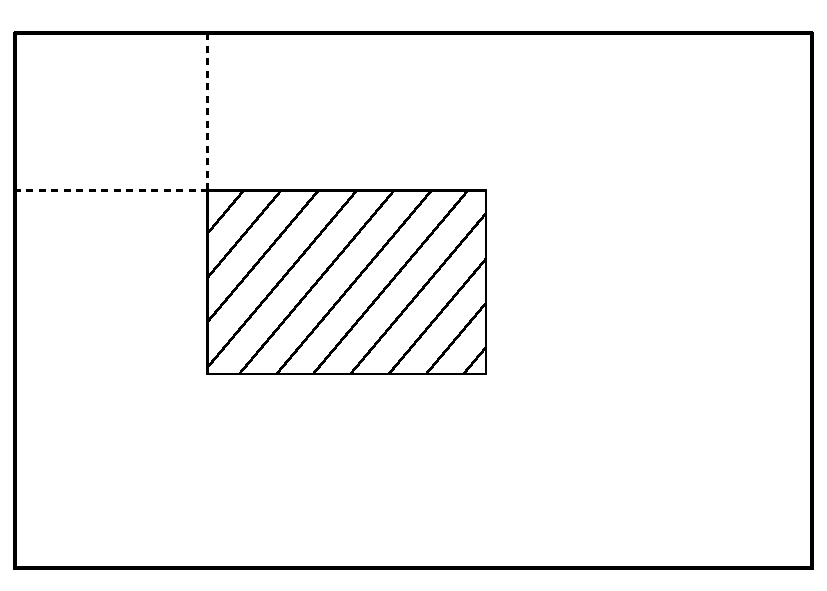
\includegraphics[width=\linewidth]{../img/kap3_komponenta_translace}
\centering
$\begin{pmatrix}
1 & 0 & 0 \\
0 & 1 & 0 \\
-300 & - 300 & 1
\end{pmatrix}$

	\caption{Translace}
	\label{fig:impl:platno_matice_transformace}
\end{subfigure}
\end{figure}

\newpage
Nastavení \texttt{transform matrix} plátnu \texttt{SKCanvas} pomocí \texttt{SetMatrix()} se \linebreak v~knihovně Skia v~tomto případě optimalizuje -- její implementace je schopna zjistit, že nastavovaná matice odpovídá matici posunu a~při následujícím aplikování kreslících příkazů neproběhne obecná transformace násobením s~nastavenou maticí, ale pouze se k~bodům kreslícího příkazu přičte po osách délka posunu. Protože jiná implementace by byla neefektivní vzhledem k~možnostem knihovny Skia, rozhodli jsme se výřez nastavit tímto způsobem.

\subsubsection*{Vykreslování obsahu mimo zobrazovanou oblast v~komponentě}
\label{kap3:view_element_bounding_check}
Ve dvou bodech si uveďme, jaké výhody pro vývojáře knihovny přináší používání plátna \texttt{ContentCanvas}:

\begin{enumerate}
	\item \label{impl:njr_platno_vyhody_kresleni} Pro vývojáře se oddělil proces zobrazení obsahu komponenty od vykreslení obsahu nákresného jízdního řádu. Díky používání \texttt{ContentCanvas} vývojář nemusí počítat, jaký jeho výřez se v~komponentě zobrazí a~může vykreslit celý obsah nezávisle na tomto zobrazení.
	\item \label{impl:njr_platno_vyhody_rozmisteni} Výpočet, v~němž se rozmístí obsah zobrazený v~komponentě a~který jsme nazvali \textit{cyklem rozmístění}, probíhá pro celý obsah plátna \texttt{ContentCanvas}. Cyklus rozmístění musí probíhat v~případě změny velikosti komponenty. Modifikace měnící zobrazovaný výřez v~komponentě s~cyklem rozmístění nesouvisí.
\end{enumerate}

Používání plátna \texttt{ContentCanvas} může vedle těchto výhod představovat výkonnostní problém. Na obrázku \ref{fig:platno_mimo_komponentu} se nachází šedě podbarvená část jeho obsahu, která se v~komponentě nezobrazí a~přesto se vykresluje. Ušetřený čas za nehledání zobrazovaného obsahu tak může být převážen vykonáním kreslících příkazů, které se nezobrazí.

\begin{figure}[!bht]
	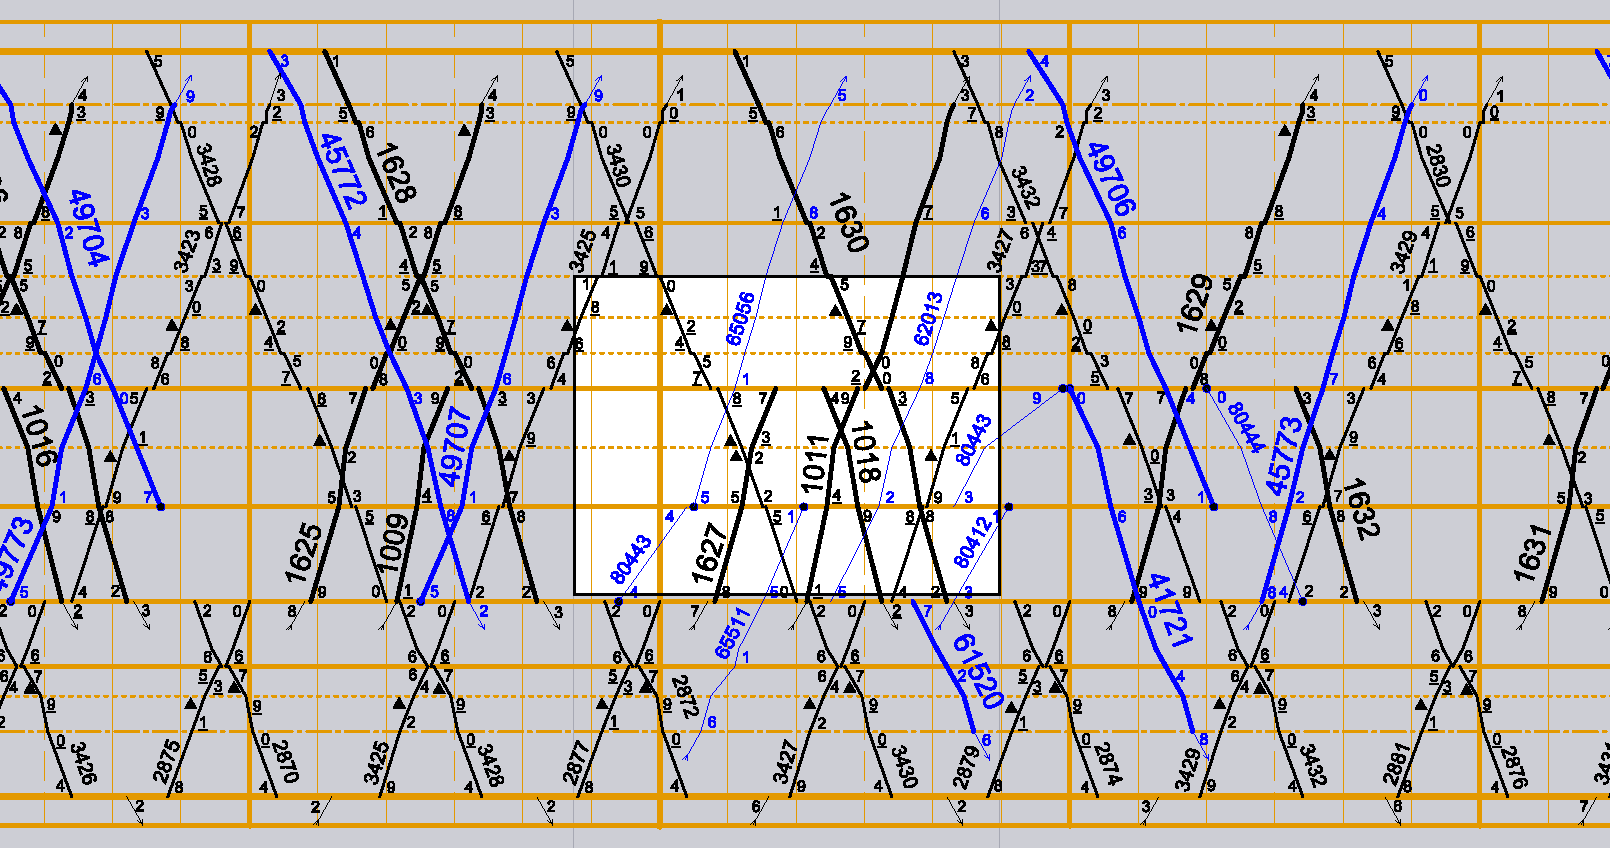
\includegraphics[width=\textwidth]{../img/kap3_platno_mimo_komponentu}
	\caption{Šedě podbarvený obsah \texttt{ContentCanvas} nacházející se mimo zobrazení komponenty}
	\label{fig:platno_mimo_komponentu}
\end{figure}

Hledání zobrazovaného obsahu budeme místo vývojáře řešit na úrovni \linebreak knihovny efektivní metodou, která je založena na následujícím pozorování. Podívejme se, na jaký obsah \texttt{ContentCanvas} se používá nejvíce kreslících příkazů. Souřadnicová síť jako několik čar nepředstavuje pro kreslení zásadní problém, stejně tak i~lomené čáry znázorňující průběh jízdy vlaků. Ke každému vlaku ale existuje několik zobrazitelných prvků, které často obsahují pro kreslení složitý obsah, jakým je například text. Na obrázku \ref{fig:prvky_mimo_komponentu} jsme v~části obsahu, která se v~komponentě nezobrazí, ohraničili zobrazitelné prvky červenými obdélníky.

\begin{figure}[!hbt]
	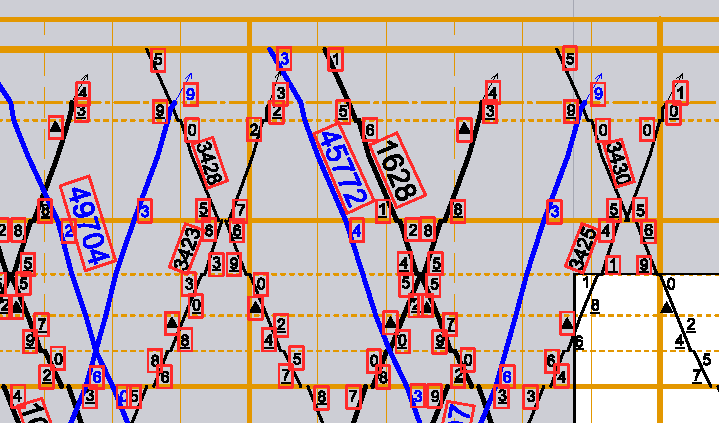
\includegraphics[width=\textwidth]{../img/kap3_zobrazitelne_prvky_mimo_komponentu}
	\caption{Zobrazitelné prvky označené červenými obdélníky se nacházejí mimo zobrazení komponenty}
	\label{fig:prvky_mimo_komponentu}
\end{figure}

Toto pozorování nyní spojíme s~prací se zobrazitelnými prvky v~rámci cyklu rozmístění. Strategie, které jsme si představili v~\ref{kap:spec:obsah_njr}, v~cyklu rozmístění pracují se zobrazitelnými prvky jako s~obdélníky, které někam umístí a~transformacemi rotací a~škálování je upraví. Tyto obdélníky odpovídají červeným obdélníkům na obrázku \ref{fig:prvky_mimo_komponentu}. Jelikož probíhá cyklus rozmístění na celém obsahu, jsou všechny zobrazitelné prvky před vykreslením již rozmístěny a~obdélníky je tak možné určit. Zobrazitelný prvek vykreslíme pouze v~případě, pokud se část jeho obdélníku nachází v~komponentě.

Nalezli jsme řešení, které je založeno na existující implementaci knihovny a~vzniká jako vedlejší výsledek rozmístění zobrazitelných prvků v~cyklu rozmístění. Kreslení obsahu tak zabere méně času než v~případě, kdy se vykreslí celý obsah nebo když by vývojář používal své vlastní řešení pro hledání zobrazeného obsahu v~komponentě.
\newpage
\section{Práce s~obsahem nákresného jízdního řádu}
V~této části určíme, jak implementovat knihovnu tak, aby umožnila tvorbu různých typů nákresných jízdních řádů (cíl \textbf{\color{goalcolor}G1}\ref{uvod:cil:knihovna:ruzne_typy_njr}) a~byly splněny požadavky kapitoly \ref{kap:spec}, které souvisí s~prací s~obsahem nákresného jízdního řádu.

\subsection{Implementace zobrazitelných prvků}
\label{kap3:zobrazitelne_prvky}
Zobrazitelným prvkům chceme v~cyklu rozmístění podle \ref{spec:zobrazitelne_prvky2} přidělovat různými způsoby jejich velikost. S~velikostí a~umístěním prvku pracují požadavky \textit{hit-testování} \ref{spec:req:hit-test1}, vykreslování \ref{spec:zobrazitelne_prvky_vykresleni} a~umístění do strategií \ref{spec:req:strategie2}. Před zvážením možné implementace cyklu rozmístění prvků určíme, jak na ní bude závislá implementace těchto požadavků.

\subsubsection*{Vykreslení zobrazitelných prvků}
\label{kap3:vykresleni_zobrazitelnych_prvku}
Pro vykreslování zobrazitelných prvků chceme vývojářům podle \ref{spec:zobrazitelne_prvky_vykresleni} předávat vlastní plátno, které bude odpovídat velikost prvku. V~podkapitole \ref{kap3:jednotky_pixelu} jsme se rozhodli, že knihovna bude pracovat pouze s~jedním plátnem -- \texttt{SKCanvas} poskytnutým vývojářem. Plátno pro zobrazitelný prvek tak bude představovat vytvoření pohledu na toto plátno, podobně jako \texttt{ContentCanvas}, jehož pohled jsme nastavili pomocí \texttt{transform matrix}. Na základě výhod uvedených v~\ref{fig:analyza_impl:platno} jsme se také rozhodli pro vykreslení plátna zobrazitelných prvků nastavit \texttt{transform matrix}. Hodnoty této matice budou závislé na umístění prvku na \texttt{ContentCanvas} a~\texttt{transform matrix} plátna \texttt{ContentCanvas}. Umístění prvku budeme reprezentovat maticí, kterou nazveme \texttt{placement matrix} a~abychom získali \texttt{transform matrix} prvku, vynásobíme ji s~\texttt{transform matrix} plátna \texttt{ContentCanvas}. Obrázek \ref{fig:matice_umisteni1} obsahuje zobrazitelný prvek, pro nějž tuto matici vypočítáme.
\begin{figure}[!bht]
	\centering
	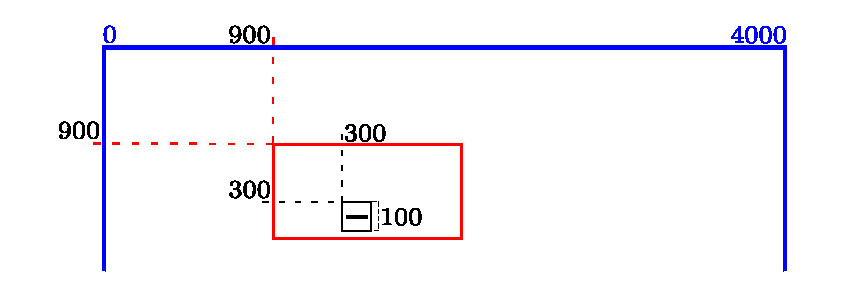
\includegraphics[width=0.75\textwidth]{../img/kap3_matice_umisteni.pdf}
	\caption{Příklad zobrazitelného prvku v~komponentě a~plátně \texttt{ContentCanvas}}
	\label{fig:matice_umisteni1}
\end{figure}
\begin{figure}[!bht]

\centering 
$\color{blue}
\begin{pmatrix} 
1 & 0 & 0 \\
0 & 1 & 0 \\
-900 & -900 & 1
\end{pmatrix}$
\color{black}
$\times$
\color{red} 
$\begin{pmatrix} 
1 & 0 & 0 \\
0 & 1 & 0 \\
1200 & 1200 & 1
\end{pmatrix}$
\color{black}
$=$
$\begin{pmatrix} 
1 & 0 & 0 \\
0 & 1 & 0 \\
300 & 300 & 1
\end{pmatrix}$
\caption{Výpočet \texttt{transform matrix} zobrazitelného prvku pomocí modré \texttt{transform matrix} plátna \texttt{ContentCanvas} a~červené \texttt{placement matrix}}
\end{figure}
\newpage
Podle \ref{spec:req:strategie2} chceme navíc zobrazení modifikovat rotací a~škálováním v~rámci strategií. Tyto transformace pak budou zaznamenány v~\texttt{placement matrix}. \linebreak K~násobení bychom mohli použít obecné maticové násobení implementované knihovnou SkiaSharp, které se ale provolává do C++ kódu knihovny Skia. Jelikož ale pracujeme pouze s~maticovými operacemi rotace, posunu a~škálování, můžeme násobit pouze některé prvky matic. Na následujícím fragmentu kódu je výsledná operace vytvářející \texttt{transform matrix} prvku, která zabere pouze šest násobení. 

\begin{csharpcode}
var canvasScaleX = canvasTransformMatrix[0]; 
var canvasScaleY = canvasTransformMatrix[4];
var canvasTransX = canvasTransformMatrix[2];
var canvasTransY = canvasTransformMatrix[5];

/* Other indices set to 0 */
var elementTransformMatrix = new SKMatrix { 
	/*A[3,3]*/ Persp2 = 1,
	/*A[1,1]*/ ScaleX = placementMatrix.ScaleX * canvasScaleX,
	/*A[1,2]*/ SkewY = placementMatrix.SkewY * canvasScaleY,
	/*A[2,1]*/ SkewX = placementMatrix.SkewX * canvasScaleX,
	/*A[2,2]*/ ScaleY = placementMatrix.ScaleY * canvasScaleY,
	/*A[3,1]*/ TransX = placementMatrix.TransX * canvasScaleX 
					    + canvasTransX,
	/*A[3,2]*/ TransY = placementMatrix.TransY * canvasScaleY 
						+ canvasTransY
};
\end{csharpcode}

Cyklus rozmístění zobrazitelného prvku bude muset pro výpočet matice \linebreak \texttt{placement matrix} prvku nastavit jeho umístění na \texttt{ContentCanvas} a~jeho hodnoty škálování a~rotace při transformaci strategií.

\subsubsection*{Vliv strategií na cyklus rozmístění}
Podle požadavku \ref{spec:zobrazitelne_prvky2} chceme zobrazitelné prvky strategiemi transformovat operacemi škálování a~rotace. Transformace může mít dopad pouze na vykreslení prvku nebo může změnit i~jeho velikost. Operace škálování by například mohla prvku proporcionálně přidělit jinou velikost a~prvek by na změnu reagoval. Měnila by se tak i~velikost plátna pro prvek a~zároveň s~ní i~umístění jeho kreslících příkazů. Taková implementace neodpovídá původnímu záměru prvky vykreslovat pokud možno nezávisle na zobrazení. Proto jsme se rozhodli transformace implementovat tak, aby strategie prvky pouze vizuálně transformovaly pomocí \texttt{placement matrix}. Během transformací se ale mění i~umístění prvků, pokud má prvek potomky. Cyklus rozmístění pak bude muset pro celý strom prvků při rotaci přepočítat umístění prvků a~jejich hodnoty pro výpočet \texttt{placement matrix}.

\subsubsection*{Umístění prvků na plátně}
\label{kap3:element_hit_test}
Podle \ref{spec:req:hit-test1} chceme dokázat zjistit, zda se nějaký bod plátna \texttt{ContentCanvas} nachází v~zobrazitelném prvku umístěném na tomto plátně. Jelikož můžou být prvky transformovány rotací a~škálováním, určení, zda se bod v~prvku nachází, může představovat složitý problém. Prvek umístěný v~plátně můžeme reprezentovat jako obdélník. K~jeho určení potřebujeme znát umístění, rotaci a~škálování prvku. Podle předchozí části dokážeme vytvořit \texttt{placement} \texttt{matrix}, která v~sobě nese tyto transformace. Pomocí této matice reprezentové \texttt{SKMatrix} dokážeme metodou \texttt{MapPoint()} levý horní vrchol obdélníku [0,0] nebo dolní pravý vrchol odpovídající velikosti prvku přetransformovat na body v~plátně \texttt{ContentCanvas}.

Tyto body by pak tvořily přímky popisující obdélník na plátně. Každá přímka určuje polorovinu, v~které se nachází obsah obdélníku, jako na obrázku \ref{fig:hit-test-polorovina}.

\begin{figure}[!bht]
	\centering
	
\includegraphics[width=\textwidth]{../img/kap3_rectangle_line_segment}
	\caption{Polorovina určená hranou obdélníku}
	\label{fig:hit-test-polorovina}
\end{figure}

Pokud se prvek nachází ve všech čtyřech polorovinách, je součástí obdélníku. Aby se pokaždé složitě neporovnávalo umístění přes poloroviny, můžeme vytvořit obdélník, který nazveme \texttt{bounding rectangle} a~bude ohraničovat vrcholy původního obdélníku, jako na obrázku \ref{fig:bounding-rectangle}, kde je zobrazen \texttt{bounding rectangle} prvku transformovaného rotací.

\begin{figure}[!bht]
	\centering
	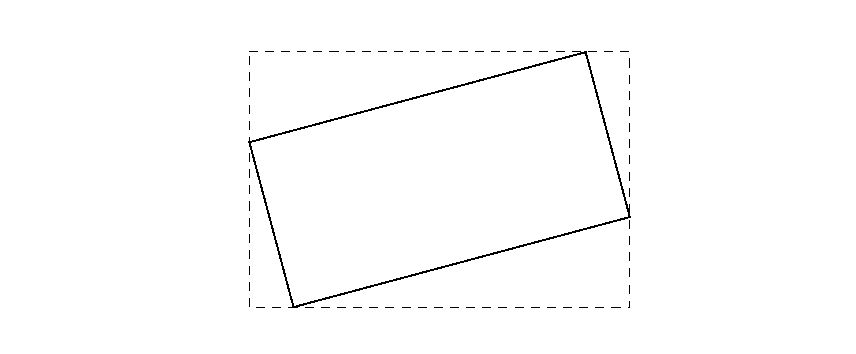
\includegraphics[width=\textwidth]{../img/kap3_rectangle_bounding}
	\caption{Čárkovaný \texttt{bounding rectangle} zobrazitelného prvku}
	\label{fig:bounding-rectangle}
\end{figure}

Rozhodli jsme se, že hit-testing bude na prvcích transformovaných rotací implementován tak, že se bod nejdříve porovná s~\texttt{bounding rectangle} a~v~případě úspěchu se provede přesné porovnání pomocí polorovin. V~případě prvků netransformovaných rotací stačí k~přesnému porovnání  použít pouze \texttt{bounding rectangle}. \texttt{Bounding rectangle} by bylo možné použít i~k~určení, zda se prvek nachází v~komponentě (\ref{kap3:view_element_bounding_check}) -- \texttt{bounding rectangle} by odpovídal červeným obdélníkům na plátně na obrázku \ref{fig:prvky_mimo_komponentu}. V~případě transformace rotací zabírá \texttt{bounding rectangle} o~něco více prostoru než je skutečná velikost prvku, ale jeho porovnání je rychlejší než přesné porovnání pomocí polorovin. Odhad, který používáme, v~nejhorších případech způsobí vykreslení velmi malého počtu prvků navíc.

\subsubsection*{Implementace zobrazitelných prvků}
\label{kap3:layout_cycle_view_element}
Implementaci zobrazitelných prvků bychom mohli reprezentovat rozhraním s~informacemi, které jsme si v~předchozích částech této podkapitoly uvedli. Toto rozhraní označíme jako \texttt{IViewElement}. Výhodou rozhraní by bylo, že~vývojář může implementovat vlastní cyklus rozmístění~z~\ref{spec:zobrazitelne_prvky2} podle konkrétního prvku metodami mimo rozhraní, odpovídající potřebám jeho implementace. Pokud \linebreak bychom například měli zobrazitelný prvek, který by představoval dopravní bod s~několika kolejemi, v~metodě umisťující prvek na plátno se nastaví, jestli má horizontální čáry jako koleje seskupit kvůli nedostatku prostoru na plátně do jedné čáry nebo je má vykreslit pro větší přehlednost vedle sebe.

Komplikací je, že pro implementaci rozhraní vývojář musí vypočítat přesné umístění prvků na~plátně \texttt{ContentCanvas}. V~případě práce se stromem prvků popisující obsah nákresného jízdního řádu podle \ref{spec:zobrazitelne_prvky1} by vývojář spíše preferoval možnost potomky prvku umístit v~rámci jeho souřadnic. Převod do souřadnic plátna \texttt{ContentCanvas} by se tak prováděl jen kvůli knihovně.

Další komplikací je aplikování strategií na prvky implementující toto rozhraní. Pokud bychom strom prvků přemístili nebo ho transformovali škálováním a~rotací, musí se změnit hodnoty pro výpočet \texttt{placement matrix} všech jeho prvků. Tento problém by musely řešit strategie úpravou hodnot rozhraní nebo by \texttt{IViewElement} mohlo obsahovat metody jako \texttt{Scale()} nebo \texttt{Rotate()}, které by strategie volaly a~úpravu stromu prvků by implementoval vývojář. V~předchozí části věnující se vlivu aplikování strategií na cyklus rozmístění jsme si ale uvedli, že by tyto operace měly implementaci prvku vývojářem ovlivnit co nejméně.

Informace rozhraní \texttt{IViewElement} se převádí na různé struktury jako \linebreak \texttt{placement matrix} nebo \texttt{bounding rectangle}. Všechny tyto převody by se odehrávaly během vykreslování, které ale nechceme zbytečně zpomalovat. Bylo by vhodnější, kdyby se už tyto struktury předpočítaly během cyklu rozmístění. Mohli bychom vytvořit základní implementaci zobrazitelných prvků, která implementuje nějaký obecný cyklus rozmístění, předpočítá tyto hodnoty a~umožní prvky umístit i~v~souřadnicích plátna rodičovského prvku.

Jelikož jsme určili, že by bylo vhodné, aby cyklus rozmístění produkoval další informace nebo struktury používané knihovnou, rozhodli jsme se, že jejich správné vytvoření zajistíme v~obecné implementaci, kterou dále budeme hledat. Vývojář bude v~potomcích základní implementace pouze přidávat konkrétní vlastnosti prvku -- vykreslení, určení požadované velikosti a~rozmístění obsahu na základě přiřazení konečné velikosti. Vývojáři tak obdrží hotovou implementaci, která bude vytvářet části důležité pro funkcionalitu knihovny.

\subsubsection*{Obecná implementace cyklu rozmístění zobrazitelných prvků}
Obecný cyklus rozmístění prvků musí být dostatečně konfigurovatelný pro různé scénáře. Podle \ref{spec:zobrazitelne_prvky2} například chceme změřit velikost prvku a~na základě této velikosti mu přiřadit jeho konečnou velikost. Konečná velikost prvku bude určovat velikost plátna pro vykreslení, ale i~hit-testovanou oblast nebo \texttt{bounding rectangle}. S~konečnou velikostí také budou pracovat strategie. Pokud by prvek tuto velikost přesáhl, nástroje by s~prvkem nemohly správně pracovat. Protože vytváříme nějakou obecnou implementaci pro knihovnu, chceme, aby špatné nastavení cyklu rozmístění bylo nějak deterministicky vyřešeno. Jelikož s~konečnou velikostí prvku pracuje mnoho částí knihovny, rozhodli jsme se, že pokud velikost prvku přesáhne přidělenou velikost, nebude rozmístěn. Problém s~rozmístěním se tak projeví hned a~ne při práci knihovny s~prvkem. Nechceme vyhovazovat výjimky, protože vytváříme obecnou implementaci a~některé aplikace pouze příliš velký prvek v~některých konfiguracích komponenty nezobrazí. Vývojáři umožníme ale implementaci rozšířit a~chybové stavy řešit i~jiným způsobem.

Podobný problém, na který jsme narazili, řeší i~GUI frameworky. Ty vytváří základní implementaci cyklu rozmístění pro jejich prvky uživatelského rozhraní. Frameworky pak pomocí hierarchie tříd cyklus rozmístění dále rozšiřují konfigurací jeho základní implementace. Toto řešení je vhodné i~pro naší knihovnu. Nemuseli bychom tak vymýšlet nové řešení, ale mohli bychom nějaké převzít a~upravit ho. Rozhodli jsme se proto použít nějakou existující implementaci a~přizpůsobit ji navíc požadavkům naší knihovny. Implementace se mezi různými frameworky zásadně neliší a~proto jsme se rozhodli vybrat k~implementaci cyklus rozmístění frameworku WPF, který se skládá z~\textit{measure} a~\textit{arrange} průchodů znázorněných na obrázku \ref{fig:arrange_WPF}:

\begin{figure}[!bht]
	\centering
	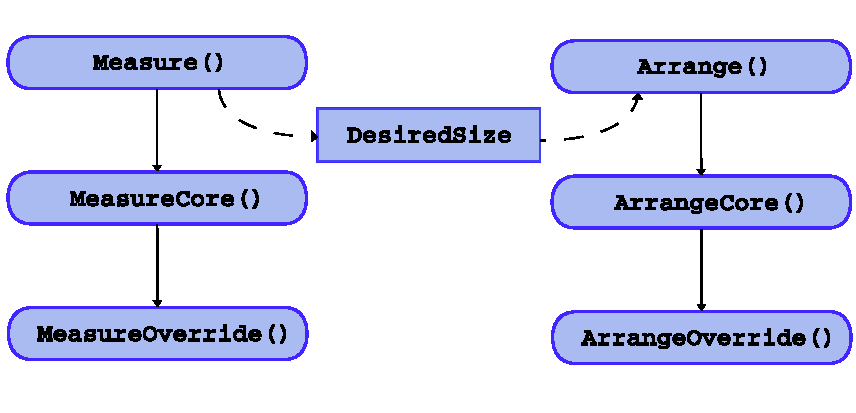
\includegraphics[width=\textwidth]{../img/kap3_wpf_element_layout_cycle_diagram}
	\caption{Schéma cyklu rozmístění pro prvek GUI frameworku WPF}
	\label{fig:arrange_WPF}
\end{figure}

Prvkům je možné nastavit vlastnosti jako \texttt{Margin}, \texttt{MinWidth}, \texttt{MaxWidth}, \linebreak \texttt{MinHeight}, \texttt{MaxHeight}. V~measure průchodu začínající metodou \texttt{Measure()} \linebreak nejdříve zjistíme velikost prvku. Velikost je v~rámci hierarchie volání získána nejdříve z~metody \texttt{MeasureOverride()}, kterou přetěžuje vývojář pro konkrétní implementaci prvku. Tato velikost je předána \texttt{MeasureCore()}, která v~základní implementaci ověřuje správnost vrácené hodnoty například vůči nastavení \linebreak \texttt{MaxWidth}, \texttt{MinWidth} a~případně ji upravuje. Vývojář může metodu přetížit za podobným účelem. Ověřená hodnota je předána \texttt{Measure()}, která ji přiřadí do vlastnosti \texttt{DesiredSize}. V~arrange průchodu je metodě \texttt{Arrange()} předána konečná velikost prvku. Metody \texttt{ArrangeOverride()} a~\texttt{ArrangeCore()} se chovají podobným způsobem jako jejich ekvivalenty v~measure průchodu. Cyklus rozmístění WPF vytváří mezi prvky explicitní vztahy, aby například invalidování potomka mohlo notifikovat o~změně rodiče, který by mohl změnu velikosti potomka vyřešit v~jemu přiřazené velikosti, případně by se notifikace šířila do jeho rodiče. Jelikož k~těmto situacím docházet při práci se zobrazitelnými prvky nebude, pro jednoduchost jsme se rozhodli explicitní vazby mezi prvky nevytvářet. Na potomky se volá pouze z~rodičovských prvků \texttt{Arrange()} a~\texttt{Measure()}.

\subsubsection*{Výpočet struktur používaných knihovnou v~cyklu rozmístění}
\label{kap3:upravy_zobrazitelnych_prvku_strategiemi}
Určili jsme, že v~základní implementaci cyklu rozmístění spočítáme hodnoty jako \texttt{placement matrix} nebo \texttt{bounding rectangle}. Navíc podle \ref{spec:req:strategie2} chceme, aby zobrazení prvků bylo možné upravovat rotací a~škálováním a~prvek přerozmístit. Všechny tyto úpravy je možné zahrnout do \texttt{placement matrix}. Při vykonávání těchto modifikací prvku chceme, aby byly aplikovány na všechny jeho potomky.

Jelikož se výpočet těchto hodnot bude aplikovat i~pomocí metod, kterými strategie prvek transformují a~je celkem náročné ho implementovat, chtěli bychom najít nějakou jednu metodu, v~které by se výpočet provedl. Pokud se podíváme, jak transformace souvisí s~cyklem rozmístění, strategie nejdříve musí zjistit velikost prvku, přiřadit mu konečnou velikost a~pak ho případně transformovat rotací nebo škálováním. Metoda \texttt{Arrange()}, která by prvku přiřadila konečnou velikost, by mohla získat v~rámci jejího volání \texttt{placement matrix}. Konfigurace \texttt{placement matrix} by pak mohly být následující:

\begin{enumerate}
	\item	Aplikováním \texttt{placement matrix} rodičovského prvku můžeme prvek \newline\texttt{Arrange()} umístit v~souřadnicích rodičovského prvku
	\item	Aplikováním \texttt{placement matrix} jako identity můžeme prvek \texttt{Arrange()} umístit v~souřadnicích \texttt{ContentCanvas}
	\item	Aplikováním rotace nebo škálování na \texttt{placement matrix} můžeme vytvářet transformace rotace a~škálování strategiemi
\end{enumerate}
 
Měli bychom tedy nějakou interní metodu \texttt{ArrangeInternal()}, která by přijímala různé \texttt{placement matrix}. Vývojáři by volali na zobrazitelném prvku \linebreak \texttt{Arrange()}, \texttt{Scale()}, \texttt{Rotate()} a~\texttt{Reposition()}. Tyto metody upraví \texttt{placement matrix} a~předají jí \texttt{ArrangeInternal()} metodě. Pokud se zavolá \linebreak v~\texttt{ArrangeOverride()} na potomka \texttt{Arrange()}, předá se mu upravená \texttt{placement matrix} a~stejný výpočet probíhá znovu v~potomku. Pomocí \texttt{placement matrix} se pak vypočítá \texttt{bounding rectangle} i~ostatní hodnoty související s~transformací. Ačkoliv cyklus rozmístění tak probíhá pro každou tuto operaci znovu, rozhodli jsme se tento přístup použít, protože neduplikuje kód a~aplikování operace znovu nepředstavuje velké výkonnostní omezení, jelikož transformace strategiemi neprobíhají na větších stromech prvků a~vyskytují se v~cyklu rozmístění, ke kterému při běhu aplikace nedochází často.

\newpage
\subsection{Kreslení po vrstvách}
\label{kap3:drawing_layers}
Podle podkapitoly \ref{kap2:drawing_layers} chceme umožnit obsah vykreslovat ve vrstvách. Ve zmíněné podkapitole jsme uvedli příklad, kdy chceme do nové vrstvy v~popředí vynést vybraný vlak z~vrstvy vykreslující všechny vlaky. Zásadní problém, kterému se budeme snažit předejít, je vykreslení stejného obsahu ve více vrstvách opakovaně -- vybraný vlak by se vykreslil v~nové i~původní vrstvě. Všechny vlaky se nachází v~nějakém seznamu a~v~původní vrstvě se vykreslí následovně:

\begin{csharpcode}
foreach(var train in Trains) {
	drawingCanvas.Draw(train);
}
\end{csharpcode}

Mohli bychom vybraný vlak umisťovaný do nové vrstvy z~\texttt{Trains} odebrat. Tímto ale zasahujeme do modelu aplikace, při operaci, která svým významem model nemění -- vybraný vlak se pouze přenáší do popředí. Další možností by bylo vytvořit nový seznam, který obsahuje prvky nacházejí se ve vrstvě nebo každému zobrazovanému vlaku přidat informaci, zda je ho možné ve vrstvě vykreslit. Zásadním problémem obou těchto řešení je fakt, že zasahují do implementace obsahu v~původní vrstvě:

\begin{csharpcode}
foreach(var train in Trains) {
	if (currentLayer.Contains(train)) {
		drawingCanvas.Draw(train);	
	}	
}
\end{csharpcode}

Problém můžeme řešit na úrovni knihovny tak, aby tato implementace nebyla změněna. Prvky jako vlak by implementovaly rozhraní \texttt{IVisual}, které bude nést informaci o~přidělené vrstvě prvku. \texttt{DrawingCanvas} bude vědět, jakou vrstvu vykresluje. Pokud budeme chtít \texttt{IVisual} na plátno vykreslit, nejdříve se provede porovnání vrstev a~pokud jsou stejné, prvek se vykreslí. Jediná nevýhoda je, že se vrstva musí přenastavit všem prvkům stromu reprezentující vybraný vlak, aby se po porovnání vykreslily.

Jelikož jsme v~požadavku \ref{spec:zobrazitelne_prvky1} určili, že obsah nákresného jízdního řádu bude systematicky popsatelný různými prvky, rozhodli jsme se, že prvky budou implementovat rozhraní jako \texttt{IVisual} a~\texttt{DrawingCanvas} ověří jejich vykreslení. \texttt{IVisual} bude implementováno v~nějaké základní třídě všech vykreslitelných prvků, která je předkem \texttt{ViewElement}. V~knihovně tak vytváříme mechanismus, který vývojář může používat a~nevytvářet vlastní řešení. Zmíněnou nevýhodu v~další části odstraníme a~ještě řešení vylepšíme.

\pagebreak
\subsubsection*{Konfigurace vrstev}
V~dosavadní představě si v rozhraní \texttt{IVisual} uchováváme pouze vrstvu, \linebreak v~které se prvek nachází. Když vývojář změní prvku vrstvu, musí si pamatovat, v~jaké předchozí vrstvě se prvek nacházel. Proces přemisťování prvků mezi vrstvami probíhá tak, že vývojář vrstvu změní a~pak ji zase nahradí původní. V~příkladu prvků vlaku vyneseného do popředí se jeho prvky nejdříve při inicializaci obsahu přiřadí do vrstvy všech vlaků a~při výběru vlaku se přenesou do vrstvy popředí. Pak se případně vrací do vrstvy původní. Proces přiřazování a~odebírání vrstev tak odpovídá práci se zásobníkem. Aby si vývojář nemusel pamatovat, v~jaké původní vrstvě se prvek nacházel, tento zásobník každému z~prvků přidáme.

Nevýhodou současného řešení je potřeba nastavovat vrstvu všem prvkům, které bychom chtěli vykreslit. Tuto nevýhodu bychom mohli na základě následujícího pozorování odstranit. Předpokládejme, že v~počátečním stavu aplikace problém, kdy by se jeden prvek vykreslil ve více vrstvách zároveň, nenastává. Chtěli bychom nalézt řešení, jak nastavování vrstev v~počátečním stavu přeskočit. Vytvoříme vrstvu, kterou nazveme jako \texttt{default layer}. Pokud ji má prvek nastavenou, kontrola vrstvy se před vykreslením nevykoná. Jelikož pracujeme se zásobníkem, bude tato vrstva umístěna na spodku zásobníku, jako počáteční stav. Pokud použijeme příklad s~vybraným vlakem, při jeho přesunu do nové vrstvy bychom už vrstvu změnili všem jeho prvkům.

\subsection{Implementace hit-testingu}
\label{kap3:hit_test_tree}
V~části \ref{kap3:element_hit_test} jsme určili, jak probíhá hit-testování na každém zobrazitelném prvku. Nyní si vysvětlíme, jak podle požadavku \ref{spec:req:hit-test2} implementujeme průchod zobrazitelných prvků obsahu nákresného jízdního řádu a~získáme z~něj ty, které v~hit-testování uspěly. Tyto prvky bude chtít vývojář získat podle pořadí jejich vykreslení, s~tím, že většinou bude pracovat s~prvkem, který je vykreslován v~popředí a~překrývá tak ostatní prvky, které v~hit-testu také uspěly. 

Průchod prvků by mohl implementovat sám vývojář. Postupně by procházel všechny prvky, tvořící dohromady stromovou strukturu. V~některých prvcích stromu by ale mohl narazit na problém. V~příkladu uvedeném v~\ref{kap3:drawing_layers} máme zobrazitelný prvek vykreslující všechny vlaky v~seznamu \texttt{Trains}. Vývojář by tento seznam prošel a~každý prvek vlaku ověřil v~hit-testu. Podle \ref{kap3:drawing_layers} se ale vlaky můžou nacházet v~různých vrstvách, čili by sekvenční průchod seznamu případně neposkytl správné pořadí vykreslení a~při průchodu prvků ve více vrstvách by se konkrétní prvek mohl vyskytnout v~úspěšně otestovaných prvcích vícekrát.

Průchod stromu prvků jsme se proto rozhodli implementovat v~knihovně. Otestování celého obsahu odpovídá průchodu stromem, kdy otestujeme obsah rozdělený do vrstev, vykreslovaných podle jejich pořadí. Každá vrstva bude obsahovat prvek, který bude kořenem jejího obsahu. K~rozhraní \texttt{IVisual} z~\ref{kap3:drawing_layers} bychom přidali metodu \texttt{HitTest()}, hit-testující vizuální prvek vůči nějakému bodu a~metodou poskytující potomky k~hit-testování \texttt{ProvideChildrenToHitTest()}. Z~této metody se pak vyberou jen ty prvky, které se nachází ve stejné vrstvě jako rodičovský prvek. Musíme ještě určit pořadí, v~kterém bude knihovna poskytovat úspěšně otestované prvky. Metodu \texttt{ProvideChildrenToHitTest()} bychom chtěli nechat vývojáře implementovat tak, aby prvky poskytovala v~pořadí vykreslení:

\begin{csharpcode}
public void OnDraw(DrawingCanvas drawingCanvas) {
	foreach(var train in Trains) {
		drawingCanvas.Draw(train);	
	}
}

public IEnumerable<IVisual> ProvideChildrenToHitTest() {
	foreach(var train in Trains) {
		yield return;
	}
}
\end{csharpcode}

To ale znamená, že první poskytnutý prvek je ten, který se vykreslí na spodku. Vývojář by mohl projít seznam v~opačném pořadí, to ale představuje komplikaci v~implementaci rozhraní. Úspěšně otestované prvky bychom při průchodu stromem mohli uchovávat v~nějakém seznamu, odpovídající pořadí vykreslení. Jelikož úspěšně testovaných prvků je malé množství, rozhodli jsme se, že vývojář v~rozhraní poskytne prvky podle pořadí vykreslení. Průchod tedy bude implementován tak, že se postupně navštíví všechny vrstvy s~jejich obsahem podle pořadí vykreslení. Pokud chceme prvek, který překrývá ostatní, najdeme ho na konci tohoto seznamu. Proto bychom si místo seznamu mohli pamatovat jen jeden prvek, který se vykreslí jako poslední. Bylo by možné místo pevného seznamu použít jinou implementaci průchodu, kterou si nyní představíme.

Průchod stromu prvků pro hit-testování řeší i~uživatelská rozhraní. Například GUI framework WPF implementuje obecný průchod stromem, kdy se při navštívení prvku zavolá vývojářem dodaná metoda delegáta \texttt{HitTestFilterCallback}, v~které může vývojář podle prvku rozhodnout, jak má dále průchod stromem pokračovat. Průchodu stromem se dále předává metoda delegáta \linebreak \texttt{HitTestResultCallback}, která se volá, pokud byl prvek vůči hit-testingu \linebreak úspěšný. Také určí, jak při průchodu stromem pokračovat. V~základním nastavení je tato implementace lehká na konfiguraci -- v~\texttt{HitTestResultCallback} by se úspěšně testované prvky přidávaly do seznamu, který jsme chtěli v~původní implementaci použít.
Vývojář může průchod stromem urychlit, jelikož dodání implementace delegáta \texttt{HitTestFilterCallback} umožňuje přeskočit všechny prvky v~nějakém podstromu, u~kterých víme, že se s~nimi pracovat nebude. Jelikož implementace odpovídá našim potřebám a~můžeme převzít funkční kód doplněný o~potencionálně využitelná rozšíření, rozhodli jsme se ji použít.

\newpage
\subsection{Implementace strategií}
\label{kap3:implementace}
Pro splnění požadavku \ref{spec:zobrazitelne_prvky1} musíme najít nástroje, které umožní systematicky popsat proces implementace strategií. Rozhodli jsme se, že tento proces rozdělíme do částí, kde každá část má jednu zodpovědnost\footnote{Single responsibility principle~\cite{Martin:2003:ASD:515230}}. Tyto částí si nyní popíšeme a~zdůvodníme jejich používání.

\subsubsection*{Segmenty strategií}
Strategiím je potřeba vyhradit nějaký vodorovný pruh, do kterého můžou umístit zobrazitelné prvky. Tyto pruhy označíme jako \textit{segmenty}. Umístění i~výšku segmentu vývojář určí v~cyklu rozmístění před samotným aplikováním strategie, jelikož jsou segmenty součástí zobrazitelných prvků popisujících nákresný jízdní řád, jako třeba místa pro umisťování kót kolem horizontálních čar dopravních bodů. Nechceme, aby vývojář vytvářel ve svém modelu vlastní struktury, které by segmenty určovaly. Nemůžeme pak jejich konkrétní implementaci zapojit do nástrojů pracujících se strategiemi a~navíc představují další část pro vývojáře, kterou musí implementovat. Ke strategii pro rozmisťování kót do ostrých úhlů bychom potřebovali dva segmenty kolem dopravních bodů, jako na obrázku \ref{fig:segments_upper_lower}. Segmenty v~příkladu je možné rozlišit -- podle dopravního bodu a~dolního nebo horního umístění. Proto pro segment zavedeme identifikaci označovanou jako \texttt{SegmentType}, která umožní segmenty kategorizovat. Segmenty patřící pod jeden typ bude spravovat registr \texttt{SegmentRegistry}, který bude přijímat registrace segmentů a~poskytovat segmenty podle \texttt{SegmentType}, čehož můžou využít další nástroje pracující se strategiemi.

\begin{figure}[!bth]
	\centering
	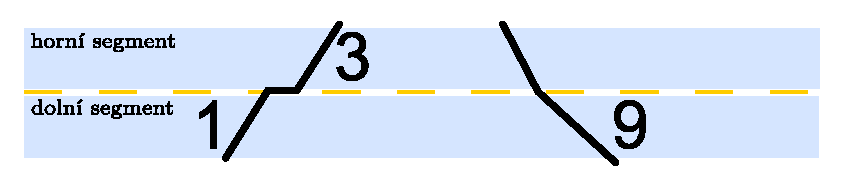
\includegraphics[width=\textwidth]{../img/kap3_segment_upper_lower}
	\caption{Horní a~dolní segment dopravního bodu pro umístění kót}
	\label{fig:segments_upper_lower}
\end{figure}

\subsubsection*{Zařazení zobrazitelných prvků do strategií}
\label{kap4:strategy_placement_type}
Když chce vývojář přidat do strategie zobrazitelný prvek, musí se zjistit, do jakého \texttt{SegmentType} prvek patří. Pokud by vývojář přidával prvek přímo do segmentu, musel by sám určit \texttt{SegmentType}. To ale může představovat problém. Uvažme případ, kdy chceme přidat odjezdovou kótu z~nějakého dopravního bodu, jako na obrázku \ref{fig:view_element_strategy_registration}. \texttt{SegmentType} je závislý na směru jízdy vlaku, čili vývojář musí sám složitě podle výpočtu zjistit, kam prvek podle směru patří. Vývojář by mohl při přidání prvku uvést jiný typ, přirozenější pro specifikaci umístění, označovaný jako \texttt{PlacementType}, který se na \texttt{SegmentType} převede. Vývojář by při přidání prvku uvedl informaci v~\texttt{PlacementType} 
\includegraphics[height=10.0pt]{../img/cas_osa_typ_1} se směrem (příjezd nebo odjezd). Bude pak existovat rozhraní \texttt{ITypeConverter}, které převede tuto informaci na \texttt{SegmentType} 
\includegraphics[height=10.0pt]{../img/cas_osa_typ_2} (lower, upper). Rozhodli jsme se tyto dva typy s~rozhraním pro převod zavést.

\begin{figure}[!bth]
	\centering
	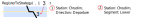
\includegraphics[width=\textwidth]{../img/kap3_view_element_segment_registration}
	\caption{Přidání kóty odjezdu do strategie}
	\label{fig:view_element_strategy_registration}
\end{figure}

\subsubsection*{Spravování zobrazitelných prvků v~strategiích}
Vývojář bude přidávat prvky do strategie pomocí nástroje \texttt{StrategyManager} uvedením \texttt{PlacementType}. \texttt{StrategyManager} 
zajišťuje přiřazení prvků do správných segmentů a~strategií. Vývojář tak nemusí přímo pracovat s~jejich konkrétními implementacemi. Existují situace, kdy je nutné invalidovat všechny přidané zobrazitelné prvky -- například, když se odstraňuje vlak nebo se jeho trasa zcela mění. Pro každý logický celek prvků, který má omezenou dobu existence (\textit{scope}), bude vytvořen nový \texttt{StrategyManager}, zajišťující odstranění prvků ze struktur strategií nebo segmentů -- zabraňujeme tak \textit{memory leakům}, kdy by tyto struktury držely jedinou referenci na prvek jinak již neexistující části obsahu, jelikož je vývojář zapomněl odebrat.

\subsubsection*{Dockery zobrazitelných prvků}
\textit{Docker} implementuje vhodné rozmístění zobrazitelných prvků. V~cyklu rozmístění obdrží od \texttt{StrategyManager} všechny přidané prvky a~umístí je do oblastí segmentů. Implementace dockeru může vypadat tak, že nejdříve prvek změří, přidělí mu požadovanou velikost přes \texttt{Arrange()} a~pak na něj podle \texttt{SegmentType} a~dalších parametrů aplikuje správnou metodu, která ho podle \ref{spec:req:strategie2} transformuje a~umístí. Docker je takto možné v~aplikaci vyměnit a~reimplementovat, jelikož přímo není propojený s~nástroji pro strategii.
\chapter{Vývojová dokumentace knihovny GTTG}
Ve Visual Studio 2017 \textit{solution} se nachází celý obsah práce, kde knihovna GTTG je jednou z~jeho částí.
Představíme si, jak je celý solution strukturovaný a~jaké jsou jeho další části. Solution jsme rozdělili
do tří složek:
\newline
\newline
\renewcommand\arraystretch{1.2}
\begin{tabular}{ m{0.1\textwidth} m{0.84\textwidth} }
\texttt{build} & Společná nastavení verzí balíčků používána v~projektech. Na soubory v~\texttt{build} typu \textit{*.props} obsahující verze balíčků se odkazují projekty v~\textit{.csproj} souborech.\\
\texttt{src} & Zdrojový kód v~solution\\ 
\texttt{test} & Unit testy pro zdrojový kód v~\texttt{src}
\end{tabular}
\newline
\newline
Solution je rozděleno do sedmi projektů uvedených na obrázku \ref{fig:kap4:solution_structure}, představující dvě části -- knihovnu GTTG, jejímuž popisu jsme se doposud věnovali, a~aplikaci SZDC, implementující práci s~grafikonem vlakovy využitím knihovny podle cíle \textbf{\ref{uvod:cil:aplikace}}. Popisu aplikace se budeme věnovat v~kapitole \ref{kap6:szdc_app}.

\begin{figure}[!hbt]
	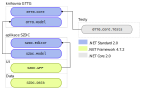
\includegraphics[width=\textwidth]{../img/kap4_solution_structure}
	\caption{Struktura projektů v~solution}
	\label{fig:kap4:solution_structure}
\end{figure}

Podle cíle~\textbf{\color{goalcolor}G2}\ref{uvod:cil:knihovna:dotnet_standard} jsme pro co největší přenositelnost knihovny GTTG všechny její projekty  implementovali vůči rozhraní .NET Standard 2.0. Jelikož podle cíle \textbf{\color{goalcolor}G2}\ref{uvod:cil:aplikace:vice_gui} chceme logiku aplikace SZDC zapojit do více uživatelských rozhraní, je také její editor \texttt{SZDC.Editor} a~model dat \texttt{SZDC.Model} implementován vůči rozhraní .NET Standard. Jako GUI framework aplikace \texttt{SZDC} jsme zvolili WPF, který je v~naší aplikaci spustitelný na běhovém prostředí .NET Framework 4.7.2. Nově je možné i WPF spustit na běhovém prostředí .NET Core 3. Výběru GUI frameworku a~běhového prostředí pro zvolené WPF se věnujeme v~kapitole \ref{kap6:szdc_gui_framework}.

\subsubsection*{Struktura knihovny GTTG}
Knihovna je rozdělena do dvou spolu souvisejících částí, jejichž schéma rozdělení se nachází na obrázku \ref{fig:kap4:gttg_lib_structure}.

\texttt{GTTG.Core} obsahuje nástroje umožňující uživatelskou interakci s~knihovnou a~její integraci do aplikací. Základem knihovny je \textit{engine} \texttt{GraphicalComponent} a~nástroj \texttt{DrawingManager} rozdělující kreslení do vrstev. Dále jsou v~projektu implementovány prvky umožňující systematicky popsat implementaci nákresných jízdních řádů, jako třeba \texttt{ViewElement} a~\texttt{Visual}. 
Projekt obsahuje nástroje pro práci s~těmito prvky, jako třeba \texttt{HitTestManager} a~nabízí rozhraní jako \linebreak\texttt{IStrategyDocker}, jehož implementací vytváří vývojář strategie umisťující prvky jako kóty do nákresného jízdního řádu.

\texttt{GTTG.Model} používá \texttt{GTTG.Core} k~vytvoření základního modelu nákresných jízdních řádů. Třídy jako \texttt{TrainView} jsou potomky základní třídy zobrazitelných prvků \texttt{ViewElement} a~představují vizualizaci datového modelu tříd jako \texttt{Train} nebo \texttt{Station}. Projekt tak rozděluje třídy na \textit{view model} a~\textit{model}. Dále jsou v~projektu implementována rozhraní knihovny \texttt{GTTG.Core} pro práci se zobrazitelnými prvky. Například \texttt{TracksStrategyDocker} jako implementace rozhraní \texttt{IStrategyDocker} z~\texttt{GTTG.Core} rozmisťuje kóty \includegraphics[height=10.0pt]{../img/cas_osa_typ_1} do ostrých úhlů průběhu jízdy vlaku \texttt{TrainView}.

\begin{figure}[!hbt]
	\centering
	\includegraphics[width=.85\textwidth]{../img/kap4_gttg-lib-structure}
	\caption{Části knihovny GTTG}
	\label{fig:kap4:gttg_lib_structure}
\end{figure}

\section{GTTG.Core}
\texttt{GTTG.Core} \textit{assembly} je rozdělena do několika oblastí jmenných prostorů:

\begin{tabular}{ m{0.15\textwidth} m{0.70\textwidth} }
\texttt{Base} & Hierarchie tříd implementující zobrazitelné prvky \\
\texttt{Component} & Třídy pro práci s~grafickou komponentou \\ 
\texttt{Drawing} & Nástroje pro kreslení \\
\texttt{Extensions} & Knihovní a~SkiaSharp \textit{extension} metody \\
\texttt{HitTest} & Nástroje pro hit-testování obsahu \\
\texttt{Strategies} & Nástroje pro práci se strategiemi \\
\texttt{Time} & Třídy pro reprezentaci časových intervalů \\
\texttt{Utils} & Matematické funkce pro implementaci strategií
\end{tabular}
\newline
\newline
V~následujících částech si tyto jmenné prostory popíšeme.

\subsection{Grafická komponenta}
\label{kap4:graphical_component}
Základem knihovny GTTG je třída \texttt{GraphicalComponent} představující \textit{engine}, který umožňuje vytvářet pohled na nákresný jízdní řád podle interakcí uživatele s~aplikací nebo jiných nastavení, jako na obrázku \ref{fig:kap4:gttg-core-graphical-component}. Poskytuje modifikace jako translace a~škálování pohledu v~rámci ohraničení nákresného jízdního řádu. Na základě nastavení pohledu pak vzniká stav komponenty, s~kterým pracují ostatní části knihovny. Například vykreslení nákresného jízdního řádu je nastaveno maticí \texttt{ContentMatrix},  kterou podle \ref{fig:analyza_impl:platno} třída modifikacemi upravuje.

\begin{figure}[!hbt]
	\includegraphics[width=\textwidth]{../img/kap4_gttg-core-graphical-compont}
	\caption{\textit{Engine} \texttt{GraphicalComponent}}
	\label{fig:kap4:gttg-core-graphical-component}
\end{figure}

Obrázek \ref{fig:kap4:gttg-core-component_structure_diagram} obsahuje schéma tříd jmenného prostoru \texttt{GTTG.Core.Component} související s~implementací grafické komponenty, jehož součásti si nyní blíže představíme:

\begin{figure}[!hbt]
	\includegraphics[width=\textwidth]{../img/kap4_gttg-core-component_structure_diagram}
	\caption{Schéma tříd a~rozhraní implementujících grafickou komponentu}
	\label{fig:kap4:gttg-core-component_structure_diagram}
\end{figure}

\newpage
Stav komponenty \ref{spec:req:state} je představován vlastnostmi, které jsou mimo třídu pouze pro čtení. Abychom mohli stav v~komponentě poskytnou dalším částem knihovny nebo implementacím bez přístupu k~modifikacím komponenty, \linebreak\texttt{GraphicalComponent} implementuje rozhraní \texttt{IViewProvider}. Rozhraní poskytuje i~převody mezi body komponenty a~časovými údaji, které jsou využívány nástroji knihovny (průběh jízdy vlaku se vykreslí převodem jeho časových údajů do souřadnic) nebo naopak aplikační logikou pracující s~knihovnou, která chce souřadnice kurzoru myši v~komponentě převést na časový údaj zobrazený v~aplikaci.

Komponenta pracuje s~třídou \texttt{ViewModifier} určenou pro vykonávání složitějších matematických modifikací stavu komponenty. Implementace modifikací v~\texttt{GraphicalComponent} upraví parametry a~předá je odpovídající modifikaci ve \texttt{ViewModifier}. V~případě úspěšné modifikace je pak upraven celý stav komponenty. Každá modifikace vrací podle \ref{kap3:modifikace_komponenty} výčtový typ nesoucí informace
o~jejím výsledku.

\subsubsection*{Práce s~časovými údaji}
Knihovna obsahuje strukturu \texttt{DateTimeInterval} představující časové intervaly \texttt{DateTime} hodnot. \texttt{GraphicalComponent} tuto strukturu používá k~reprezentaci časových intervalů v~komponentě popsaných v~\ref{kap2:time_intervals}. Třídou \texttt{DateTimeContext}, která tyto intervaly slučuje a~zajišťuje jejich validitu, se můžou komponentě v~rámci jejího stavu přenastavit časové intervaly. Pohled na nákresný jízdní řád je pak možné modifikovat i~pomocí časových intervalů jako v~situacích zmíněných v~\ref{kap2:modifikace_cas_intervaly}.

\subsection{Vykreslování}
Obsah knihovny je vykreslován ve vrstvách, které jsou reprezentovány rozhraním \texttt{IDrawingLayer} s~metodou \texttt{Draw()} k~vykreslení vrstvy. Podle schématu \ref{fig:kap4:drawing_layers_diagram} abstraktní třída \texttt{DrawingLayer} implementuje toto rozhraní a~je předkem tří abstraktních typů vrstev:

\hskip-1.0cm
\begin{tabular}{ m{0.33\textwidth} m{0.63\textwidth} }
\texttt{ContentDrawingLayer} & Typ vrstvy, které je k~vykreslení poskytnuto plátno pro celý obsah nákresného jízdního řádu podle \ref{spec:req:canvas1}. \\
\texttt{ViewDrawingLayer} & Typ vrstvy, které je k~vykreslení poskytnuto plátno komponenty podle \ref{spec:req:canvas2}. \\ 
\texttt{DefaultDrawingLayer} & \textit{Singleton} reprezentující vrstvu, která je při kontrole vrstvy v~\ref{kap3:drawing_layers} vždy validní.
\end{tabular}

\begin{figure}[!hbt]
	\centering
	\includegraphics[width=\textwidth]{../img/kap4_gttg-core_drawing_layers1}
	\caption{Schéma tříd a~rozhraní představující vrstvy}
	\label{fig:kap4:drawing_layers_diagram}
\end{figure}

\subsubsection*{Správa kreslících vrstev}
Třída \texttt{DrawingManager} vykresluje vrstvy podle pořadí definovaného vývojářem. Instance vrstev jsou přidávány s~určením jejich pořadí pomocí metod \texttt{AddOnCurrentTop()}, \texttt{AddOnCurrentBottom()}, \texttt{Insert()}. Instanci vrstvy je \linebreak možné odstranit pomocí \texttt{RemoveDrawingLayer()}. Jelikož existují vrstvy, které se neodstraňují a~jejich pořadí je během běhu aplikace neměnné, konstruktoru \texttt{DrawingManager} se předává implementace rozhraní \texttt{IRegisteredLayersOrder}, které obsahuje pořadí typů (z~\texttt{typeof()}) vrstev, které označíme jako \textit{registrované}. Takovou vrstvou může být vrstva svislých čar reprezentující časové údaje nebo vrstva s~dopravními body. Metoda \texttt{ReplaceRegisteredDrawingLayer()} umístí instanci registrované vrstvy podle jejího  typu v~pořadí určeným~rozhraním.

\subsubsection*{Kreslící plátno}
Knihovna na plátno \texttt{SKCanvas}, které ji poskytne vývojář, vytváří různé pohledy. Tyto pohledy budeme reprezentovat plátnem \texttt{DrawingCanvas}. Vhodným nastavením \texttt{transformation matrix} na \texttt{SKCanvas} může \texttt{DrawingCanvas} představovat plátno pro vykreslování zobrazitelných prvků z~\ref{kap3:vykresleni_zobrazitelnych_prvku} i~celého obsahu plátna \texttt{ContentCanvas} z~\ref{fig:analyza_impl:platno}. Plátno nabízí kreslící příkazy \texttt{SKCanvas} a~příkazy pro vykreslení prvků knihovny. Plátno obsahuje vlastnosti o~své velikosti \texttt{Width}, \texttt{Height}. Vlastnost \texttt{DrawingLayer} udává, v~jaké vrstvě bylo plátno vytvořeno.

\subsubsection*{Proces vykreslování vrstev}
\textit{Entry pointem} pro vykreslení obsahu knihovny je metoda \texttt{Draw(SKSurface surface)} ve třídě \texttt{DrawingManager}. Vrstvy se vykreslí v~sestaveném pořadí tak, že se pro každou vrstvu zavolá metoda \texttt{CreateCanvas()} factory rozhraní \linebreak\texttt{ICanvasFactory}, která poskytnutím \texttt{IDrawingLayer} a~\texttt{SKCanvas} vytvoří pro vrstvu konfigurovaný \texttt{DrawingCanvas}. Vrstvám \texttt{ContentDrawingLayer} \linebreak a~\texttt{ViewDrawingLayer} poskytuje knihovna implementaci rozhraní \texttt{CanvasFactory}.

\begin{figure}[!hbt]
	\includegraphics[width=\textwidth]{../img/kap4_gttg-core_drawing_canvases}
	\caption{Modře ohraničený \texttt{ContentDrawingCanvas} a~červeně ohraničený \texttt{ViewDrawingCanvas}}
	\label{fig:kap4:gttg-core-base_canvases}
\end{figure}

\newpage
\subsection{Zobrazitelné prvky}
Jmenný prostor \texttt{GTTG.Core.Base} obsahuje hierarchii tříd uvedenou na obrázku \ref{fig:kap4:gttg-core-base_class_hierarchy}, z~níž vzniká třída \texttt{ViewElement} představující zobrazitelné prvky určené k~systematickému popisu nákresného jízdního řádu podle \ref{kap2:view_elements}.

\begin{figure}[!hbt]
	\includegraphics[width=\textwidth]{../img/kap4_gttg-core-base_class_hierarchy}
	\caption{Hierarchie tříd tvořící zobrazitelné prvky}
	\label{fig:kap4:gttg-core-base_class_hierarchy}
\end{figure}

\subsubsection*{ObservableObject}
\label{kap4:observable_object}
Na začátku hierarchie tříd se nachází abstraktní třída \texttt{ObservableObject} implementující rozhraní \texttt{INotifyPropertyChanged}, které slouží k~notifikacím o~změnách vlastností v~třídě pomocí eventu \texttt{PropertyChanged}. Tuto základní třídu mohou využít vývojáři k~vytvoření \textit{data bindingu} z~uživatelských rozhraní na aplikační logiku a~její model. Pokud bychom měli například model vlaku \texttt{Train} obsahující plán jízdy \texttt{Schedule}, aplikace by \texttt{Schedule} navíc zobrazovala v~jiné komponentě uživatelského rozhraní jako textová data. V~případě, kdy by se \texttt{Schedule} změnila, notifikaci o~změně obdrží jiná komponenta v~aplikaci a~zároveň i~\texttt{TrainView}, které může upravit svou vizualizaci dat. Z~této třídy dědí \texttt{GraphicalComponent}, která tak umožňuje vývojářům získávat notifikace o~změně \texttt{DateTimeContext}. 

Třída implementuje mechanismus pro bezpečné a~lehké používání notifikací na \textit{setterech} vlastností, který jsme převzali z~projektu \texttt{Core2D}~\cite{Core2D} z~třídy \linebreak\texttt{ObservableObject}. Následující fragment kódu ukazuje přiřazení nové hodnoty do vlastnosti s~notifikováním pomocí \texttt{Update()} metody. Update by se jinak musel provádět pomocí \textit{invoke} eventu \texttt{PropertyChanged} poskytnutím jména vlastnosti.

\begin{csharpcode}
public class GraphicalComponent {
	
	public DateTimeContext DateTimeContext  {
		get => _dateTimeContext;
		protected set => Update(ref _dateTimeContext, value);	
	}
	
\end{csharpcode}
\newpage
\subsubsection*{Visual}
Abstraktní třída \texttt{Visual} představuje prvky, které popisují nákresný jízdní řád a~je možné je vykreslit na \texttt{DrawingCanvas}, ale narozdíl od zobrazitelných prvků se nerozmisťují. Příkladem může být prvek \texttt{TrafficView}, který sdružuje a~vykresluje na plátno \texttt{ContentDrawingCanvas} všechny vlaky \texttt{TrainView}. \texttt{Visual} obsahuje podle \ref{kap3:drawing_layers} zásobník vrstev \texttt{IDrawingLayer} s~neměnným spodkem obsahující singleton \texttt{DefaultDrawingLayer}. Vlastnost \texttt{CurrentDrawingLayer} odpovídá vrchu zásobníku. Vykreslení probíhá tak, že se virtuální metodě \texttt{Draw()} předá \texttt{DrawingCanvas} a~nejdříve se ověří možnost prvek vykreslit pomocí \linebreak \texttt{IsInDrawingLayer()} porovnáním \texttt{CurrentDrawingLayer} a~\texttt{DrawingLayer} \linebreak plátna. Po ověření se zavolá virtuální \texttt{protected OnDraw()} k~vykreslení implementace prvku.

Vyvojáři implementují \texttt{protected} \texttt{ProvideVisuals()}, která dodává prvky v~pořadí vykreslení. Metoda je volána \texttt{ProvideVisualsInSameLayer()} poskytující pouze z~těchto prvků ty, které se nachází ve stejné vrstvě jako prvek, na kterém se metoda volá. Tyto metody se používají při hit-testování a~nastavování vrstev potomkům.

Pro případy, kdy existující prvek (například model jako potomek jiné třídy) nemůže již od \texttt{Visual} dědit a~přesto chce kreslit na plátno, použije rozhraní \texttt{IVisual}, s~kterým pak pracuje i~kód knihovny jako s~reprezentací \texttt{Visual}. Rozhraní se používá i~pro \textit{mockování} v~unit testech.

\subsubsection*{ViewElement}
Abstraktní třída \texttt{ViewElement} představuje základní implementaci zobrazitelných prvků z~podkapitoly \ref{kap3:zobrazitelne_prvky}, které je možné umístit a~určit jim velikost. Pro implementaci cyklu rozmístění \texttt{ViewElement} jsme použili cyklus rozmístění prvků uživatelského rozhraní GUI frameworku WPF. Implementace jeho metod na schématu \ref{fig:arrange_WPF_kap4} odpovídá zdrojovému kódu metod z~WPF, který byl ale upraven, aby mohl vytvářet během cyklu rozmístění i~struktury, s~kterými pracuje knihovna.

\begin{figure}[!bht]
	\centering
	\includegraphics[width=\textwidth]{../img/kap3_wpf_element_layout_cycle_diagram}
	\caption{Schéma cyklu rozmístění pro prvek GUI frameworku WPF}
	\label{fig:arrange_WPF_kap4}
\end{figure}

\newpage
Metody \texttt{Arrange()} a~\texttt{Measure()} zajišťují správné používání virtuálních metod typu \texttt{Core}, které volají. Ty slouží k~určení obecné implementace prvků, která se používá v~rámci nějaké aplikace. V~základní implementaci upravují vrácené hodnoty z~\texttt{Override} metod. Ty jsou určeny ke změření a~rozmístění konkrétního prvku. V~rámci volání metody \texttt{Arrange()} se podle \ref{kap3:zobrazitelne_prvky} vytváří struktury, s~kterými knihovna pracuje:

\hskip-1.0cm\renewcommand\arraystretch{1.5}
\begin{tabular}{ m{0.3\textwidth} m{0.65\textwidth} }
\texttt{BoundingRectangle} & Obdélník k~určení, zda se prvek nachází v~komponentě podle \ref{fig:analyza_impl:platno}. \\
\texttt{PlacementMatrix} & Matice \texttt{placement matrix} pro vytvoření \texttt{transform matrix} plátna \texttt{DrawingCanvas} z~\ref{kap3:vykresleni_zobrazitelnych_prvku}. \\
\texttt{Clip} & Oblast ořezu vykreslení z~\ref{kap3:skia_intro_transformations} pokrývající prvek, která se může aplikovat pomocí vlastnosti \texttt{HasClipEnabled}. \\ 
\end{tabular}
\newline
\newline
Přetíženou metodou \texttt{Arrange()} se prvek umístí na plátno \texttt{ContentCanvas} -- přímo v~jeho souřadnicích nebo v~souřadnicích již umístěného prvku, který se uvede jako parametr \texttt{Arrange()} metody. To je užitečné v~případě, kdy \linebreak v~\texttt{ArrangeOverride()} rodičovského prvku získáme konečnou velikost rodiče \linebreak a~musíme v~rámci této velikosti rozmístit jeho potomky \texttt{Arrange()} metodou. Zároveň \texttt{ViewElement} implementuje metody \texttt{Reposition()}, \texttt{Scale()} a~\texttt{Rotate()}, které jsou používány strategiemi. Transformované zobrazení prvku je popsáno vlastnostmi, které jsou zobrazeny na obrázku \ref{fig:kap4:gttg-view-element-properties}. Vlastnosti s~prefixem \texttt{Content} odpovídají transformované velikosti a~umístění. Vlastnost umístění jako \linebreak\texttt{ContentRightTop} odpovídá umístění netransformovaného horního pravého vrcholu po aplikování transformace.

\begin{figure}[!hbt]
	\centering
	\includegraphics[width=\textwidth]{../img/kap4_gtttg-core-element-transform-properties}
	\caption{Popis vlastností \texttt{ViewElement}}
	\label{fig:kap4:gttg-view-element-properties}
\end{figure}

\subsection{Průchod stromu prvků pro hit-testování}
Průchod stromu prvků \texttt{Visual} hit-testováním popsaný v~\ref{kap3:hit_test_tree} je implementován třídou \texttt{HitTestManager} v~přetížených metodách \texttt{HitTest()}. Průchod stromem je implementován podle implementace GUI frameworku WPF -- vývojář poskytuje metody delegátů \texttt{HitTestResultCallback} a~
\texttt{HitTestFilterCallback} pro řízení průchodu stromem a~získání úspěšně otestovaných prvků, více popsané v~\ref{kap3:hit_test_tree}. Vývojáři jsou dostupná přetížení metody \texttt{HitTest()}, která se svým chováním liší. Prvky jsou pokaždé poskytovány v~pořadí jejich vykreslení. První přetížení s~parametry dvou zmíněných delegátů prochází celý obsah nákresného jízdního řádu po vrstvách, kdy z~každého prvku \texttt{Visual} navštíví potomky pouze ve stejné vrstvě pomocí \texttt{ProvideVisualsInSameLayer()}. \texttt{HitTestManager} obdrží pořadí vrstev v~konstruktoru z~\texttt{DrawingManager}.
Druhému přetížení se dodává navíc prvek \texttt{Visual} a~při průchodu se získávají potomci z~\texttt{ProvideVisuals()}, poskytující prvky i~v~jiných vrstvách. Seznam prvků \texttt{Visual}, které uspěly v~hit-testu, je pak možné seřadit pomocí \textit{extension} metody \texttt{OrderByLayers()} podle pořadí vrstev. Druhé přetížení je určeno pro případy, kdy vývojář testuje obsah umístěný původně v~jedné vrstvě a~je možné, že jeho část je nyní součástí jiné vrstvy, například při testování seznamu vlaků, kdy vlaky můžou být rozděleny do více vrstev podle jejich zařazení a~nechceme procházet celý vykreslovaný obsah. Předpokládá se, že při průchodu podstromu poskytnutého prvku se navštíví všechny prvky pouze jednou.

\subsection{Nástroje pro strategie}
V~této části si představíme implementaci nástrojů pro práci se strategiemi, které jsme si popsali v~\ref{kap2:strategies_introduction}. Na obrázku \ref{fig:kap4:gttg-strategy_tools_schema} se nachází závislosti mezi těmito nástroji. Instance třídy \texttt{Segment} představují pruhy, jejichž umístěním a~velikostí vývojář určuje místa, do kterých mají strategie rozmisťovat prvky. Přidání prvků do strategie probíhá ve třídě \texttt{StrategyManager}, která podle informací dodaných při přidávání prvku daný prvek zařadí do vhodného segmentu. Během cyklu rozmístění pak \texttt{IStrategyDocker} představující implementaci strategie obdrží všechny přidané prvky a~umístí je do segmentů podle pravidel strategie.

\begin{figure}[!hbt]
	\centering	
	\includegraphics[width=0.8\textwidth]{../img/kap4_gtttg-core-strategies-tools}
	\caption{Schéma nástrojů pro práci se strategiemi}
	\label{fig:kap4:gttg-strategy_tools_schema}
\end{figure}

\subsubsection*{Segmenty}
\label{kap4:segments}
Třída \texttt{Segment} představuje podle \ref{kap3:implementace} ohraničený horizontální pruh, kterému se určuje výška. Podle výšky segmentu se do něj strategiemi rozmisťují prvky. Pokud je segment pro prvek příliš krátký, může strategie podle \ref{kap2:strategies_introduction} prvek zmenšit škálováním. Výška segmentu se určuje v~rámci \texttt{ArrangeOverride()} nějakého zobrazitelného prvku. Například prvek \texttt{StrategyStationView} obsahuje segmenty, které se umisťují kolem horizontálních čar představující koleje k~rozmístění údajů do ostrých úhlů. Segmentům se přiřadí ohraničení a~velikost pomocí přetížených metod \texttt{SetBounds()}. Pokud vývojář chce určit výšku segmentu na základě prvků, které jsou do něj přidány, použije potomka \texttt{MeasurableSegment}, který výšku měří hledáním maxima voláním eventu, do nějž se přidají měření výšek jednotlivých prvků v~segmentu.

Instance segmentů je možné registrovat v~třídě \texttt{SegmentRegistry}, do které se segmenty přidávají pod typovým argumentem \texttt{TSegmentType}, zvoleným při vytváření \texttt{SegmentRegistry}. Pomocí \texttt{TSegmentType}, který může být například strukturou obsahující přesné informace o umístění segmentu, pak můžou ostatní části knihovny získávat ze \texttt{SegmentRegistry} konkrétní registrované instance. Dále \texttt{SegmentRegistry} umožňuje pomocí \textit{fluent syntax} registrovat jednu instanci segmentu pod více \texttt{TSegmentType} argumenty, jako na následujícím fragmentu kódu:

\begin{csharpcode}
 var segmentType1 = /*...*/;
 var segmentType2 = /*...*/;
 var segment = /*...*/;
 segmentRegistry.Register(segment).As(segmentType1).As(segmentType2);
\end{csharpcode}

Rozhraní \texttt{ISegment} slouží pro přístup ke čtení vlastností segmentu mimo prvek, který ho rozmisťuje.

\subsubsection*{StrategyManager}
\label{kap4:strategy_manager}
Vývojář přidává prvky do segmentů k~aplikování strategií pomocí třídy \linebreak\texttt{StrategyManager}, která je určena 4 typovými argumenty:\newline

\hskip-1.0cm\renewcommand\arraystretch{1.5}
\begin{tabular}{ m{0.25\textwidth} m{0.65\textwidth} }
\texttt{TPlacementType} & Typ, kterým vývojář určí, kam se prvek umístí \\ 
\texttt{TElement} & Typ přidávaného prvku, který je potomkem \texttt{IVisual} \\
\texttt{TSegmentType} & Typ používaný ke kategorizaci segmentů \\
\texttt{TSegment} & Typ segmentu \\
\end{tabular}
\newline
\newline
S~\texttt{TPlacementType} pracuje \texttt{StrategyManager} jako s~klíčem, pod nímž nemůže být přidáno více prvků. Pokud bychom chtěli podle \ref{kap4:strategy_placement_type} přidat odjezdovou kótu do segmentu koleje, \texttt{PlacementType} bude obsahovat výčtový typ s~hodnotami \texttt{Departure} / \texttt{Arrival}, udávájící umístění v kontextu průběhu jízdy vlaku. \texttt{StrategyManager} převede pomocí implementace převodů \texttt{ITypeConverter} (dodané v konstruktoru) tento typ na \texttt{TSegmentType}, který je strukturou s výčtovým typem s identifikátorem stanice a hodnotami \texttt{Upper} / \texttt{Lower}, udávající umístění segmentu nad nebo pod horizontální čarou stanice. Celý průběh přidání prvku je pak následující:

\begin{enumerate}
\item  Klíč \texttt{TPlacementType} se pomocí \texttt{ITypeConverter} převede \newline na \texttt{TSegmentType}
\item  Pomocí \texttt{TSegmentType} se získá ze \texttt{SegmentRegistry} instance segmentu
\item  Do \texttt{StrategyManager} se uloží přidávaný prvek, typ umístění i~typ segmentu a~segment, který se prvku přiřadil. Ty jsou pak přístupné implementacím \texttt{IStrategyDocker}.
\end{enumerate}

\texttt{MeasureableStrategyManager} jako rozšíření této třídy v~konstrukturu přijímá rozhraní \texttt{IElementMeasureProvider} sloužící ke změření výšky přidávaného prvku do segmentu \texttt{MeasureSegment}. Pokud vývojář nepotřebuje pracovat s~instancemi segmentů a~\texttt{SegmentRegistry}, může využít  \texttt{BasicStrategyManager}, která je předkem \texttt{StrategyManager} a~pouze pracuje s~\texttt{TPlacementType} \linebreak a~\texttt{TSegmentType}.

\subsubsection*{IStrategyDocker}
Dockery strategií jako implementace rozhraní \texttt{IStrategyDocker} rozmisťují prvky do segmentů aplikováním různých strategií, uvedených v~\ref{kap2:strategies_introduction}. Rozhraní \texttt{IStrategyDocker} obsahuje pouze metodu \texttt{Dock()}, která je volána v~cyklu rozmístění.
Metoda rozmístí prvky, které získá v~konstruktoru, nejčastěji třídu \linebreak \texttt{StrategyManager}. Jelikož docker prvky rozmisťuje, může také určovat jejich výšku v~segmentu -- proto může implementovat \texttt{IElementMeasureProvider}. \linebreak \texttt{StrategyManager}, jehož prvky docker umisťuje, poskytuje ke~každému prvku jeho segment a~další ukládané informace, na jejichž základě je docker schopný určit přesné umístění prvku pomocí vyměřování matematickými funkcemi z~jmenného prostoru \texttt{GTTG.Core.PlacementUtils}.

\newpage
\section{Pokrytí požadavků unit testy}
\label{kap4:requirements_coverage}
\newcommand{\comp}[0]{\textbf{\color{red}COMP}}
\newcommand{\dti}[0]{\textbf{\color{blue}DTI}}
\newcommand{\ve}[0]{\textbf{\color{green}VE}}
\newcommand{\dl}[0]{\textbf{\color{orange}DL}}
\newcommand{\hit}[0]{\textbf{\color{purple}HT}}

Unit testy jsou implementovány v~projektu \texttt{GTTG.Core.Tests} vůči běhovému prostředí \texttt{.NET Core} 2.0. K~implementaci testů jsme použili unit test framework xUnit~\cite{xUnit} a~\textit{mock} knihovnu Moq~\cite{moq}. V~následující tabulce se nachází oblasti požadavků, které jsme v~testech pokryli. Každý test má pomocí atributu přidělené číslo požadavku v~projektu testů, skládající se ze zkratky oblasti požadavků a~unikátního čísla v~této oblasti (neodpovídající očíslování požadavků v~textu), jako na následujícím fragmentu kódu:

\begin{csharpcode}
[Trait("Req.no", "COMP16")]
public void TranslateScaleOutOfBounds() { /*...*/ }
\end{csharpcode}

\subsubsection*{Rozdělení do oblastí požadavků}
\hskip-0.5cm\begin{tabular}{ | m{5cm} | m{4cm} | m{3.5cm} | }
\hline
\textbf{Oblasti požadavků} & \textbf{Rozsah požadavků} & \textbf{Tag pro unit test} \\
Modifikace komponenty  &  \ref{spec:req:interaction_trans1} - \ref{spec:req:interaction_zoom2} & \comp \\
Práce s~čas. intervaly & \ref{spec:req:int1} - \ref{spec:req:width_mod1}, \ref{spec:req:time_mod1}-\ref{spec:req:time_mod3} & \dti \\
Zobrazitelné prvky & \ref{spec:zobrazitelne_prvky1} - \ref{spec:zobrazitelne_prvky2} & \ve \\
Vrstvy kreslení & \ref{spec:req:layers1} - \ref{spec:req:layers3} & \dl \\
Hit-testování & \ref{spec:req:hit-test1} - \ref{spec:req:hit-test2} & \hit \\
\hline
\end{tabular}
\newline
\newline
V~další tabulce jsou uvedena přímá pokrytí požadavků konkrétními testy.

\subsubsection*{Přímé pokrytí}
\hskip-0.5cm\begin{tabular}{ | m{1cm} | m{3cm} | m{1cm} | m{3cm} | }
\hline
\ref{spec:req:interaction_trans1} & \comp 12-16 & \ref{spec:req:interaction_trans2} & \comp 7-10 \\
\ref{spec:req:interaction_zoom1} & \comp 6,11 & \ref{spec:req:interaction_zoom2} & \comp 16 \\
\ref{spec:req:int1} & \dti 10-12 & \ref{spec:req:int2} & \dti 14 \\
\ref{spec:req:width_mod1} & \comp 16 & \ref{spec:req:time_mod1} & \dti 10 \\
\ref{spec:req:layers3} & \dl 1-6 & \ref{spec:req:layers2} & \dl 7,8 \\
\ref{spec:zobrazitelne_prvky2} & \ve 11-20 & \ref{spec:req:strategie2} & \ve 1-10 \\
\ref{spec:req:hit-test2} & \hit 1-15 & & \\
\hline
\end{tabular}

\newpage
\section{GTTG.Model}
\label{kap4:model}
\texttt{GTTG.Model} \textit{assembly} obsahuje implementaci základního modelu obsahu nákresného jízdního řádu, kterou můžou aplikace používající knihovnu dále rozšiřovat, podle \ref{kap2:req:model_impl}. Implementace je v~projektu rozdělena do dvou jmenných prostorů:

\begin{tabular}{ m{0.15\textwidth} m{0.73\textwidth} }
\texttt{Model} & Třídy obsahující datovou reprezentaci modelu \\
\texttt{ViewModel} & Třídy vytvářející vizuální reprezentaci modelu v~knihovně \\ 
\end{tabular}
\newline
\newline
Model se v~rámci obou těchto reprezentací rozděluje do následujících částí:

\begin{tabular}{ m{0.25\textwidth} m{0.60\textwidth} }
\texttt{Infrastructure} & Model traťového úseku s~dopravními body \\
\texttt{Traffic} & Model vlaků v~traťovém úseku \\ 
\end{tabular}

\subsection{Model}
Knihovna vytváří nejmenší možnou základní implementaci modelu dat popisující obsah nákresných jízdních řádů. Všechny třídy modelu jsou potomky třídy \linebreak \texttt{ObservableObject} z~\ref{kap4:observable_object}, pomocí které je možné vytvářet na model data binding. 
Na obrázku \ref{fig:kap4:gttg-core-base-diagram} se nachází schéma tříd modelu. Nejdříve si popíšeme třídy v~levém sloupci vytvářející model infrastruktury traťového úseku.

\begin{figure}[!hbt]
	\includegraphics[width=\textwidth]{../img/kap4_gttg-core-model-diagram}
	\caption{Schéma tříd vytvářejících model}
	\label{fig:kap4:gttg-core-base-diagram}
\end{figure}

\subsubsection*{Model infrastruktury}
Třída \texttt{Railway} představuje traťový úsek obsahující kolekci tříd \texttt{Station} odpovídající dopravním bodům. Každá \texttt{Station} obsahuje koleje reprezentované třídou \texttt{Track}.

\subsubsection*{Model provozu na trati}
Třída \texttt{Traffic} seskupuje všechny vlaky. Vlaky jsou reprezentovány třídou \texttt{Train} a~obsahují plán jízdy, který se skládá z~immutable událostí \texttt{TrainEvent}. Události jsou popsány \texttt{DateTime}, \texttt{Station} a~\texttt{Track} -- odpovídají tak nějakému dopravnímu bodu na trati v~čase. Navíc obsahují vlastnost výčtového typu \linebreak\texttt{TrainEventType}, který udává informaci, zda je událost příjezdem, odjezdem nebo průjezdem.

\subsection{View modely}
View model i~model představuje stromovou strukturu tříd, které jsou na sobě závislé. Na následujícím fragmentu kódu se nachází view model pro \texttt{Station} obsahující view modely kolejí \texttt{Track}. U~modelu jako je \texttt{Station} máme k~dispozici pouze základní třídy, které je možné \textit{downcasty} přetypovat na konkrétní implementaci. Instance modelu se v~základních třídách view modelu vyskytují jako vlastnosti. Aby nebylo nutné provádět downcasty mezi třídami view modelu, v~kterých se musí často pracovat s~konkrétní implementací, jsou třídě dodány typové argumenty určující konkrétní implementaci. Na fragmentu kódu je dodán \texttt{StationView} typový argument  \texttt{TTrackView} jako konkrétní implementace \texttt{TrackView}. V~konkrétní implementaci \texttt{StationView} je možné přistoupit k~poli konkrétní implementace \texttt{TrackView} bez downcastů.

\begin{csharpcode}
public class StationView<TTrackView> : InfrastructureViewElement 
   where TTrackView : TrackView {

	public Station Station { get; }
	public ImmutableArray<TTrackView> TrackViews { get; }
\end{csharpcode}

Knihovna nekontroluje jakoukoliv logickou správnost (\textit{sanity}) dat dodaných modelem. V~případě existujících dat, které mají špatné hodnoty, komponenta vykresluje obsah špatným způsobem.

\subsubsection*{Factory metody pro tvorbu view modelu}
\label{kap4:view_model_factory_impl}
Aby bylo možné vytvořit view model přímo v~konstruktorech, vytvořili jsme rozhraní s~\textit{factory} metodami, které vytváří z~instancí modelu view model. Na následujícím fragmentu kódu se nachází rozhraní pro vytvoření konkrétní třídy \texttt{TTrackView} jako potomka \texttt{TrackView} z~modelu \texttt{Track}. View model \texttt{StationView} pak vytváří pomocí factory metod seznam konkrétních \texttt{TTrackView}. Pomocí rozhraní je tak možné nad rámec základní implementace vytvořit konkrétní třídy, kterým je možné dodat další parametry.

\begin{csharpcode}
public interface ITrackViewFactory<out TTrackView>
   where TTrackView : TrackView {
	
	TTrackView CreateTrackView(Track track);
}

public class StationView<TTrackView> : InfrastructureViewElement 
   where TTrackView : TrackView {
		
    public StationView(Station station,
                       ITrackViewFactory<TTrackView> trackViewFactory) {

		Station = station;
		TrackViews = ImmutableArray
		.CreateRange(station.Tracks.Select(trackViewFactory.CreateTrackView));
    }
}
\end{csharpcode}

\newpage
Základní implementace poskytuje dvě verze view modelu. Pro jednoduchost zavedeme [*] jako zkratku za název entity modelu, například \uv{Train}:

\begin{tabular}{ m{0.25\textwidth} m{0.60\textwidth} }
\texttt{[*]View} & Verze bez podpory strategií \\
\texttt{Strategy[*]View} & Třídy obsahující prefix \textit{Strategy} implementují práci se strategiemi \\ 
\end{tabular}

\subsubsection*{View model infrastruktury bez podpory strategií}
Základní view model infrastruktury pracuje se základním modelem, který jsme si představili. Neobsahuje tedy údaje kilometrické polohy dopravních bodů na trati. Prvky ve view modelu se proto rozmisťují na vertikální ose rovnoměrně. \texttt{RailwayView} obsahuje kolekci \texttt{StationView}, která obsahuje horizontální čáry kolejí \texttt{TrackView}. Pro všechny části view modelu infrastruktury platí, že v~případě, kdy výška v~\texttt{DesiredSize} přesahuje konečnou velikost přidělenou v~metodě \texttt{Arrange()}, je obsah proporčně zmenšen podobně jako v~\ref{spec:req:height_mod1}.

\subsubsection*{TrackView a~práce s~čarami}
\label{kap4:track_view_with_line_paint}
Společným prvkem implementace view modelu se strategiemi i~bez strategií je \texttt{TrackView}, který představuje oblast pro vykreslení horizontální čáry koleje \texttt{Track}. Jeho implementace zajišťuje správné umístění šikmých čar představující průběh jízdy vlaků i~horizontální čáry dopravního bodu (koleje) do horizontálního pruhu, který je  \texttt{TrackView} v~cyklu rozmístění vyhrazen. Na obrázku \ref{fig:kap4:gttg-model-track-segments} se nachází problém, který implementace odstraňuje. Když má vlak v~nějakém dopravním bodu delší dobu pobytu, jeho čára má být vykreslena na prostředek čáry v~\texttt{TrackView}. Jelikož čáry můžou mít obecně různou tloušťku, mohl by nastat problém, kdy se budou čáry překrývat se segmenty, které \texttt{StrategyStationView} kolem \texttt{TrackView} rozmisťuje. Problém se řeší v~\texttt{TrackView} pomocí segmentů, jako na obrázku \ref{fig:kap4:gttg-model-track-segments-solution}. V~rámci jednoho nákresného jízdního řádu se vytvoří \texttt{SegmentRegistry} pro segmenty, které budou představovat horizontální čáry. Při vytváření \texttt{TrackView} se vytvoří instance segmentu a~přidá se pod typem \texttt{LineType} obsahující instanci \texttt{Track} do \texttt{SegmentRegistry} segmentů \texttt{MeasureableSegment}. Ostatní view modely, jako třeba \texttt{TrainView}, pak přidají svou čáru tomuto segmentu ke změření. Samotný segment se změří implementací \texttt{MeasureOverride()} třídy \texttt{TrackView}. Při jeho \texttt{ArrangeOverride()} se nastaví konečná výška segmentu a~v~dalších částech cyklu rozmístění se upraví i~výška čar ostatních view modelů, které čáry do segmentu registrovaly. Navíc je lehké pomocí vlastnosti \texttt{SegmentContentMiddle} ze segmentu přes \texttt{SegmentRegistry} získávat z~jiného view modelu umístění horizontálních čar kolejí na plátně. To se hodí například \texttt{TrainView} pro vykreslení průběhu jízdy vlaku. 

\begin{figure}[!hbt]
	\includegraphics[width=0.9\textwidth]{../img/kap4_trackline_measure}
	\caption{Čáry průběhu jízdy vlaků překrývající se s~kótami}
	\label{fig:kap4:gttg-model-track-segments}
\end{figure}

\begin{figure}[!hbt]
	\includegraphics[width=0.9\textwidth]{../img/kap4_trackline_measure_solution}
	\caption{Čáry průběhu jízdy vlaků umístěné do segmentu čar}
	\label{fig:kap4:gttg-model-track-segments-solution}
\end{figure}

Třída \texttt{LinePaint} představuje čáry, které používá například \texttt{TrackView} nebo \texttt{TrainView} k~reprezentaci čar, které, jak jsme si uvedli, můžou měnit svou velikost. \texttt{LinePaint} je \textit{wrapperem} nad \texttt{SKPaint}, které v~knihovně SkiaSharp udává vlastnosti vykreslení čar, textu nebo různých objektů. Vlastnost \texttt{StrokeWidth} třídy \texttt{SKPaint} představuje tloušťku čáry. Třída \texttt{LinePaint} si pamatuje z~konstruktoru přidělenou požadovanou tloušťku čáry \texttt{DesiredStrokeWidth}, kterou poskytuje při měření \texttt{Measure()}. Pomocí \texttt{Arrange()} se pak nastaví jiná tloušťka čáry.

\subsubsection*{Rozšiřující implementace view modelu infrastruktury se strategiemi}
Rozšiřující implementace view modelů podporující strategie s~prefixem \linebreak \texttt{Strategy} v~názvu je potomkem základní implementace view modelů. Tento vztah mezi třídami se nachází na obrázku \ref{fig:kap4:gttg-core-view-model-diagram}. View model infrastruktury se strategiemi rozšiřuje základní implementaci tak, že k~třídám \texttt{RailwayView} a~\texttt{StationView} přidává segmenty v~třídách \texttt{StrategyRailwayView} a~\texttt{StrategyStationView}.

\begin{figure}[!hbt]
	\includegraphics[width=\textwidth]{../img/kap4_gttg-core-view-model-diagram}
	\caption{Závislosti mezi třídami základního view modelu a~rozšiřujícího view modelu se strategiemi}
	\label{fig:kap4:gttg-core-view-model-diagram}
\end{figure}

Na obrázku \ref{fig:kap4:gttg-core-view-model-infrastructure-strategy} se nachází \texttt{MeasureableSegment} segmenty, které zmíněné rozšířené view modely obsahují, kategorizované strukturou \texttt{SegmentType<T>}. \linebreak \texttt{SegmentType<T>} nese informaci o~vizuálním umístění segmentu ve view modelu (\texttt{Lower}, \texttt{Upper}) a~instanci modelu \texttt{T}, kterou je v~těchto view modelech \texttt{Track} nebo \texttt{Station}. \texttt{StrategyRailwayView} obsahují a~určují výšku \texttt{SegmentType<Station>} segmentů, které jsou používány k~umístění čísel vlaků. \texttt{StrategyStationView} obsahují a~určují výšku \texttt{SegmentType<Track>} segmentů, do kterých se umísťují údaje v~ostrých úhlech související s~průběhem jízdy vlaků, jako jsou kóty.

\begin{figure}[!hbt]
	\includegraphics[width=0.9\textwidth]{../img/kap4_gttg-core-view-model-infrastructure-strategy}
	\caption{Zvýrazněné segmenty na nákresném jízdním řádu}
	\label{fig:kap4:gttg-core-view-model-infrastructure-strategy}
\end{figure}
\newpage
\subsubsection*{View model vlaků}
Základní view model vlaků \texttt{Train} je implementován třídou \texttt{TrainView}, která vykresluje šikmou čáru představující průběh jízdy vlaku. Třída pracuje s~typovým  argumentem \texttt{TTrain} odpovídající konkrétní implementaci modelu \texttt{Train}. Jelikož se \texttt{TrainView} nikam na plátně nerozmisťuje, dědí od \texttt{Visual}. Pracuje s~třídou \texttt{TrainPath} jako s implementací \texttt{ITrainPath}, představující šikmou čáru průběhu jízdy vlaku. \texttt{TrainView} obsahuje několik virtuálních metod, jejichž význam si vysvětlíme. Metoda \texttt{UpdateTrainViewContent()} se volá v~případě, když došlo ke změně modelu. Metoda \texttt{Arrange()} se volá v~rámci cyklu rozmístění, kdy se například v~\texttt{TrainPath} musí přepočítat umístění šikmé čáry. Metoda \texttt{OnDraw()} slouží k~vykreslení \texttt{TrainPath} a informací o~vlaku. Nyní si představíme, jak tyto metody modifikují třídu \texttt{TrainPath}.

\subsubsection*{Vykreslení průběhu jízdy vlaku}
\label{kap4:vykresleni_prubehu_jizdy_vlaku}
Třída \texttt{TrainPath} jako součást \texttt{TrainView} spravuje vykreslování šikmé čáry představující průběh jízdy vlaku. Metoda \texttt{Update()} přijímá kolekci \texttt{TrainEvent}, které odpovídají jednotlivým událostem jako odjezd nebo příjezd do stanice. Tyto události pak představují body na čáře průběhu jízdy vlaku, jako na obrázku \ref{fig:kap4:gttg-model-trainPath}.

\begin{figure}[!hbt]
	\includegraphics[width=\textwidth]{../img/kap4_train_event_to_train_path}
	\caption{\texttt{TrainEvent} jako body tvořící čáru průběhu jízdy vlaku}
	\label{fig:kap4:gttg-model-trainPath}
\end{figure}

Tloušťka čáry je proměnná a~určuje se při cyklu rozmístění. V~části věnující se \texttt{TrackView} jsme si popsali, že \texttt{TrackView} přidává segmenty do \texttt{SegmentRegistry}, které jsou určeny k~vyměření tlouštěk čar procházející kolejí. \texttt{TrainPath}, představující takovou čáru, získá v~konstruktoru \texttt{SegmentRegistry} a~čáru \texttt{LinePaint}, která se bude vykreslovat a~její tloušťka se bude měnit. V~\texttt{Update()} metodě přidá tuto čáru do segmentů kolejí \texttt{Track} ze všech instancí \texttt{TrainEvent}. 

Metoda \texttt{Update()} se volá v~případě, kdy došlo ke změně průběhu jízdy vlaku. Je možné, že se změní i~koleje \texttt{Track}, kterými vlak projíždí. Proto se v~\texttt{Update()} metodě před provedením zmíněné procedury registrací odstraní původní registrace čar ze všech segmentů.

Metoda \texttt{Arrange()} se volá v~rámci cyklu rozmístění, kdy se musí přerozmístit šikmá čára představující průběh jízdy vlaku. Pomocí rozhraní \texttt{IViewProvider} z~\ref{kap4:graphical_component} se převedou \texttt{DateTime} údaje z~událostí \texttt{TrainEvent} na horizontální souřadnice plátna. Abychom určili vertikální polohu kolejí, získáme ze \texttt{SegmentRegistry} instance segmentů podle instance \texttt{Track} z~každé události. Segmenty obsahují vlastnost \texttt{SegmentContentMiddle}, která určuje umístění středu horizontální čáry koleje na plátně. Z~těchto dvou údajů je sestaven bod \texttt{SKPoint} na čáře, reprezentovanou \texttt{SKPath}. V~metodě \texttt{Draw()} dojde k~vykreslení této čáry použitím \texttt{SKPaint} z~\texttt{LinePaint}.

\subsubsection*{Rozšířený view model vlaků o~strategie}
Třída \texttt{StrategyTrainView} rozšiřuje \texttt{TrainView} o~nástroje, které umožní přidávat k~šikmé čáře vlaku zobrazitelné prvky jako čísla vlaků a~kóty v~ostrých úhlech. Nástroje jsou obsaženy ve \textit{facade} rozhraní \texttt{IStrategy}, jehož konkrétní implementace je vývojáři přístupná jako typový argument \texttt{TStrategy}. Rozhraní obsahuje obecné metody \texttt{Dock()} a~\texttt{Update()} pro práci se strategiemi v~rámci instance \texttt{TrainView}. Metoda \texttt{Dock()}, která rozmístí prvky strategiemi, je volána v~rámci přetížené \texttt{Arrange()} na \texttt{TrainView}. Rozhraní \texttt{IStrategy} implementuje \texttt{IVisual}, čili je vykrelováno v~\texttt{Draw()} metodě a~prvky registrované ve strategiích je možné hit-testovat.

\subsubsection*{Práce se strategiemi pro rozšířený view model infrastruktury}
\label{kap4:strategy}
Rozhraní \texttt{IStrategy} je v~\texttt{GTTG.Model} implementováno třídou \texttt{Strategy}, která je provázána se segmenty view modelu infrastruktury \texttt{StrategyRailwayView} a~\texttt{StrategyStationView}, do kterých umisťuje přidávané prvky. Pro každý \linebreak z~těchto view modelů s~jejich segmenty existuje unikátní strategie. První strategie související se segmenty v~\texttt{SegmentRailwayView} kategorizovaných podle \linebreak\texttt{SegmentType<Station>} slouží k~umisťování čísel vlaků na prostředek čáry mezi dvěma dopravními body, jako na obrázku \ref{fig:kap4:gttg-model-train_number_strategy}.

\begin{figure}[!hbt]
	\centering
	\includegraphics[width=.7\textwidth]{../img/kap4_strategies}
	\caption{Aplikování strategie rozmisťující číslo vlaků mezi dopravní body}
	\label{fig:kap4:gttg-model-train_number_strategy}
\end{figure}

Prvky se do této strategie přidávají přes instanci \texttt{StrategyManager} nazvanou \texttt{StationStrategyManager} uvedením struktury \texttt{TrainEventPlacement}, která prvek umístí ve specifikovaném dopravním bodu \texttt{Station} do horního nebo dolního segmentu, který odpovídá příjezdu nebo odjezdu podle výčtového typu v~třídě \texttt{TrainEvent}, která se do struktury přidává spolu s~výčtovým typem \texttt{AnglePlacement} umísťující prvek do ostrého nebo tupého úhlu. Z~ \texttt{TrainEvent} se pak určí i~instance \texttt{Station}, tvořící \texttt{SegmentType<Station>}. Na následujícím fragmentu kódu přidáváme prvek představující číslo vlaku do tupého úhlu z~události \texttt{TrainEvent}, jejíž typ \texttt{TrainEventType} je odjezd -- \texttt{Departure}. Stejné umístění jako \texttt{Departure} má hodnota průjezdu \texttt{Passage}. Výsledek aplikování zmíněné strategie na umístěný prvek odpovídá obrázku \ref{fig:kap4:gttg-model-train_number_strategy}.

\begin{csharpcode}
var trainNumber = /*.. (ViewElement) ..*/
var trainEvent = /* Station: Chrudim, Type: Departure ...*/
var anglePlacement = AnglePlacement.Obtuse;
var eventPlacement = new TrainEventPlacement(trainEvent, anglePlacement);
strategyManager.Add(eventPlacement, trainNumber);
\end{csharpcode}

Druhá strategie slouží k~umisťování prvků do segmentů kategorizovaných \texttt{SegmentType<Track>} v~\texttt{StrategyTrainView}. Prvky se přidávají do instance \linebreak\texttt{StrategyManager} nazvané \texttt{TrackStrategyManager} uvedením stejné struktury \texttt{TrainEventPlacement} jako pro první strategii. Strategie umisťuje prvky do ostrých nebo tupých úhlů co nejblíže průsečíku šikmé čáry s~horizontální čarou, jako na obrázku \ref{fig:kap4:gttg-model-time_component_strategy}.


\begin{figure}[!hbt]
	\includegraphics[width=\textwidth]{../img/kap4_segments_track_departure_arrival}
	\caption{Aplikování strategie rozmisťující kóty kolem kolejí}
	\label{fig:kap4:gttg-model-time_component_strategy}
\end{figure}

\newpage
V~metodě \texttt{Dock()} se na přidané prvky z~obou \texttt{StrategyManager} instancí aplikují strategie, které jsou implementací rozhraní \texttt{IStrategyDocker}. V~další části si uvedeme, jak jsou rozhraní pro práci se strategiemi pro tento view model implementovány. 

\subsubsection*{Implementace strategií pro rozšířený view model infrastruktury}
Pro používané strategie v~rámci rozšířeného view modelu \linebreak existují i~implementace rozhraní \texttt{ITypeConverter} a~\texttt{IStrategyDocker}. Třída \texttt{TrainEventPlacementConverter} implementuje rozhraní převodů typu \linebreak \texttt{TrainEventPlacement} do \texttt{SegmentType<Track>} nebo \texttt{SegmentType<Station>}. K~převodům se používá třída \texttt{TrainPath}, čili pro každou instanci \linebreak \texttt{StrategyTrainView} vzniká nový konvertor. Implementace k~převodům používá rozmístění bodů \texttt{TrainPath}, které odpovídají událostem \texttt{TrainEvent}.

Z~typu \texttt{TrainEventPlacement} získáme událost, kterou převedeme. Podle \linebreak směru události \texttt{Departure} nebo \texttt{Arrival} se začne procházet seznam bodů \linebreak v~\texttt{TrainPath}. Nejdříve se najde index odpovídající události. Budeme chtít najít vektor k~jinému bodu v~určeném směru -- pro \texttt{Arrival} hledáme body menších indexů, pro \texttt{Departure} vyšší. Podle vertikálního směru vektoru pak určíme umístění segmentu \texttt{Lower} nebo \texttt{Upper}, jako na obrázku \ref{fig:kap4:gttg-model-time_component_strategy}.

Třídy \texttt{StationStrategyDocker} a~\texttt{TrackStrategyDocker} jako implementace \texttt{IStrategyDocker} pak pomocí tohoto vektoru nachází část cesty představující šikmou čáru ohraničující oblast, kam je prvky možné umístit.%, jako na obrázku \ref{fig:kap4:gttg-model-vector-segment}.

\subsection*{Licence knihovny a~NuGet balíčky}
Celá knihovna GTTG je nabízena pod licencí MIT, více popsané v~souboru \texttt{LICENSE.TXT} umístěném v~kořenovém adresáři příloh práce. Oba dva projekty jsou dostupné jako NuGet balíčky \texttt{GTTG.Core}~\cite{GTTG.Core.NuGet} a~\texttt{GTTG.Model}~\cite{GTTG.Model.NuGet}.                        
\chapter{Uživatelská dokumentace knihovny GTTG}
Tato kapitola pomocí série tutoriálů popisuje, jak knihovnu GTTG začlenit do aplikací a~vytvořit obsah nákresného jízdního řádu rozšířením jejího základního modelu. Budeme chtít vytvořit jednoduchou aplikaci pro práci s~grafikonem vlakové dopravy pro modelová kolejiště, jejíž vývoj rozdělíme do tří částí, které si detailněji popíšeme:

\begin{enumerate}
	\item	Integrace grafické komponenty nákresného jízdního řádu do aplikace
	\item	Vytvoření vrstev a~view modelu infrastruktury
	\item	Vytvoření view modelu vlaků a~práce se strategiemi
\end{enumerate}

Výsledná aplikace se nachází na obrázku \ref{fig:kap5:demo_application} a~je dostupná v~repozitáři \cite{GTTG.Tutorials.Traffic} nebo v~příloze práce jako solution v~\texttt{/tutorials/traffic}. V~každém tutoriálu pak uvedeme odkaz na současný meziprodukt aplikace. Pro běh aplikace je potřeba mít instalovaný .NET Framework nejméně ve verzi 4.7.2 \cite{NET_framework4.7.2_run}, který je součástí Windows 10 Fall Creators Update (version 1709). Pro práci se solution potřebujeme .NET Framework 4.7.2 Developer Pack \cite{NET_framework4.7.2_dev}. Dále si v~této kapitole uvedeme, jak implementovat strategie a~pracovat s~obsahem nákresného jízdního řádu.

\begin{figure}[!hbt]
	\centering
	\includegraphics[width=\textwidth]{../img/kap5_gttg_traffic_demo}
	\caption{Výsledná aplikace vytvořená tutoriály z~této kapitoly}
	\label{fig:kap5:demo_application}
\end{figure}

\newpage
\section{Tutoriál integrace knihovny do aplikací}
Cílem tohoto tutoriálu je grafickou komponentu vytvářenou knihovnou integrovat do prvku uživatelského rozhraní. Konečný výsledek tutoriálu se nachází na obrázku \ref{fig:kap5:integration_demo} a~je dostupný jako solution v~\texttt{/tutorials/integration} v~příloze práce nebo repozitáři \cite{GTTG.Tutorials.Integration}. 

\begin{figure}[!hbt]
	\centering
	\includegraphics[width=.8\textwidth]{../img/kap5_tutorials_integration_result}
	\caption{Výsledek tutoriálu integrující knihovnu s~aplikací}
	\label{fig:kap5:integration_demo}
\end{figure}

Jako GUI framework pro aplikaci zvolíme WPF. Ve Visual Studiu založíme projekt WPF aplikace. Podle \ref{kap3:skia_ui_elements} využijeme knihovnou \texttt{SkiaSharp} předpřipravený prvek uživatelského rozhraní \texttt{SKElement}, jehož plocha je pokrytá plátnem \texttt{SKCanvas}. Proto do projektu přidáme balíček \texttt{SkiaSharp.Views}, poskytující třídu \texttt{SKElement}. Zároveň instalujeme balíček \texttt{GTTG.Core} knihovny GTTG. 

Vytvoříme nový \textit{user control} pojmenovaný \texttt{GraphicalComponentUserControl} a přepíšeme jeho předka z \texttt{UserControl} na \texttt{SKElement}. Náš user control nyní obsahuje pouze konstruktor:

\begin{csharpcode}
public partial class GraphicalComponentUserControl : SKElement {

        public GraphicalComponentUserControl() {
            InitializeComponent();
        }
}
\end{csharpcode}

Tuto třídu použijeme k~implementaci jednoduché aplikační logiky a~proto ji nyní doplníme o~grafickou komponentu \texttt{GraphicalComponent}, která bude vytvářet \textit{engine} pro práci s~nákresným jízdním řádem, a~umožníme uživateli pracovat s~komponentou pomocí vstupu z~myši.

\subsubsection*{Inicializace grafické komponenty}
Před vytvořením komponenty se musíme rozhodnout, v~jakých jednotkách pixelů bude plátno \texttt{SKCanvas} pracovat (více v~\ref{kap3:jednotky_pixelu}). Budeme používat jednotky pixelů zařízení a proto vlastnost \texttt{IgnorePixelScaling} třídy \texttt{SKElement} zůstane podle \ref{kap3:jednotky_pixelu} nastavená na původní hodnotě \texttt{false}. Jelikož vlastnosti prvku uživatelského rozhraní jako \texttt{ActualWidth} jsou udávány v~jednotkách nezávislých na zařízení, může se tato délka lišit od velikosti plátna \texttt{CanvasSize}, v~tomto případě uvedené v~jednotkách pixelů zařízení.

V konstruktoru našeho uživatelského prvku vytvoříme privátní proměnnou třídy \texttt{GraphicalComponent} inicializovanou bazparametrickým konstruktorem. \linebreak Protože budeme chtít komponentě při inicializaci dodat velikost prvku \texttt{SKElement} a v konstruktoru uživatelského prvku ještě určená není, přidáme v něm event handler \texttt{OnLoaded()} k eventu \texttt{Loaded}, který se volá, když v cyklu rozmístění uživatelského rozhraní má již \texttt{SKElement} přidělenou velikost. V metodě \texttt{OnLoaded()} nejdříve komponentě nastavíme časové intervaly, které zobrazuje. Pro všechna data, s kterými bude aplikace pracovat, vytvoříme třídu \texttt{TrainTimetableData}. V této třídě vytvoříme \texttt{DateTimeContext}, udávající časový interval pokrývající komponentu v \texttt{ViewDateTimeInterval} a~její zobrazitelnou oblast nákresného jízdního řádu intervalem \texttt{ContentDateTimeInterval} délky čtyř hodin:

\begin{csharpcode}
public static class TrainTimetableData {

	public static DateTime Start { get; } = DateTime.Today.AddHours(10);

	public static DateTimeInterval ViewDateTimeInterval { get; }
	 = new DateTimeInterval(Start.AddHours(1), Start.AddHours(3));
	
	public static DateTimeInterval ContentDateTimeInterval { get; }
	 = new DateTimeInterval(Start, Start.AddHours(4));
        
	public static DateTimeContext DateTimeContext =
	 new DateTimeContext(ContentDateTimeInterval, ViewDateTimeInterval);
\end{csharpcode}

\texttt{DateTimeContext} nastavíme komponentě v metodě \texttt{OnLoaded()}:

\begin{csharpcode}
private void OnLoaded() {
	_graphicalComponent
	.TryChangeDateTimeContext(TrainTimetableData.DateTimeContext);
\end{csharpcode}

Dále zajistíme nastavování velikosti komponenty, aby odpovídala velikosti \texttt{SKElement}. V konstruktoru uživatelského prvku proto přidáme k eventu \linebreak\texttt{SizeChanged} handler \texttt{OnSizeChanged()}, v kterém přidělíme grafické komponentě velikost \texttt{CanvasSize} v jednotkách pixelů zařízení: 

\begin{csharpcode}
private void OnSizeChanged() {
    _graphicalComponent?.TryResizeView(CanvasSize.Width, CanvasSize.Height);
}
\end{csharpcode}

V rámci inicializace komponenty v \texttt{OnLoaded()} tento handler zavoláme k nastavení nové velikosti, při dokončování inicializace:

\begin{csharpcode}
private void OnLoaded() {
	/*...*/
	OnSizeChanged();
}
\end{csharpcode}

Aby bylo možné zobrazení měnit, v~další části propojíme modifikace komponenty s~uživatelským vstupem z~myši.

\subsubsection*{Modifikace komponenty}
Komponentu budeme chtít modifikovat její metodou pro translaci \linebreak\texttt{TryTranslate()} a~škálování \texttt{TryScale()} pomocí handlerů eventů vstupu z~myši. Škálování bude odpovídat skrolování a~translace buda implementována držením levého tlačítka myši při jejím posunu. Jak jsme si uvedli, komponenta pracuje s~jinými jednotkami pixelů než WPF, které souřadnice kurzoru myši uvádí v~jednotkách nezávislých na zařízení. Proto bychom museli aplikovat převod do jednotek pixelů zařízení u každého handleru, jako na následujícím kódu:

\begin{csharpcode}
  /* in method of SKElement inherited class */
  var uiHorizontalPosition = 100;
  var dpiFactor = CanvasSize.Width / ActualWidth; // e.g.: (2000 / 1000)
  var componentHorizontalPosition = uiHorizontalPosition * dpiFactor;
\end{csharpcode}

Aby nebylo potřeba pro každý handler vstupu z myši přepočítávat souřadnice, vytvořili jsme třídu \texttt{WpfMouseInputSource}, kterou najdeme v~tutoriálu \texttt{/tutorials/integration/} v příloze práce. Přidáme ji do projektu spolu se strukturami \texttt{MouseInputArgs} a \texttt{MouseZoomArgs} a třídou \texttt{DragProcessor}, která bude sloužit pro implementaci posunu pohledu myší. Zároveň stáhneme balíček \texttt{System.Reactive}. V~metodě \texttt{OnLoaded()} inicializujeme \texttt{WpfMouseInputSource} a \texttt{DragProcessor} a~vytvoříme handlery na následující eventy, jako třeba handler \texttt{Scroll()}:

\begin{csharpcode}
private void OnLoaded() {
 
  /*...*/
  var source = new WpfMouseInputSource(this);
  source.LeftUp.Subscribe(LeftUp);
  source.LeftDown.Subscribe(LeftDown);
  source.Move.Subscribe(Move);
  source.Scroll.Subscribe(Scroll);
  source.Leave.Subscribe(Leave);
  
  _dragProcessor = new DragProcessor();

  OnSizeChanged();
}

public void Scroll(MouseZoomArgs args) {

	var point = new SKPoint(args.X, args.Y);
	var result = _graphicalComponent.TryScale(point, args.Delta);
	if (result != ScaleTransformationResult.ViewUnmodified) {
		InvalidateVisual();
	}
}
\end{csharpcode}

Kreslení, které probíhá v~\texttt{OnPaintSurface()}, je voláno \texttt{SKElement}, když proběhla invalidace zobrazení, například přes metodu \texttt{InvalidateVisual()}. Handler \linebreak\texttt{Scroll()} volá tuto metodu v~případě, kdy je modifikace úspěšná. Posun zobrazované části v komponentě implementujeme posunem při držení levého tlačítka myši. V handleru \texttt{LeftDown()} nejdříve inicializujeme posun:
\begin{csharpcode}
public void LeftDown(MouseInputArgs args) {
	_dragProcessor.TryInitializeDrag(args);
}
\end{csharpcode}

Třída \texttt{DragProcessor} si nyní uloží pozici kurzoru myši. V následujících posunech myší bude handler \texttt{Move()} předávat \texttt{DragProcessor} pozici kurzoru myši, z které se spočítá délka posunu, předávaná grafické komponentě:

\begin{csharpcode}
public void Move(MouseInputArgs args) {

  if (!_dragProcessor.IsEnabled) {
	return;
  }

  var translation = _dragProcessor.GetTranslation(args);
  var result = _graphicalComponent.TryTranslate(translation);

  if (result == TranslationTransformationResult.ViewModified) {
    InvalidateVisual();
  }
}		
\end{csharpcode}

Operace posunu je ukončena při opuštění uživatelského prvku kurzorem myši nebo uvolněním levého tlačítka:

\begin{csharpcode}
public void LeftUp(MouseInputArgs args) {
	_dragProcessor.TryExitDrag(args);
}
        
public void Leave(MouseInputArgs args) {
	_dragProcessor.TryExitDrag(args);
}
\end{csharpcode}

S~translací pomocí vstupu z~myši vzniká jeden problém, který je vhodné řešit. V~případě, že výška obsahu odpovídá výšce komponenty a~není tedy možné výřez obsahu v~komponentě posouvat po vertikální ose, dochází k~trhavému pohybu, pokud má vektor pohybu myši nenulovou vertikální souřadnici. Modifikace translace se takovým vektorem totiž správně komponentou neaplikují. Situace nastává, pokud vývojář chce pohled posunout po horizontále. Problém vyřešíme tím, že vertikální souřadnici v~těchto případech nastavíme 0:

\begin{csharpcode}
public void Move(MouseInputArgs args) {
	/*...*/
	var translation = _dragProcessor.GetTranslation(args);
	
	var viewProvider = _graphicalComponent;	
	if (viewProvider.ContentMatrix.ScaleY.Equals(1.0f) &&
	    viewProvider.ContentHeight.Equals(viewProvider.ViewHeight)) {
		translation.Y = 0;
	}
	
	var result = _graphicalComponent.TryTranslate(translation);	
	/*...*/
}

\end{csharpcode}

\subsubsection*{Kreslení v~komponentě}
Pokaždé, když se invaliduje prvek, proběhne vykreslení v~\texttt{OnPaintSurface()}, z~jehož argumentů získáme \texttt{SKCanvas}. Aby vykreslení proběhlo i v případě, kdy je obsah grafické komponenty inicializován, přidáme na konec metody \texttt{OnLoaded()} invalidaci vizualizace:

\begin{csharpcode}
private void OnLoaded() {
	/*...*/
	InvalidateVisual();
}
\end{csharpcode}

Vykreslíme do komponenty horizontální pruh časových údajů reprezentujících \texttt{DateTimeContext}. Nastavíme plátnu matici \texttt{ContentMatrix} grafické komponenty, která zobrazí v~komponentě správný výřez obsahu.  Všechny časové údaje, které musíme vykreslit, se nachází v~intervalu \texttt{ContentDateTimeInterval} grafické komponenty. Přesné časové údaje můžeme získat metodou intervalu \linebreak\texttt{GetDateTimesByPeriod()}. K vykreslení textu vytvoříme v uživatelském prvku instanční proměnnou \texttt{\_textPaint} třídy \texttt{SKPaint}:

\begin{csharpcode}
private readonly SKPaint _timePaint = 
	new SKPaint { Color = SKColors.Black,
				  Style = SKPaintStyle.Fill,
				  IsAntialias = true, TextSize = 14 };
\end{csharpcode}

Převody časových údajů do bodů plátna \texttt{GetContentHorizontalPosition()} vykreslíme tyto údaje na horizontální osu umístěnou na vrchu komponenty:
\begin{csharpcode}
protected override void OnPaintSurface(SKPaintSurfaceEventArgs e) {

	if (_graphicalComponent == null) return;
	e.Surface.Canvas.Clear();
	e.Surface.Canvas.SetMatrix(_graphicalComponent.ContentMatrix);
            
	var start = _graphicalComponent.ContentDateTimeInterval.Start; 
	var dateTimes = _graphicalComponent.ContentDateTimeInterval
				    .GetDateTimesByPeriod(start, TimeSpan.FromMinutes(10));	
	
	foreach (var dateTime in dateTimes) {

		var x = _graphicalComponent.GetContentHorizontalPosition(dateTime);
		var timeString = dateTime.ToString("HH:mm");
		e.Surface.Canvas.DrawText(timeString, new SKPoint(x, 30), _timePaint);
	}
}
\end{csharpcode}

Takto jsme zapojili komponentu do WPF aplikace. Při spuštění by se měl zobrazit horizontální pruh časových údajů jako na obrázku \ref{fig:kap5:demo_application}. Pomocí vstupu z~myši můžeme translací a~škálováním konfigurovat nastavení pohledu v~komponentě. V~další části vytvoříme a~vykreslíme základní model infrastruktury trati delegováním kreslení z~metody \texttt{OnPaintSurface()} do jednotlivých vrstev.

\newpage
\section[Tutoriál práce s~vrstvami a~vytvoření modelu infrastruktury]{Tutoriál práce s~vrstvami a~vytvoření \\modelu infrastruktury}
V~této části k~existující aplikaci pracující s~komponentou přidáme vykreslování souřadnicové sítě svislých a~vodorovných čar a~rozšíříme základní implementaci modelu, uvedenou v~podkapitole \ref{kap4:model}. Konečný výsledek tutoriálu se nachází na obrázku \ref{fig:kap5:infrastructure_demo} a~je dostupný jako solution v~\texttt{/tutorials/infrastructure} v~příloze práce nebo repozitáři \cite{GTTG.Tutorials.Infrastructure}. Začneme otevřením předchozího tutoriálu ve Visual Studiu, kde do projektu přidáme balíček \texttt{GTTG.Model} obsahující základní implementaci modelu, s kterým budeme pracovat.

\begin{figure}[!hbt]
	\centering
	\includegraphics[width=.8\textwidth]{../img/kap5_tutorial_infrastructure_result}
	\caption{Výsledek tutoriálu vytvářející model infrastruktury}
	\label{fig:kap5:infrastructure_demo}
\end{figure}

\subsubsection*{Rozdělení obsahu do vrstev}
Jelikož budeme vykreslovat do komponenty několik spolu nesouvisejících částí obsahu, rozdělíme ho do vrstev, které se na sebe budou vykreslovat. Vytvoříme tři vrstvy, které jsou potomkem \texttt{ContentDrawingLayer}:

\begin{enumerate}
	\item Spodní vrstva svislých čar vizualizující časové údaje - \texttt{TimeLinesLayer}
	\item Prostřední vrstva vizualizující stanice s~kolejemi - \texttt{InfrastructureLayer}
	\item Vrchní vrstva vykreslující původní časovou osu - \texttt{TimeAxisLayer}
\end{enumerate}

Vrstvy jako potomci \texttt{ContentDrawingLayer} umožní vykreslovat celý zobrazitelný obsah nákresného jízdního řádu. Doposud jsme kreslili v~metodě \linebreak\texttt{OnPaintSurface()} v uživatelském prvku \texttt{GraphicalComponentUserControl}. \linebreak Nyní v~této metodě budeme vykreslovat instanci \texttt{DrawingManager}, kterou vytvoříme v konstruktoru \texttt{GraphicalComponentUserControl}. Jako první argument jí předáme \texttt{CanvasFactory} z knihovny \texttt{GTTG.Core}, která bude vytvářet pro vykreslení vrstev typu \texttt{ContentDrawingLayer} plátno pro celý nákresný jízdní řád. Jako druhý argument předáme konstruktoru třídu \texttt{DrawingLayersOrder}, kterou vytvoříme jako implementaci rozhraní \texttt{IRegisteredLayersOrder} a bude obsahovat definici pořadí vykreslení našich vrstev:

\begin{csharpcode}
public class DrawingLayersOrder : IRegisteredLayersOrder {

	ImmutableList<Type> IRegisteredLayersOrder.DrawingLayerTypeList { get; }
	= new List<Type> {
          typeof(TimeLinesLayer),
          typeof(InfrastructureLayer),
          typeof(TimeAxisLayer)
	}.ToImmutableList();
}
\end{csharpcode}

Nyní implementujeme všechny tři naše vrstvy, kdy každé vrstvě budeme předávat několik parametrů.

\subsubsection*{Kreslení ve vrstvě}
\label{kap5:kresleni_ve_vrstve}
V~této části implementujeme vykreslování vrstvy \texttt{TimeLinesLayer} se svislými čarami představující časové údaje. Pro vrstvu vytvoříme konstruktor, v kterém získáme rozhraní \texttt{IViewProvider} pro převod časových údajů na horizontální souřadnice. Pro vrstvu vytvoříme instanční proměnnou \texttt{SKPaint}, v~které budeme udávat vlastnosti tří typů vykreslovaných svislých čar a instanční proměnnou \texttt{SKPath} představující svislou čáru:

\begin{csharpcode}
public class TimeLinesLayer : ContentDrawingLayer {
  
  private readonly IViewProvider _viewProvider;

  private readonly SKPaint _hourLinePaint = new SKPaint {
	Style = SKPaintStyle.Stroke,
	Color = new SKColor(228, 154, 1),
	IsAntialias = true
  };
        
  private readonly SKPath _verticalHourLine = new SKPath();

  public TimeLinesLayer(IViewProvider viewProvider) {
	_viewProvider = viewProvider;
  }
}
\end{csharpcode}

Zároveň implementujeme metody třídy \texttt{ContentDrawingLayer}. V metodě \linebreak \texttt{OnDraw()} vykreslíme svislé čáry, které odlišíme tloušťkou podle časového údaje, který reprezentují. Například svislé čary hodin vykreslíme takto:

\begin{csharpcode}
var timeContext = _viewProvider.DateTimeContext.ContentDateTimeInterval;

  foreach (var hour in timeContext
  	.GetDateTimesByPeriod(timeContext.Start, TimeSpan.FromHours(1))) {

	_verticalHourLine.Reset();
	var canvasX = _viewProvider.GetContentHorizontalPosition(hour);

	_verticalHourLine.MoveTo(new SKPoint(canvasX, 0));
	_verticalHourLine.LineTo(new SKPoint(canvasX, drawingCanvas.Size.Height));

    _hourLinePaint.StrokeWidth = 5 / _viewProvider.Scale;
	sdrawingCanvas.Canvas.DrawPath(_verticalHourLine, _hourLinePaint);
}
\end{csharpcode}

Pracujeme stále s jednou instancí \texttt{SKPath}, kterou pokaždé resetujeme pomocí \texttt{Reset()}. Je důležité, jak budou instance \texttt{SKPath} a \texttt{SKPaint}  vytvářeny, jelikož jsou alokovány jako \textit{unmanaged} kód v~knihovně Skia, v~C++. Není pak správné vytvářet nové instance během kreslícího cyklu, kterých může být v~krátkém časovém intervalu velké množství. Instance se proto vytvoří v~konstruktoru vrstvy a~případně se upravují. Vytváříme konfiguraci \texttt{SKPaint}, v~které při jakémkoli nastavení přiblížení pohledu zůstává tloušťka čáry stále stejná, použitím vlastnosti \texttt{Scale} rozhraní \texttt{IViewProvider}, kdy vhodně nastavíme vlastnost \texttt{StrokeWidth}:
\begin{csharpcode}
_hourLinePaint.StrokeWidth = 5 / _viewProvider.Scale;
\end{csharpcode}

Ostatní čáry jiných časových údajů vykreslíme stejným způsobem, pouze metodě \texttt{GetTimesByPeriod()} dodáme například \texttt{TimeSpan.FromMinutes(10)} a nastavíme jinou tloušťku vykreslované čáry. Na začátku foreach cyklu přeskočíme čáry vykreslované v jiných částech:

\begin{csharpcode}
if (minute.Minute == 00 || minute.Minute == 30) {
   continue;
}
\end{csharpcode}

Jelikož vrstva nemá žádný další obsah, který se má vykreslovat, metoda \texttt{ProvideVisuals()} vrací prázdnou kolekci:

\begin{csharpcode}
public override IEnumerable<IVisual> ProvideVisuals() {
	yield break;
}
\end{csharpcode} 

V~další vrstvě \texttt{InfrastructureLayer} vykreslíme model infrastruktury -- dopravní body a~jejich koleje. Nejdříve v~další části vytvoříme reprezentaci dat tohoto modelu a~poté ho popíšeme třídami, které ho budou vizualizovat.

\subsubsection*{Vytvoření modelu}
K~vytvoření modelu použijeme základní implementaci dodanou knihovnou v~projektu \texttt{GTTG.Model}. Celý model infrastruktury zahrnutý v~instanci \texttt{Railway}  vytvoříme v~třídě \texttt{TrainTimetableData}. Model si nyní popíšeme. Každá stanice může mít několik kolejí. Koleje budou dvou typů -- nákladní a~osobní. Vytvoříme třídu \texttt{TutorialTrack} jako potomka základního modelu kolejí \texttt{Track}. V konstruktoru mu dodáme hodnotu vytvořeného výčtového typu \texttt{TrackType} s~hodnotami \texttt{Cargo} a~\texttt{Passenger}, udávající, zda je kolej určena pro nákladní nebo osobní dopravu:
\newpage
\begin{csharpcode}
public class TutorialTrack : Track {

	public TrackType TrackType { get; }

	public TutorialTrack(TrackType trackType) {
		TrackType = trackType;
	}
}
\end{csharpcode}

Na následujícím fragmentu kódu vytvoříme v třídě \texttt{TrainTimetableData} instanci modelu:

\begin{csharpcode}
public static Railway Railway { get; } =
	new Railway(
		new List<Station> {
			new Station(
				new List<TutorialTrack> {
					new TutorialTrack(TrackType.Cargo),
					new TutorialTrack(TrackType.Passenger),
					new TutorialTrack(TrackType.Cargo),
		 	/*...*/
\end{csharpcode}

Při vykreslení od sebe hodnoty \texttt{TrackType} vizuálně odlišíme a koleje ve stanicích vykreslíme vedle sebe. Na základě těchto požadavků vytvoříme \textit{view model}, který bude rozšiřovat základní implementaci view modelu z~\texttt{GTTG.Model}.

Nejdříve vytvoříme view model pro koleje \texttt{TutorialTrackView} jako potomka \texttt{TrackView}. Všechny prvky view modelu jsou potomky třídy \texttt{ViewElement} popsané v~\ref{kap3:zobrazitelne_prvky}, čili můžeme jejich rozmístění a~vykreslení konfigurovat. Základní implementace prvku \texttt{TrackView} pouze obsahuje čáru představující kolej \linebreak a~\texttt{StationView} tyto prvky skládá vedle sebe. Abychom mohli koleje ve stanici od sebe rozlišit, umístíme kolem nich mezery. V \texttt{TutorialTrackView} proto přetížíme metody \texttt{ArrangeOverride()} a \texttt{MeasureOverride()}, kde budeme pracovat s výškou mezery v instanční proměnné \texttt{Space}. Při příliš malé výšce \texttt{finalSize} v~metodě \texttt{ArrangeOverride()} se proporcionálně mezery i~čára zmenší:

\begin{csharpcode}
public class TutorialTrackView : TrackView {
  public readonly int Space = 4;
  
  protected override SKSize MeasureOverride(SKSize availableSize) {
	var size = base.MeasureOverride(availableSize);
	return new SKSize(size.Width, size.Height + 2 * Space);
  }

  protected override SKSize ArrangeOverride(SKSize finalSize) {

	var scale = finalSize.Height / DesiredSize.Height;
	TrackLineSegment
	.SetBounds(this, Space * scale, finalSize.Height - Space * scale);
	if (LinePaint.DesiredStrokeWidth > finalSize.Height - 2 * Space) {
		LinePaint.Arrange(LinePaint.DesiredStrokeWidth * scale);
	}
	return new SKSize(float.MaxValue, finalSize.Height);
  }
}
\end{csharpcode}

Pro vytvoření instance \texttt{TutorialTrackView} vytvoříme třídu \linebreak \texttt{TutorialTrackViewFactory} jako implementaci rozhraní \texttt{ITrackViewFactory}. V~metodě \texttt{CreateTrackView()} předáme konstruktoru \texttt{TutorialTrackView} podle instance \texttt{TutorialTrack} barvu \texttt{LinePaint} jiné barvy -- \texttt{Cargo} získává modrou barvu, \texttt{Passenger} červenou. Konstruktoru předáme i vytvořenou instanci \linebreak segmentu \texttt{MeasureableSegment}, s kterou zatím nebudeme pracovat.

Implementace rozhraní \texttt{ITrackViewFactory} se bude předávat konstruktoru vytvořeného view modelu \texttt{TutorialStationView} jako potomka \texttt{StationView}. V~jeho konstruktoru nastavíme \texttt{HasClipEnabled} na \texttt{true}, aby vybarvení proběhlo pouze v obsahu stanice a ne v~obsahu celého plátna. Zároveň přetížíme metodu vykreslení:

\begin{csharpcode}
protected override void OnDraw(DrawingCanvas drawingCanvas) {
	drawingCanvas.Canvas.DrawColor(SKColors.Gray);
	base.OnDraw(drawingCanvas);
} 
\end{csharpcode}

Vytvoříme \texttt{TutorialStationViewFactory} jako implementaci rozhraní \linebreak\texttt{IStationViewFactory}. Konstruktoru dodáme \texttt{TutorialTrackViewFactory}, \linebreak která je předávána v~metodě \texttt{CreateStationView()} vytvořené instanci \linebreak \texttt{TutorialStationView}. V~metodě \texttt{OnLoaded()} našeho uživatelského prvku pak inicializujeme celý view model infrastruktury a získáme instanci \texttt{RailwayView}:

\begin{csharpcode}
private void OnLoaded() {
  /*...*/
  var trackViewFactory = new TutorialTrackViewFactory();
  var stationViewFactory = new TutorialStationViewFactory(trackViewFactory);
  _railwayView = new RailwayView(Railway, stationViewFactory);
  /*...*/
}
\end{csharpcode}

Nyní vytvoříme vrstvu infrastruktury \texttt{InfrastructureLayer}, která bude\linebreak v~konstruktoru přijímat \texttt{RailwayView}. V~metodě \texttt{OnDraw()} vykreslíme instanci \texttt{RailwayView} a vrátíme jí v metodě \texttt{ProvideVisuals()}.

Vrstvu \texttt{TimeAxisLayer} implementujeme stejně jako původní kreslení horizontálního pruhu časových údajů v metodě \texttt{OnPaintSurface()}. Vrstva bude obsahovat vlastnost \texttt{Height}, udávající výšku pruhu, závislou na výšce textu. Tu je obtížnější zjistit -- použijeme odhad \texttt{FontMetrics.CapHeight} na \texttt{SKPaint}, odpovídající výšce textu velkých písmen. Jelikož nepokrývá plně velikosti čísel, které zasahují i~pod \textit{baseline}, od které se \texttt{CapHeight} měří a~která slouží jako řádek pro vykreslení písma, vytvoříme výšku odpovídající desetině \texttt{CapHeight}, která se ke \texttt{CapHeight} přičte, jako mezera pod baseline. Takto v konstruktoru vrstvy, kterému dodáme \texttt{IViewProvider}, určíme výšku \texttt{Height}:

\begin{csharpcode}
public TimeAxisLayer(IViewProvider viewProvider) {

	_viewProvider = viewProvider;
	var measuredHeight = Math.Abs(TimePaint.FontMetrics.CapHeight);
	Padding = measuredHeight / 10;
	measuredHeight += 2 * Padding;
	Height = measuredHeight;
}
\end{csharpcode}

Nyní v metodě \texttt{OnLoaded()} všechny tři vrstvy vytvoříme a registrujeme pomocí \texttt{ReplaceRegisteredDrawingLayer()} do \texttt{DrawingManager}:

\begin{csharpcode}
_timeAxisLayer = new TimeAxisLayer(_graphicalComponent);
_drawingManager
  .ReplaceRegisteredDrawingLayer(new InfrastructureLayer(_railwayView));
_drawingManager.
  ReplaceRegisteredDrawingLayer(new TimeLinesLayer(_graphicalComponent));
_drawingManager
  .ReplaceRegisteredDrawingLayer(_timeAxisLayer);
\end{csharpcode}

V metodě \texttt{OnPaintSurface()} vykreslíme jenom \texttt{DrawingManager}:
\begin{csharpcode}
protected override void OnPaintSurface(SKPaintSurfaceEventArgs e) {
	_drawingManager?.Draw(e.Surface);
}
\end{csharpcode}

\subsubsection*{Integrace view modelu do aplikace}
Jelikož je náš view model závislý na výšce zobrazení v~komponentě, budeme volat \texttt{Arrange()} při každé změně velikosti komponenty. Proto přidáme do handleru \texttt{OnSizeChanged()} v~\texttt{GraphicalComponentUserControl} i rozmístění view modelu. Protože na vrchu komponenty vykreslujeme pruh s~časovými údaji, nechceme, aby se překrýval s~obsahem \texttt{RailwayView}. Proto \texttt{RailwayView} posuneme o~výšku pruhu a~přidělíme mu i~menší výšku. Všem view modelům infrastruktury předáváme délku \texttt{float.MaxValue}, jelikož v~cyklu rozmístění pracujeme pouze s~výškami.

\begin{csharpcode}

_graphicalComponent?.TryResizeView(CanvasSize.Width, CanvasSize.Height);
_railwayView?.Measure(LayoutConstants.InfiniteSize);
/* Move railway view to avoid content being hidden by _timeAxisLayer atop */
var railwayY = CanvasSize.Height - _timeAxisLayer.Height;
var railwayPos = new SKPoint(0, _timeAxisLayer.Height);
_railwayView?.Arrange(railwayPos, new SKSize(float.MaxValue, railwayPos));
\end{csharpcode}

\newpage
\section[Tutoriál vykreslení průběhu jízdy vlaků a~používání strategií]{Tutoriál vykreslení průběhu jízdy vlaků \\a používání strategií}
V~předchozí části jsme vytvořili aplikaci, která vykresluje dopravní body s~kolejemi. S~vytvořeným modelem infrastruktury budeme dále pracovat. Na jeho základě vytvoříme view model vlaků a~zobrazíme průběh jízdy vlaků doplněný informacemi umístěnými v~ostrých úhlech jako kóty (\ref{kap1:koty_a_informace_o_prubehu_vlaku}).
Konečný výsledek tutoriálu se nachází na obrázku \ref{fig:kap5:traffic_demo} a~je dostupný jako solution v~\texttt{/tutorials/traffic} v~příloze práce nebo repozitáři \cite{GTTG.Tutorials.Traffic}.

\begin{figure}[!hbt]
	\centering
	\includegraphics[width=.8\textwidth]{../img/kap5_gttg_traffic_demo}
	\caption{Výsledek tutoriálu vykreslující průběh jízdy vlaků}
	\label{fig:kap5:traffic_demo}
\end{figure}

\subsection*{Úprava view modelu infrastruktury pro práci se strategiemi}
Nejdříve poupravíme stávající základní view model na verzi, která podporuje používání strategií umisťujících kóty do ostrých úhlů vedle šikmých čar představujících průběh jízdy vlaku.

\subsubsection*{Úprava view modelu kolejí}
Začneme nejdříve úpravou třídy \texttt{TutorialTrackViewFactory}. Budeme vykreslovat šikmé čáry představující průběh jízdy vlaků, které jsou podle \ref{kap4:vykresleni_prubehu_jizdy_vlaku} tvořeny průsečíky s~horizontálními čarami kolejí. Segment \texttt{MeasureableSegment}, představující horizontální čáru,  umístíme v metodě \texttt{CreateTrackView()} do \linebreak \texttt{SegmentRegistry} přidaném v konstruktory této třídy:

\begin{csharpcode}
public TutorialTrackView CreateTrackView(Track track) {

	var lineType = LineType.Of(track);
	var segment = new MeasureableSegment();
	_lineSegments.Register(segment).As(lineType);
	return new TutorialTrackView(track, CreateTrackLine(track), segment);
}
\end{csharpcode}

Ze \texttt{SegmentRegistry} pak view model vlaku získá horizontální čáry kolejí jako segmenty s~jejich vertikální polohou. \texttt{SegmentRegistry} vytvoříme v~třídě \texttt{GraphicalComponentUserControl} v~metodě \texttt{OnLoaded()}, v~které vytvořený \linebreak \texttt{SegmentRegistry} předáme konstruktoru \texttt{TutorialTrackViewFactory}:

\begin{csharpcode}
 private void OnLoaded() {
  /*...*/
  var segments = new SegmentRegistry<LineType, MeasureableSegment>();
  var trackViewFactory = new TutorialTrackViewFactory(segments);
  /*...*/
}
\end{csharpcode}

V~\texttt{TutorialTrackView} jsme základní implementaci \texttt{TrackView} doplnili \linebreak o~pruhy kolem horizontálních čar kolejí, které tyto čáry od sebe vizuálně oddělují. Přetížení metod \texttt{ArrangeOverride()} a~\texttt{MeasureOverride()} pracujících s~těmito pruhy můžeme odstranit, jelikož segmenty dalších view modelů, které si nyní uvedeme, původní pruhy nahradí.

\subsubsection*{Úprava view modelu stanice}
Pruhy, které jsme z~view modelu kolejí odstranili, nyní přidáme jako segmenty strategií, které budou rozmisťovat kóty. \texttt{TutorialStationView} bude potomkem  \texttt{StrategyStationView}, která pro nás tyto segmenty vytvoří a~registruje je do instance \texttt{SegmentRegistry}, kterou vytvoříme a~předáme konstruktoru  \texttt{TutorialStationViewFactory} podobně jako v~předchozí části. V~konstruktoru \texttt{TutorialStationView} přidáme eventu \texttt{HeightMeasureHelpers} vytvořených segmentů handler k~měření výšky segmentu, který přednastaví minimální výšku segmentu a~vytvoří tak mezery mezi horizontálními čarami:

\begin{csharpcode}
public TutorialStationView(/*...*/)
	: base(station, segmentRegistry, trackViewFactory) {

	foreach (var track in TrackViews.Select(t => t.Track)) {

		Segments
			.Resolve(new SegmentType<Track>(track, SegmentPlacement.Lower))
			.HeightMeasureHelpers += MeasureSegmentHeight;
            
		Segments
			.Resolve(new SegmentType<Track>(track, SegmentPlacement.Upper))
			.HeightMeasureHelpers += MeasureSegmentHeight;
	}
}
\end{csharpcode}

\subsubsection*{View model trati}
Nyní při konstrukci modelu v~\texttt{OnLoaded()} vytvoříme místo \texttt{RailwayView} instanci \texttt{StrategyRailwayView}, které vedle původních parametrů \texttt{RailwayView} také předáme nově vytvořenou instanci \texttt{SegmentRegistry} pro strategie umisťující čísla vlaků podél šikmé čáry průběhu jízdy vlaků. \texttt{StrategyRailwayView} pak se segmenty pracuje obdobně jako \texttt{StrategyStationView}. Celé vytvoření view modelu infrastruktury vypadá následovně:

\begin{csharpcode}
private void OnLoaded() {

 var lineSegments = 
 	new SegmentRegistry<LineType, MeasureableSegment>();
 var tracksSegments =
 	new SegmentRegistry<SegmentType<Track>, MeasureableSegment>();
 var stationSegments =
 	new SegmentRegistry<SegmentType<Station>, MeasureableSegment>();

 var trackViewFactory =
  	new TutorialTrackViewFactory(lineSegments);
 var stationViewFactory =
 	new TutorialStationViewFactory(trackViewFactory, tracksSegments);
 var trainViewFactory =
 	new TutorialTrainViewFactory(_graphicalComponent,
 								 lineSegments,
 								 tracksSegments,
 								 stationSegments);

 _railwayView = 
 	new StrategyRailwayView<TutorialStationView, TutorialTrackView>
	(TrainTimetableData.Railway, stationViewFactory, stationSegments);
 _trafficView = 
 	new TrafficView<TutorialTrainView, Train>
	(TrainTimetableData.Traffic, trainViewFactory);
\end{csharpcode}

\subsection*{Vytvoření view modelu vlaků a~vykreslení průběhu jízdy vlaků}
Na základě upraveného view modelu infrastruktury nyní vytvoříme view model vlaků. K~vytvoření modelu provozu na trati použijeme základní implementaci \texttt{Traffic}, která obsahuje kolekci vlaků \texttt{Train}. Pro jednoduchost tutoriálu vytvoříme dva vlaky, každý jedoucí v~jiném směru a umístíme je do statické třídy \texttt{TrainTimetableData} s~modelem dat v~aplikaci. Pořadí stanic určuje směr jízdy vlaku. Na následujícím fragmentu kódu tento seznam vlaků vytvoříme:

\begin{csharpcode}
public static Traffic<Train> Traffic { get; } = 
  new Traffic<Train>(
    new List<Train> {

	   new Train(
		new List<TrainEvent> {
			new TrainEvent(Start.AddMinutes(90),
						   Railway.Stations[0],
						   Railway.Stations[0].Tracks[0],
						   TrainEventType.Departure),
		    new TrainEvent(	 /*...*/
\end{csharpcode}

Nyní vytvoříme implementaci factory rozhraní a~view model vlaku. Jako view model vlaku vytvoříme \texttt{TutorialTrainView} jako potomka \texttt{StrategyTrainView}. V~konstruktoru bude přijímat stejné parametry jako jeho předek a~nebudeme ho zatím nijak modifikovat:
\newpage
\begin{csharpcode}
public class TutorialTrainView 
    : StrategyTrainView<Strategy, Train> {

	public TutorialTrainView(Train train,
							 ITrainPath trainPath,
							 Strategy strategy) 
            : base(train, trainPath, strategy) { 
    }
}
\end{csharpcode}
Konstruktoru factory třídy \texttt{TutorialTrainViewFactory} dodáme všechny tři vytvořené \texttt{SegmentRegistry} a~v~metodě \texttt{CreateTrainView()} je použijeme k vytvoření \texttt{Strategy} (\ref{kap4:strategy}) a \texttt{TrainPath} obsahující \texttt{TrackLine}, v~které nastavíme tloušťku čáry představující průběh jízdy vlaku na 4 pixely a~obarvíme ji černě. Vytvořené instance pak předáme konstruktoru \texttt{TutorialTrainView}. Celá implementace metody se nachází na následujícím fragmentu kódu:

\begin{csharpcode}
public TutorialTrainView CreateTrainView(Train train) {

  var trackLine = new TrackLine(4, SKColors.Black);
  var trainPath = 
	new TrainPath(_viewProvider, _linesSegmentRegistry, trackLine);
  var strategy =
	new Strategy(trainPath, _trackSegmentRegistry, _stationSegmentRegistry);
  return new TutorialTrainView(train, trainPath, strategy);
}
\end{csharpcode}

V~metodě \texttt{OnLoaded()} inicializujeme view model \texttt{TrafficView} vykreslující a~spravující všechny vlaky v~třídě \texttt{Traffic}, kterou mu v~konstruktoru dodáme spolu s~\texttt{TutorialTrainViewFactory}:

\begin{csharpcode}
private void OnLoaded() {
  /*...*/
  var trainViewFactory = 
  new TutorialTrainViewFactory(_graphicalComponent,
						     lineSegments,						     
						     tracksSegments,
						     stationSegments);
  _trafficView = 
  new TrafficView<TutorialTrainView, Train>(TrainTimetableData.Traffic,
										  	trainViewFactory);
}
\end{csharpcode}
Zároveň vytvoříme novou vrstvu, v~které \texttt{TrafficView} vykreslíme. Upravíme implementaci \texttt{IRegisteredLayersOrder}, kde vrstvu umístíme do popředí.
Musíme upravit i~\texttt{OnSizeChanged()} handler, aby se provedl cyklus rozmístění  na \texttt{TrafficView}, ale až po rozmístění infrastruktury, jelikož na základě jejího rozmístění umisťuje své vlastní prvky:

\begin{csharpcode}
private void OnSizeChanged() {
	
	/* ... */
	_trafficView?.Arrange();
}
\end{csharpcode}

Pokud nyní spustíme aplikaci, zobrazí se vykreslené šikmé čáry odpovídající průběhu jízdy vlaků, jako na obrázku \ref{fig:kap5:traffic_demo_without_time_components}. V~další části doplníme nákresný jízdní řád o~informace jako jsou kóty.

\begin{figure}[!hbt]
	\centering
	\includegraphics[width=.8\textwidth]{../img/kap5_tutorial_traffic_result}
	\caption{Výsledek tutoriálu vykreslující průběh jízdy vlaků bez kót}
	\label{fig:kap5:traffic_demo_without_time_components}
\end{figure}

\subsection*{Přidání kót do nákresného jízdního řádu}
V~této části doplníme obsah nákresného jízdního řádu a~view model vlaku o~kóty, které vytvoříme jako zobrazitelné prvky \texttt{ViewElement} umístitelné do nákresného jízdního řádu strategiemi.

\subsubsection*{Vytvoření zobrazitelného prvku kót}
Pro vykreslování kót vytvoříme třídu \texttt{TimeComponent}, která dědí od základního zobrazitelného prvku \texttt{ViewElement}. V~kótách jsou podle \ref{kap1:koty_a_informace_o_prubehu_vlaku} vykreslovány jednotky minut. Kóty implementujeme tak, že \texttt{TimeComponent} získá v~konstruktoru \texttt{TrainEvent}, z~nějž se zobrazí jednotky minut vlastnosti \texttt{DateTime}. Pro správnou implementaci vykreslení kóty v~ostrém úhlu mezi šikmou čáru průběhu jízdy vlaku a~horizontální čáru koleje musíme určit výšku a~šírku \texttt{TimeComponent}, s~kterou poté pracuje podle \ref{kap2:strategies_introduction} strategie. 

Šířku a~výšku prvku určíme v~\texttt{MeasureOverride()} změřením vykreslovaného textu. Vlastnosti textu určuje třída \texttt{SKPaint}, která se vykreslení textu předává. Nastavením vlastností \texttt{TextSize} a~\texttt{TypeFace} na \texttt{SKPaint} měníme velikost textu. Délku textu zjistíme pomocí metody \texttt{MeasureText()} na \texttt{SKPaint}. Výšku textu určíme odhadem pomocí \texttt{CapHeight} uvedeném v předchozím tutoriálu u vykreslování vrstvy \texttt{TimeAxisLayer}. Text vykreslíme následujícím způsobem v~metodě \texttt{OnDraw()}, kde \texttt{TextPathY} odpovídá výšce řádku, na kterém je text vykreslen:
\begin{csharpcode}
protected override void OnDraw(DrawingCanvas drawingCanvas) {

  TextPath = TimePaint.GetTextPath(text: TextString, x:0, y:TextPathY);
  drawingCanvas.Canvas.DrawPath(TextPath, TimePaint);
}
\end{csharpcode}

Nyní tento prvek představující kótu můžeme přidat do strategií.

\subsubsection*{Přidání kót do strategií}
Kóty do strategií přidáme v~implementaci view modelu vlaku \linebreak\texttt{TutorialTrainView} v~přetížené metodě \texttt{UpdateTrainViewContent()}:
\begin{csharpcode}

public override void UpdateTrainViewContent() {

  base.UpdateTrainViewContent();
  foreach (var trainEvent in Train.Schedule) {

	var movementEventType =
    new TrainEventPlacement(trainEvent, AnglePlacement.Acute);
   
	Strategy.TrackStrategyManager
    .Add(movementEventType, new TimeComponent(trainEvent));
 }
}
\end{csharpcode}

Takto jsme určili, že ke každému \texttt{TrainEvent} přidáme \texttt{TimeComponent}, kterou strategie umístí správně do ostrého úhlu pomocí \texttt{AnglePlacement.Acute}. 

Na následujícím fragmentu kódu se nachází série kroků nutná pro to, aby se správně vykreslil obsah s~kótami už při inicializaci aplikace. Musíme upravit cyklus rozmístění v~\texttt{OnLoaded()} ve třídě \texttt{GraphicalComponentUserControl}. Nejdříve provedeme rozmístění infrastruktury a~vlaků bez prvků jako jsou kóty \linebreak v~\texttt{OnSizeChanged()}. Poté v~\texttt{trafficView.Update()}, která volá \linebreak \texttt{UpdateTrainViewContent()}, přidáme kóty, které již dokážeme na základě rozmístění infrastruktury správně umístit. Rozmístění nově přidaných kót \linebreak v~\texttt{Arrange()} se provede voláním \texttt{OnSizeChanged()}. Na konci zavoláme \linebreak \texttt{InvalidateVisual()}, který provede vykreslení.

\begin{csharpcode}
private void OnLoaded() {
	/* ... */ 

	OnSizeChanged();
	_trafficView.Update();
	OnSizeChanged();
	InvalidateVisual();
}
\end{csharpcode}

Takto jsme získali aplikaci, která zobrazuje nákresný jízdní řád námi vytvořeného modelu. V~dalších částech si uvedeme, jak jako vývojář můžeme implementovat nebo používat části knihovny GTTG.
\newpage
\section*{Používání poskytnutých nástrojů knihovny}
Tato podkapitola popisuje možnosti, jak knihovnu používat a~vytvářet strategie, které je možné propojit s~existujícími nástroji knihovny. Dále se budeme věnovat přidání dodatečných částí nákresného jízdního řádu, které nejsou přímo jeho obsahem. Nejdříve navážeme na cyklus rozmístění, kterým jsme zakončili poslední tutoriál předchozí kapitoly.

\subsection*{Cyklus rozmístění pro práci se základním modelem}
Cyklus rozmístění musí vývojář použít v~případě, kdy dochází ke změně velikosti plátna, na který je obsah vykreslován. V~tomto případě probíhá cyklus rozmístění na celém obsahu. V~implementaci základního modelu, kterou jsme doposud v~tutoriálech používali a~je dostupná v~projektu \texttt{GTTG.Model}, musí být cyklus rozmístění implementován jako sekvence několika kroků:

\begin{enumerate}
\item  Nejdříve se provede cyklus rozmístění na view modelu infrastruktury. V~této části se rozmístí horizontální čáry představující dopravní body a~segmenty, které se používají strategiemi. Pokud pracujeme se segmenty, které jsou typu \texttt{MeasureableSegment}, můžeme do nich podle \ref{kap4:segments} umístit handlery, které určí požadovanou velikost prvku v~segmentu. Na základě této velikosti pak může prvek infrastruktury mít jinou výšku v~\texttt{DesiredSize}. V~té prvky infrastruktury nastavují jako požadovanou délku \texttt{float.MaxValue}.

\item V~druhé části se rozmístí view modely vlaků. Podle vertikálního rozmístění prvků infrastruktury a~segmentů se vykreslí šikmé čáry představující průběh jízdy vlaku. S~již rozmístěnou infrastrukturou a~těmito čarami je možné aplikovat různé strategie, které podle konečné velikosti a~různých ohraničení prvky vizuálně transformují a~rozmisťují.
\end{enumerate}

Vedle cyklu rozmístění, který probíhá na celém obsahu nákresného jízdního řádu, dochází při běhu aplikace k~úpravám, které ovlivňují rozmístění pouze nějaké podmnožiny obsahu. Příkladem je změna plánu jízdy vlaku. Vývojář nemusí provést cyklus rozmístění na celém nákresném jízdním řádu a~pouze zavolá metodu \texttt{Arrange()} na \texttt{TrainView} (případně před ní metodu \texttt{Update()}, podle \ref{kap4:vykresleni_prubehu_jizdy_vlaku}). Pokud nastane situace, kdy by například kóta jako jeden prvek chtěla změnit svou velikost, musí vývojář sám nalézt a~znovu rozmístit nejmenší část, do které kóta patří. Předpokládá se, že k~takovým změnám bude docházet zároveň na více prvcích, když se například vybírá vlak a~všechny jeho kóty se mají upravit. V~takovém případě stačí zavolat z~aplikační logiky \texttt{Arrange()} na view modelu vlaku a~obsah znovu vykreslit.

\subsection*{Vykreslování informací kolem nákresného jízdního řádu}
V~\ref{kap1:dalsi_info} jsme si uvedli, že se kolem samotného obsahu nákresného jízdního řádu, který jsme doposud vykreslovali, nachází i~sloupce s~dalšími informacemi -- kilometrická poloha, informace o~zabezpečení nebo názvy dopravních bodů. Pro tyto sloupce se vytvoří vlastní prvek uživatelského rozhraní, který bude umístěný vedle UI prvku komponenty s~nákresným jízdním řádem a~bude vykreslovat obsah na své vlastní plátno \texttt{SKCanvas}. Aby jeho obsah odpovídal zrovna zobrazovanému výřezu celého nákresného jízdního řádu, získáme \texttt{IViewProvider} a~provedeme úpravu matice \texttt{ContentCanvas}, kterou pak nastavíme plátnu prvku, jako na následujícím fragmentu kódu. Seznam stanic je pak možné kreslit na toto plátno podle rozmístění dopravních bodů ve view modelu.

\begin{csharpcode}
public void Draw(SKSurface skSurface) {

	var viewMatrix = _viewProvider.ContentMatrix;
	viewMatrix.TransX = 0;
	skSurface.Canvas.SetMatrix(viewMatrix);
\end{csharpcode}

Obdobně můžeme vykreslení horizontální časové osy přesunout do vlastního UI prvku, kterému také musíme přenastavit matici \texttt{ContentCanvas}:

\begin{csharpcode}
public void Draw(SKSurface surface) {

	var viewMatrix = _viewProvider.ContentMatrix;
	var timeSidebarMatrix = SKMatrix.MakeIdentity();
 	timeSidebarMatrix.TransX = viewMatrix.TransX;
 	surface.Canvas.SetMatrix(timeSidebarMatrix);
\end{csharpcode}

V~obou těchto modifikacích matice tak pouze vynulujeme translaci ve směru, s~kterým zobrazení nepracuje (například posun po horizontále pro sloupec stanic). Pokud nechceme, aby vykreslovaný text byl při modifikaci přiblížení zvětšený, použijeme postup z~\ref{kap5:kresleni_ve_vrstve}, kdy použitím vlastnosti \texttt{Scale} přenásobíme velikost textu.

\subsection*{Implementace vlastních strategií}
Nyní si představíme, jak je možné implementovat jednu ze složitějších strategií vedle těch, které poskytuje \texttt{GTTG.Model}. Jednou ze strategií, o~které jsme se v~\ref{kap2:strategies_introduction} zmínili, je strategie umisťující čísla vlaků na šikmou čáru aproximující průběh jízdy vlaku mezi více dopravními body, jako na obrázku \ref{fig:kap5:strategy_aproximation}. Tuto strategii je vhodné použít v~případě, kdy trať obsahuje velké množství dopravních bodů, čili mezi nimi není možné najít dostatečně vysoký úsek pro umístění čísla vlaku. Ukažme si, jak je možné tuto strategii vytvořit využitím nástrojů knihovny GTTG.

\begin{figure}[!hbt]
	\centering
	\includegraphics[width=\textwidth]{../img/kap5_approx_line}
	\caption{Strategie umisťující čísla vlaků na aproximovanou čáru}
	\label{fig:kap5:strategy_aproximation}
\end{figure}

Předpokládejme, že vedle této strategie budeme vytvářet segmenty představující horizontální pruhy kolem dopravních bodů, do kterých nějaká další strategie bude umisťovat kóty. Implementace naší strategie se bude snažit předejít situaci, kdy by se číslo vlaku překrývalo s~kótou z~těchto segmentů.

Pro přidávání zobrazitelných prvků do strategie nám bude stačit \linebreak \texttt{BasicStrategyManager} pracující s~\texttt{TPlacementType} a~\texttt{TSegmentType}. V~naší implementaci totiž nemusíme přidávat vlastní segmenty pro umístění čísel vlaku do třídy \texttt{SegmentRegistry}, která je součástí \texttt{StrategyManager}. Bude nám pouze stačit, když uvedeme v~\texttt{TPlacementType} dvě instance \texttt{Track}, mezi jejichž vizualizaci se umístí číslo vlaku. \texttt{TPlacementType} se pak převede pomocí bodů \texttt{TrainPath} na \texttt{TSegmentType}, který bude jako typ obsahovat dva segmenty pro umístění kót kolem instancí dodaných kolejí. V~ohraničení segmentů se vytvoří aproximovaná čára průběhu jízdy vlaku.

Nalezení aproximované čáry i~správného umístění čísla vlaku přenecháme implementaci \texttt{IStrategyDocker}, jejíž instanci vytvoříme pro každý vlak zvlášť. Konstruktoru dockeru předáme \texttt{TrainPath} obsahující body vytvářející průběh jízdy vlaku. Pomocí ní spolu se segmenty je docker schopný určit směr jízdy vlaku a~zároveň tak i~aproximovanou čáru s~umístěním čísla vlaku. Nyní bychom pro každé ze dvou možných umístění, nacházejících se na obrázku \ref{fig:kap5:strategy_aproximation_methods}, vytvořili metodu k umístění prvku. Přesnou implementaci metody pro situaci (a) si nyní detailně popíšeme.

\begin{figure}[!hbt]
	\centering
	\includegraphics[width=.8\textwidth]{../img/kap5_approx_lines_two_types}
	\caption{Různé možnosti vytvoření aproximované čáry s~umístěním čísla vlaku}
	\label{fig:kap5:strategy_aproximation_methods}
\end{figure}

Strategii implementujeme tak, že se číslo vlaku umístí na prostředek aproximující čáry v~ohraničeném úseku segmenty pro kóty. Budeme chtít dosáhnout stavu na obrázku \ref{fig:kap5:strategy_aproximation_placement}, kdy horní levý vrchol prvku není umístěný na aproximující čáře, ale je přemístěný tak, aby se po rotaci nacházela jeho spodní hrana na aproximující čáře.

\begin{figure}[!hbt]
	\centering
	\includegraphics[width=.8\textwidth]{../img/kap5_strategy_implementation}
	\caption{Konečná pozice prvku určená strategií}
	\label{fig:kap5:strategy_aproximation_placement}
\end{figure}

\subsubsection*{Transformace velikosti prvku}
Budeme očekávat, že získáme dva body na aproximující čáře, které se budou zároveň nacházet na ohraničení segmenty pro kóty. Rozdílem těchto dvou bodů získáme vektor \texttt{segment vector} ve směru jízdy vlaku. Jeden z~těchto dvou bodů, který se nachází jako první ve směru jízdy vlaku, nazveme \texttt{segment base}. Nejdříve změříme \texttt{MeasureOverride()} velikost prvku \texttt{DesiredSize}, kterou mu přiřadíme v~\texttt{Arrange()}. V~případě, že délka prvku přesahuje délku \texttt{segment vector}, zapamatujeme si poměr rozdílu velikostí do proměnné \texttt{scale}. Dále by hrozilo, že prvek výškou bude i~po vynásobení \texttt{scale} zasahovat mimo ohraničenou oblast. Změříme proto délku odvěsny, vyznačenou zeleně na obrázku \ref{fig:kap5:strategy_aproximation_placement}, s~novou výškou prvku přenásobenou \texttt{scale}. Pro měření a~výpočty existují statické metody v~třídě \texttt{PlacementUtils}. Délka odvěsny by se vypočítala metodou \texttt{ComputeLegLength()}. Pokud součet délky odvěsny a~délky prvku bude přesahovat délku \texttt{segment vector}, jejich poměr vynásobíme s~původní hodnotou \texttt{scale}. Na prvku zavoláme \texttt{Scale()} s~nově vynásobenou hodnotou \texttt{scale}. Nyní pracujeme případně se zmenšeným prvkem, který se vejde do vyhrazeného místa.

\subsubsection*{Umístění a~transformace rotací}
Nyní provedeme samotné umístění -- aplikujeme přesun prvku s~rotací. \linebreak Nejdříve vypočítáme přesun prvku pomocí délky zelené odvěsny a~modré přepony z~obrázku \ref{fig:kap5:strategy_aproximation_placement}, pro škálovanou velikost prvku, která odpovídá vlastnostem prvku \texttt{ContentWidth} a~\texttt{ContentHeight}. Jako výchozí bod pro umístění použijeme \texttt{segment base}. Na horizontální ose k~němu přičteme součet délky modré přepony a~polovinu tloušťky čáry \texttt{LinePaint}, aby se s~ní číslo vlaku nepřekrývalo. Vertikální umístění bodu vypočítáme posunem od \texttt{segment base} po \texttt{segment vector} metodou \texttt{MoveInLine()} udáním délky posunu. Pokud je délka menší, do posunu započítáme polovinu volného prostoru, aby se prvek umístil na prostředek čáry. Takto jsme získali umístění, na které prvek přemístíme pomocí \texttt{Reposition()} metody. Protože se rotace aplikuje po směru hodinových ručiček, předáme \texttt{Rotate()} metodě ostrý úhel, který svírá \texttt{segment vector} a~horizontální čára.

\subsection*{Přesouvání obsahu mezi vrstvami a~jejich hit-testování}
Nyní si na příkladu výběru vlaku k~editaci ukážeme, jak implementovat přesun obsahu nákresného jízdního řádu do jiné vrstvy a~jak s~vrstvami pracovat. Předpokládejme, že máme view model \texttt{TrafficView}, který obsahuje seznam všech vlaků rozšířeného modelu se strategiemi, v~rámci kterého se umisťují vedle šikmé čáry průběhu jízdy vlaku kóty. Pokud například uživatel klikne na kótu, pomocí \textit{data bindingu} zmíněného v~\ref{kap4:observable_object} se zobrazí v~nějakém uživatelském prvku doplňující textové informace, které jsou kótou vizualizovány. Pokud se však rozhodne uživatel vybrat vlak k~editaci, přesune se jeho čára průběhu jízdy vlaku i~kóty spojené s~vlakem do popředí. Při editaci vlaku by pak bylo možné při kliknutí na kótu editovat informace spojené s~kótou z~jiného prvku uživatelského rozhraní.

Nejdříve implementujme přesunutí editovaného vlaku do vrstvy, která bude umístěna v~popředí. Vrstvu umístíme pomocí \texttt{AddOnCurrentTop()} do instance \texttt{DrawingManager}. Ve vrstvě bude metoda \texttt{ProvideVisuals()} poskytovat editovaný view model vlaku. Tomu umístíme na vrch zásobníku pomocí \linebreak \texttt{PushDrawingLayer()} tuto vrstvu. Rekurzivně se tato metoda ve view modelu vlaku zavolá na každý prvek z~\texttt{ProvideVisualsInSameLayer()}. Celý strom \linebreak těchto prvků je pak umístěn v~nové vrstvě. Pro navrácení těchto prvků do původní vrstvy použijeme na view modelu vlaku opačně \texttt{PopDrawingLayer()}.

Dále si popíšeme, jak implementovat klikání na zobrazitelné prvky. Předpokládejme, že budeme chtít z úspěšně otestovaných prvků v hit-testu získat pouze instance třídy \texttt{TimeComponent} představující kóty. Textové informace kóty vykreslené na vrchu chceme ve vedlejším prvku uživatelského rozhraní zobrazovat a~případně upravovat. Na instanci třídy \texttt{HitTestManager} se zavolá metoda \texttt{HitTest()} vůči vybranému bodu na prvek \texttt{TrafficView}, která projde podstrom prvků tohoto view modelu ve všech vrstvách. Získanou sekvenci úspěšně otestovaných prvků typu \texttt{TimeComponent} uložíme v~seznamu v~metodě delegáta \texttt{HitTestResultCallback}, který pak následně seřadíme podle vrstev \linebreak v~\texttt{OrderByLayers()} a~vybereme poslední prvek z~první vrstvy v pořadí. Ten se vykreslí jako poslední a jedná se o~kótu nacházející se na vrchu.
\chapter{Aplikace SZDC}
\label{kap6:szdc_app}
Abychom předvedli využití knihovny GTTG, chtěli jsme vybrat existující implementaci nákresných jízdních řádů, na které bychom ukázali, že je naše knihovna dostatečně konfigurovatelná tak, aby umožnila vytvoření nákresného jízdního řádu podle skutečných a~přesně definovaných požadavků. Proto jsme se rozhodli vytvořit aplikaci pro práci s~nakresnými jízdními řády~(cíl \ref{uvod:cil:aplikace}), které jsou vydávány Správou železniční a~dopravní cesty (SŽDC) a~jsou veřejně přístupné~\cite{GVD_njr} spolu s~dalšími pomůckami grafikonu vlakové dopravy nebo se nachází k~nahlédnutí v~příloze práce v~\texttt{/szdc/njr/pdf}. Popíšeme si cestu, jak jsme získali data, která budou při zobrazení v~aplikaci (obrázek \ref{fig:kap6:aplikace_vysledek}) co nejvěrněji odpovídat vzoru zmíněných nákresných jízdních řádů (obrázek \ref{fig:kap6:vzor_gvd}). Nejdříve si ale popíšeme architekturu aplikace a~dva způsoby zobrazení, které aplikace nabízí.

\begin{figure}[!hbt]
	\centering
	\includegraphics[width=\textwidth]{../img/kap6_szdc_application}
	\caption{Zobrazení nákresného jízdního řádu v~aplikaci}
	\label{fig:kap6:aplikace_vysledek}
\end{figure}

\begin{figure}[!hbt]
	\centering
	\includegraphics[width=\textwidth]{../img/kap6_njr_vzor}
	\caption{Nákresný jízdní řád vydávaný SŽDC}
	\label{fig:kap6:vzor_gvd}
\end{figure}

\section{Architektura aplikace SZDC}
\label{kap6:szdc_gui_framework}
Aplikaci jsme navrhli tak, aby byla znovupoužitelná v~rámci více GUI frameworků platformy .NET (cíl~\textbf{\color{goalcolor}G2}\ref{uvod:cil:aplikace:vice_gui}). Možnost tohoto návrhu jsme si ověřili na existující a~dostatečně složité aplikaci Core2D~\cite{Core2D}, která tento požadavek splňuje. Aplikaci SZDC jsme rozdělili na projekty, uvedené na obrázku \ref{fig:kap6:szdc_structure}, podobným způsobem jako ve zmíněné aplikaci. V~rámci co největší přenositelnosti jsou projekty aplikační logiky a~jejího modelu (\texttt{SZDC.Editor} a~\texttt{SZDC.Model}) implementovány vůči rozhraní .NET Standard. Model aplikace je rozšířením modelu z~\texttt{GTTG.Model}. Jako zdroj dat používá aplikace připojení k~databázi, které je spravováno v~projektu \texttt{SZDC.Data}, je ale možné pracovat s~daty i~z~jiných zdrojů. V~rámci práce s~daty existují pomocné nástroje jako \texttt{SZDC.JsonParser}. Jako GUI framework aplikace jsme zvolili WPF, určené pro běhové prostředí .NET Framework 4.7.2. Vedle WPF by bylo možné aplikaci použít i~v~GUI frameworku Avalonia~\cite{Avalonia} nebo Xamarin.Forms. V~následujících podkapitolách si všechny tyto projekty více popíšeme.

\begin{figure}[!hbt]
	\centering
	\includegraphics[width=\textwidth]{../img/kap6_szdc_structure}
	\caption{Rozdělení aplikace SZDC do projektů}
	\label{fig:kap6:szdc_structure}
\end{figure}

\subsection*{SZDC.Editor}
Aplikace umožní uživateli zobrazit více oken s~nákresnými jízdními řády zároveň, každé umožňující práci s~nákresným jízdním řádem v~jednom ze dvou módů, které jsme podle \ref{uvod:cil:aplikace} chtěli vytvořit:

\begin{enumerate}
\item Mód k~prohlížení nákresných jízdních řádů SŽDC, který nazveme jako \textit{statický} (cíl~\textbf{\color{goalcolor}G2}\ref{uvod:cil:aplikace:staticke_zobrazeni})
\item Mód simulující provoz na trati, který označíme jako \textit{dynamický} -- komponenta s~nákresným jízdním řádem se periodicky obnovuje, aby odpovídala současnému časovému intervalu několika hodin. Uživatel může modifikovat průběh jízdy vlaku a~tyto změny jsou viditelné mezi více okny v~tomto módu (cíl~\textbf{\color{goalcolor}G2}\ref{uvod:cil:aplikace:dynamicke_zobrazeni}).
\end{enumerate}
\newpage
Z~pohledu uživatele si tyto módy více popíšeme v~uživatelské dokumentaci \ref{kap6:szdc:user_doc}. Pro rozdělení aplikační logiky, nacházející se na obrázku \ref{fig:kap6:szdc_application_logic}, je existence těchto dvou módů důležitá -- každý zobrazuje podobný obsah, ale nabízí různou úroveň jeho modifikace.

\begin{figure}[!hbt]
	\centering
	\includegraphics[width=\textwidth]{../img/kap6_szdc_application_logic}
	\caption{Rozdělení aplikační logiky}
	\label{fig:kap6:szdc_application_logic}
\end{figure}

Základem aplikační logiky je třída \texttt{ApplicationEditor}. Pokud například \linebreak z~uživatelského rozhraní klikneme na tlačítko k~otevření nákresného jízdního řádu ve statickém módu, \texttt{ApplicationEditor} vytvoří, nastaví a~vrátí instanci \linebreak \texttt{StaticTrainTimetable}, která je základní třídou nákresného jízdního řádu ve statickém módu. Třída \texttt{StaticTrainTimetable} obsahuje tyto části:

\begin{enumerate}
	\item	Nástroje knihovny GTTG jako \texttt{GraphicalComponent} nebo \newline\texttt{DrawingManager}
	\item 	Model a~view model nákresného jízdního řádu rozšiřující \texttt{GTTG.Model}
	\item	Implementace factory rozhraní view modelů z~\ref{kap4:view_model_factory_impl} v~\texttt{FactoriesCollector}
	\item	Nástroje ve třídě \texttt{ToolsCollector} určené pro práci s~nákresným jízdním řádem, obsahující například:
			\begin{enumerate}
				\item \texttt{CurrentDateTimeTool} převádějící pozici kurzoru myši na časový údaj
				\item \texttt{TrainViewSelectionTool} zajišťující výběr zvýrazňovaného vlaku vyneseného do popředí
				\item \texttt{ViewTimeModifierTool} umožňující nastavení časových intervalů komponenty
			\end{enumerate}
	\item	Komponenty uživatelského rozhraní ve třídě \texttt{ComponentsCollector}:
			\begin{enumerate}
				\item \texttt{TrainTimetableComponent} představuje komponentu nákresného \linebreak jízdního řádu
				\item \texttt{TimeSidebarComponent} představuje horizontální osu časových údajů nad nákresným jízdním řádem
				\item \texttt{RailwayDistanceSidebarComponent} je sloupec kilometrických poloh dopravních bodů na trati
				\item \texttt{StationNamesComponent} představuje sloupec názvů dopravních bodů
			\end{enumerate}
\end{enumerate}

Inicializace \texttt{StaticTrainTimetable} a~jeho částí probíhá přes \textit{dependency injection} framework \textit{Autofac}~\cite{Autofac}. Nemusíme tak složitě inicializovat třídy používané v~\texttt{StaticTrainTimetable} sekvencí konstruktorů, ale inicializace proběhne mimo náš kód. Ukažme si, jak inicializace probíhá. \texttt{StaticTrainTimetable} přímo využívá \texttt{GraphicalComponent} k~modifikacím a~existuje mnoho dalších částí třídy, například \texttt{HitTestManager} nebo \texttt{CurrentTimeTool}, které chtějí získat instanci \texttt{GraphicalComponent} jako implementované rozhraní \texttt{IViewProvider}. \newline \texttt{ApplicationEditor} obsahuje \texttt{StaticTimetableServiceLocator}, spravující registraci nástrojů, které se v~\texttt{StaticTrainTimetable} inicializují. Přidáme do něj \texttt{GraphicalComponent}:

\begin{csharpcode}
public class CoreModule : Module {

  protected override void Load(ContainerBuilder builder) {

   builder
	.RegisterType<GraphicalComponent>()
	.AsSelf()
	.AsImplementedInterfaces()
	.InstancePerLifetimeScope();
	
/*...*/
\end{csharpcode}

\texttt{GraphicalComponent} se zaregistruje jako její typ a~všechna rozhraní, která implementuje, tedy i~\texttt{IViewProvider}. Instanci takto registrované třídy je pak možné po sestavení \texttt{Build()} získat:

\begin{csharpcode}
_lifetimeScope = builder.Build();
var viewProvider = _lifetimeScope.Resolve<IViewProvider>()
\end{csharpcode}

Framework vybere bezparametrický konstruktor. Pokud by existoval pouze konstruktor \texttt{GraphicalComponent} s~parametry, framework tranzitivně vyhledá registrované třídy doplnitelné do parametrů a~inicializuje je. Pro každou instanci \texttt{StaticTrainTimetable} bychom chtěli jednu instanci \texttt{GraphicalComponent}. \linebreak Abychom pomocí \texttt{Resolve()} získali stejnou instanci, nastavíme vytváření ve \textit{scope} pomocí \texttt{InstancePerLifetimeScope()} a~při vytváření editoru \linebreak \texttt{StaticTrainTimetable} v~\texttt{StaticTimetableServiceLocator} vytvoříme nový \linebreak scope pomocí \texttt{GetScopedServiceLocator()}. Ve scope  se pomocí \texttt{Resolve()} získá jedna a~ta samá instance takto registrované třídy. Dále je možné nastavit, že se při každém \texttt{Resolve()} vytvoří nová instance nebo se bude poskytovat pouze jedna po celý běh aplikace.

Editor pro dynamický mód \texttt{DynamicTrainTimetable} je inicializován stejným způsobem. Od \texttt{StaticTrainTimetable} se liší v~implementaci aplikační logiky a~nástrojích, které používá. Editory obou těchto módů jsou potomkem \linebreak \texttt{TrainTimetable}, která implementuje základní aplikační logiku pro oba dva \linebreak módy. V~potomcích se implementace doplňuje o~další metody aplikační logiky a~navíc je povolená jen určitá podmnožina nástrojů \texttt{ToolsCollector}. Nástroje je totiž možné povolit i~zakázat, aby například nezískaly vstup z~myši a~nevytvářely modifikace.

\subsection*{Propojení aplikační logiky a~UI}
Základem propojení aplikační logiky a~datového modelu v~\texttt{GTTG.Editor} je \textit{data binding} pomocí rozhraní \texttt{INotifyPropertyChanged}, zmíněného v~\ref{kap4:observable_object}. Uživatelská rozhraní získávají data binding na model dat pomocí nastavení \textit{data context}. Třídu \texttt{StaticTrainTimetable} jako kořen stromu editoru, jehož součástí jsou různé nástroje v~\texttt{ToolsCollector} nebo komponenty v~\texttt{ComponentsCollector}, přiřadíme jako data context do okna nákresného jízdního řádu. Ostatní prvky uživatelského rozhraní v~okně pak s~částmi editoru přes data context pracují. Například prvek uživatelského rozhraní pracující s~\texttt{TrainViewSelectionTool} nabízí textový seznam všech vlaků. Pomocí \texttt{INotifyPropertyChanged} vytváří data binding na seznam všech vlaků ve \texttt{TrafficView}. Při změně instance seznamu se pak v~prvku uživatelského rozhraní zobrazí nový seznam. V~případě, že uživatel vybere z~tohoto seznamu vlak, přiřadí se vlastnosti \texttt{SelectedTrainView} nově vybraný vlak a~aplikační logika pomocí \texttt{INotifyPropertyChanged} zaznamená tuto změnu a~upraví nákresný jízdní řád.

\subsection*{Uživatelské rozhraní aplikace SZDC}
Jako GUI framework aplikace SZDC jsme vybrali WPF. Při vývoji aplikace pouze pro platformu Windows představuje nejvhodnější řešení, jako nástroj podporovaný přímo Microsoftem, poskytujícím k~práci s~WPF mnoho návodů. Vedle WPF by se nabízelo použít nový GUI framework Avalonia~\cite{Avalonia}, který je narozdíl od WPF multiplatformní. V~době, kdy jsme aplikaci vytvářeli, však nebyl ještě příliš zdokumentovaný a~proto jsme se raději rozhodli použít ověřené WPF s~větší podporou. Avalonia je nyní v~beta verzi, ale používají ji již existují složitější aplikace jako Core2D~\cite{Core2D} a~další~\cite{Avalonia_apps}. Vedle těchto dvou frameworků se v~budoucnu nabízí použít pro vývoj aplikací Xamarin.Forms, primárně určený pro mobilní zařízení, který je nyní v~\textit{preview} verzi pro Linux, Windows i~MacOS~\cite{XamarinForms_other_platforms}, vývoj UI by však pro každou platformu musel probíhat narozdíl od multiplatformní Avalonie v~jiných projektech.

\subsubsection{Výběr běhového prostředí pro WPF}
V~květnu roku 2018 byla ohlášena podpora běhového prostředí .NET~Core~3 pro GUI framework WPF, stále však pouze v~rámci platformy Windows -- není plánováno z~WPF vytvořit multiplatformní GUI framework. V~době, kdy jsme začali s~vývojem aplikace, bylo pro WPF dostupné pouze běhové prostředí \linebreak .NET~Framework. Pro různé prvky uživatelského rozhraní jsme vytvořili statické třídy s~design daty pro \textit{designer}, který zobrazuje náhled na vzhled prvků uživatelského rozhraní ve vývojových prostředích jako je Visual Studio nebo Rider~\cite{Rider}, jako na obrázku \ref{fig:kap6:gui_wpf_designer}.

V~rámci posledních několika měsíců vývoje jsme už však měli možnost vyzkoušet .NET~Core~3 a~aplikaci jednoduše \textit{přemigrovat} na toto běhové prostředí změnou jeho \textit{.csproj} souboru. Zatím je však .NET~Core~3 stále v~preview verzi, kterou by si uživatel aplikace musel stáhnout a~instalovat. Navíc designer pro Visual Studio 2017 nepodporuje .NET~Core~3. Rozhodli jsme se, že první verze aplikace bude dostupná pro běhové prostředí .NET~Framework a~až bude nově vydané Visual Studio 2019 více podporované s~\textit{release} verzí .NET~Core~3, přemigrujeme další verzi aplikace na toto běhové prostředí.

\begin{figure}[!hbt]
	\centering
	\includegraphics[width=\textwidth]{../img/kap6_designer_wpf}
	\caption{Designer pro WPF ve Visual Studio 2017}
	\label{fig:kap6:gui_wpf_designer}
\end{figure}

\newpage
\section{Data aplikace SZDC a~její model}
Než jsme mohli začít vytvářet model a~vykreslovat obsah nákresného jízdního řádu, museli jsme zjistit, podle jakých pravidel se nákresný jízdní řád Správy železniční a~dopravní cesty vytváří a~s~jakými daty pracuje. Na základě získaných dat jsme poté vytvořili jejich zdroj, ke kterému se může aplikace připojit a~používat je. Pravidla popisující tvorbu grafikonu vlakové dopravy se nachází v~článku 13 dokumentu Směrnice SŽDC č. 69, dostupném jako \texttt{podklady-njr.pdf} v~příloze práce v~\texttt{/szdc/documents/}. Naším cílem bylo co nejvíce těchto pravidel vizualizovat. Potřebujeme ale data, na která je pravidla možné aplikovat. Data, která jsou zobrazována v~nákresných jízdních řádech, jsou dostupná online jako PDF dokumenty představující knižní a~sešitové jízdní řády \cite{GVD_sjr}. Pro nahlédnutí se nachází v~příloze práce v~\texttt{/szdc/sjr/}. Data ve formátech pro strojové zpracování jako je třeba JSON bohužel nejsou veřejně dostupná. Proto jsme se rozhodli najít cestu, jak získat data z~PDF souborů. Na základě zpracovaných dat jsme pak určili konkrétní podporovaná pravidla.

Celá jízda jednoho vlaku, který je označen unikátním číslem, je rozdělena do několika sešitových jízdních řádů určených pro konkrétní tratě. Každý obsahuje pouze nějakou část jeho celého plánu jízdy, jako na obrázku \ref{fig:kap6:sjr_plan_jizdy}. Sloupce 5 a~7 odpovídají příjezdu a~odjezdu do dopravního bodu. Dokument \texttt{tabulka-sjr.pdf} v~příloze práce v~\texttt{/szdc/documents/} tuto tabulku plánu jízdy vlaku v~sešitovém jízdním řádu detailně popisuje.

\begin{figure}[!hbt]
	\centering
	\includegraphics[width=\textwidth]{../img/kap6_sjr_plan_jizdy}
	\caption{Část plánu jízdy vlaku 2951 v~sešitovém jízdním řádu}
	\label{fig:kap6:sjr_plan_jizdy}
\end{figure}

Rozhodli jsme se, že PDF soubory sešitových jízdních řádů naparsujeme, převedeme do vhodného formátu a~získáme z~nich části plánu jízd vlaku, které pak sloučíme do jednoho celého plánu. Až budeme vytvářet nákresný jízdní řád, vlaky v~něm získáme průnikem stanic se stanicemi v~takto sloučených plánech.

Tabulková data ze sešitových jízdních řádů jsme se pokoušeli získat pomocí různých PDF nástrojů, ale ukázalo se, že tabulky jsou pro zpracování nějakým frameworkem pro práci s~PDF soubory příliš komplexní. Vyzkoušeli jsme, jak tyto tabulky vypadají po převodu do tabulkového XLSX formátu. Data v~tomto formátu se ukázala být již lépe zpracovatelná. Jelikož jsme měli zkušenost s~parsováním XLSX souborů pomocí knihovny Apache POI~\cite{Apache_POI} v~Javě, rozhodli jsme se soubory zpracovat touto knihovnou. Výsledkem zpracování je vygenerovaný JSON výstup, uvedený na následujícím fragmentu kódu. Čas se uvádí v~půlminutách ve vlastnosti \texttt{"isAfter30Seconds"} odpovídající číslu pět v~horním indexu za minutovým údajem ve sloupcích příjezdu (5) a~odjezdu (7), které se seznamem stanic v~prvním sloupci zpracováváme.

\begin{csharpcode}
{ "trains": {
  "2951": {
	"trainType": "Os",
    "schedule": [
      {
        "departureTime": {
          "hours": 18,
          "minutes": 7,
          "isAfter30Seconds": false
        },
        "arrivalTime": null,
        "stationName": "Studénka"
      },
      { (+) },
      .
      .
      .
	  { (+) },
      ]
   },
   "1345": { (+) }
}
}
\end{csharpcode}

Jiná data v~dalších sloupcích sešitových jízdních řádů nezpracováváme, z~důvodu jejich nespolehlivého převedení do XLSX souboru. Příklad převedeného sešitového jízdního řádu do souboru XLSX a~vytvořené Java aplikace pro jeho parsování se nachází v~příloze práce v~\texttt{/szdc/parser/xlsx}. Pomocí tohoto postupu jsme z~celkového počtu přibližně 20000 plánů nedokázali získat řádově desítky plánů jízd. Všechny takto úspěšně převedené plány jízd se nachází v~příloze práce v~\texttt{/szdc/njr/json}. Ve formátu JSON se vytváří i~popis traťových úseků v~rámci nákresného jízdního řádu, jako v~souboru \texttt{/szdc/njr/json/railways/301.json}.

Pro parsování JSON dat do různých aplikací je vývojářům dostupná utilita \texttt{SZDC.JsonParser}, která převádí tato data formátu JSON do objektů C\#. Parseru se předává objekt knihovny Newtonsoft~\cite{Newtonsoft}, představující načtený JSON soubor. Data jsou parserem předána implementaci rozhraní \texttt{IParsedTrainReceiver}, kterou parseru dodá vývojář. Stejným způsobem jsou pak získatelná data popisující stanice.

\subsection*{Pravidla pro sestavení nákresného jízdního řádu}
Nyní si na základě dostupných dat představíme pravidla, která podporujeme, podle článku 13 Směrnice SŽDC č. 69, ilustrovaná obrázky v~\ref{fig:kap6:szdc_koty} a nacházející se v příloze \texttt{/szdc/documents/podklady-njr.pdf}:

\begin{figure}[ht]
    \centering
    \begin{subfigure}[b]{0.24\textwidth}
        \includegraphics[width=0.7\textwidth]{../img/koty_dalsi_set_y}
        \caption{}
        \label{fig:kap6:szdc_koty_y}
    \end{subfigure}
    \begin{subfigure}[b]{0.24\textwidth}
        \includegraphics[width=0.7\textwidth]{../img/koty_dalsi_set_z}
        \label{fig:kap6:szdc_koty_z}
        \caption{}
    \end{subfigure}
	\begin{subfigure}[b]{0.24\textwidth}
        \includegraphics[width=0.7\textwidth]{../img/koty_dalsi_set_a}
        \label{fig:kap6:szdc_koty_a}        
        \caption{}
    \end{subfigure}
	\begin{subfigure}[b]{0.24\textwidth}
        \includegraphics[width=0.7\textwidth]{../img/koty_dalsi_set_b}
        \label{fig:kap6:szdc_koty_b}
        \caption{}
    \end{subfigure}
    
    \caption{Ilustrace pravidel tvorby nákresného jízdního řádu.}
    \label{fig:kap6:szdc_koty}    
\end{figure}

\begin{quote}
\textit{
\begin{itemize}
	\item[13.2.2] Trasy vlaků osobní dopravy (zkratky Os, Sp, R, Ex) se tisknou černě, trasy vlaků nákladní dopravy a~služebních vlaků (zkratky Nex, Mn, Sl, Vl, Pn) modře.
	\item[13.2.2] Kóty, čísla vlaků a~příp. značky před kótami se tisknou stejnou barvou jako trasa vlaků.
	\item[13.3.2] Trasy nákladních vlaků se ve výchozích a~konečných stanicích označí zakreslením plného kolečka na vodorovné čáře stanice (c).
	\item[13.2.10] Projíždí-li vlak v~odbočné stanici nebo na odbočce na jinou trať nebo projíždí-li stanici ohraničující zobrazený úsek, prodlouží se trasa krátkou šipkou k~umožnění zapsání průjezdové kóty (d). Obdobně se vyznačí průjezd vlaku vstupujícího v~odbočné stanici nebo ve stanici ohraničující zobrazený úsek.
	\item[13.2.12] U~příjezdových kót v~dopravnách a~stanovištích se používají\linebreak značky pro vyznačení:
		\begin{enumerate}
			\item Pobytu kratšího než půl minuty. Kóta se nahradí trojůhelníkem jako v~(a)
		\end{enumerate}
\end{itemize}}
\end{quote}

Pokud má časový údaj o~půl minuty více, kóta se podtrhává (b). Síla čar trasy vlaku je určena na obrázku \ref{fig:kap6:tloustka_car_trasy_vlaku} podle zkratek zmíněných v~pravidle 13.2.2.

\begin{figure}[!hbt]
	\centering
	\includegraphics[width=\textwidth]{../img/kap6_tloustka_car_trasy_vlaku}
	\caption{Tloušťky čar představující trasy vlaku}
	\label{fig:kap6:tloustka_car_trasy_vlaku}
\end{figure}

\subsection*{Práce s~daty a~SZDC.Data}
Jako zdroj dat slouží aplikaci projekt \texttt{SZDC.Data}, který importuje data ve zmíněném JSON formátu a~nahrává je do PostgreSQL~\cite{PostgreSQL} databáze pomocí EntityFrameworkCore~\cite{EntityFrameworkCore}. Projekt implementuje rozhraní \texttt{IStaticDataProvider} v~třídě \texttt{DbDataProvider}, pomocí kterého aplikace získává z~\texttt{SZDC.Data} data. V~rámci představení možností práce s~knihovnou jsme ke každé stanici při parsování dat, které probíhá pomocí konzolové aplikace v~tomto projektu, navíc vygenerovali její koleje.

Pokud chce vývojář dodat aplikaci vlastní databázi jako zdroj dat, v~příloze práce v~\texttt{/szdc/db} se nachází návod, jak propojit aplikaci s~databází, inicializovat ji používaným schématem modelu a~importovat do ní data ve formátu JSON. 

\newpage
\subsection*{Model a~view model aplikace}
Pravidla, podle kterých chceme obsah zobrazovat, jsme zahrnuli do modelu vytvořeném v~projektu \texttt{SZDC.Model}, který dále rozšiřuje základní model \linebreak z~knihovny GTTG. Implementovaný view model v~tomto projektu pak s~vlastnostmi modelu představující pravidla pracuje. Například tloušťka a~vlastnosti čar se view modelům přiřazují v~implementaci factory metod. Pokud se musí aplikovat pravidla 13.3.2 a~13.2.10 související s~přidáváním prvků vizualizace trasy vlaku, používáme \textit{decorator} pattern řetězením několika implementací rozhraní \texttt{ITrainPath}, každé dodávající vizualizaci nějakého pravidla.

Pravidla spojená s~vizualizací kót jsou implementována různými zobrazitelnými prvky. V~přetížené metodě \texttt{UpdateTrainViewContent()} na view modelu \linebreak vlaku \texttt{SzdcTrainView} každé jeho události \texttt{SzdcTrainEvent} nastavíme \textit{flagy} \linebreak výčtového typu \texttt{TrainEventFlags} -- například \texttt{LessThanHalfMinute} pro nahrazení číselné kóty trojúhelníkem podle 13.2.12. Dále se pak v~této metodě podle kombinace flag každé události přidělí zobrazitelný prvek reprezentující kótu -- například \texttt{TimeComponent} nebo \texttt{TriangleComponent}. Tyto prvky se pak v~metodě \texttt{Arrange()} spolu s~čísly vlaků rozmístí podle strategií základní implementace zmíněných v~\ref{kap4:strategy}.

\section{Uživatelská dokumentace}
\label{kap6:szdc:user_doc}
V~této podkapitole si ukážeme možnosti práce s~aplikací SZDC na dvou módech nabízených aplikací. Při spuštění aplikace se uživateli zobrazí okno na obrázku \ref{fig:kap6:szdc_menu}, pomocí kterého uživatel otevírá nová okna s~nákresným jízdním řádem.

\begin{figure}[!hbt]
	\centering
	\includegraphics[width=.8\textwidth]{../img/kap6_szdc_menu}
	\caption{Okno pro otevření nákresného jízdního řádu v aplikaci SZDC}
	\label{fig:kap6:szdc_menu}
\end{figure}

\newpage
Ve sloupci \texttt{'Railways'} se nachází seznam očíslovaných tratí. Když na číslo v~seznamu klikneme, ve sloupci \texttt{'Segments of selected railway'} se uživateli zobrazí úseky tratě (na obrázku \ref{fig:kap6:szdc_menu_select}), podle obsahu nákresného jízdního řádu zvolené trati. Například pro trať číslo 301 se uživateli nabízí zvolit pět úseků, nacházejících se v~nákresném jízdním řádu v~příloze práce v~\texttt{/szdc/njr/pdf/L301\_d.pdf}. Kliknutím na vybraný úsek se ve sloupci \texttt{'Stations in selected segment'} zobrazí jeho seznam dopravních bodů.

\begin{figure}[!hbt]
	\centering
	\includegraphics[width=\textwidth]{../img/kap6_szdc_menu_select}
	\caption{Otevření nákresného jízdního řádu v~aplikaci SZDC}
	\label{fig:kap6:szdc_menu_select}
\end{figure}

Tlačítko v~levé horní části okna, určené k~otevření okna nákresného jízdního řádu, se tímto výběrem nachází ve stavu, kdy text tlačítka obsahuje číslo vybrané trati a~jejího úseku. Kliknutím na tlačítko se otevře nové okno s~vybraným nákresným jízdním řádem. Pod tlačítkem se nachází oblast \texttt{'Select timetable information'}, v které konfigurujeme otevíraný nákresný jízdní řád. V~kombinovaném seznamu \texttt{'Timetable type'} se vybírá jeden z~módů zobrazení nákresného jízdního řádu \texttt{'Static'} a~\texttt{'Realtime'}, které si představíme v~dalších částech. Pro \texttt{'Static'} mód je možné vybrat určením času zobrazovaný obsah. Kombinovaný seznam \texttt{'Viewable hours interval'} udává časový rozsah, který je možné prohlížet. \texttt{'Window hours interval'} nastavuje počáteční délku zobrazovaného časového intervalu. \texttt{'Start hour'} udává hodinu, kterou bude začínat časový interval zobrazení v okně při otevření.

\newpage
\subsection*{Statický mód zobrazení nákresného jízdního řádu}
Nyní si popíšeme okno, které se otevře při nastavení hodnoty kombinovaného seznamu \texttt{'Timetable type'} na \texttt{'Static'}. Okno nákresného jízdního řádu ve statickém módu se nachází na obrázku  \ref{fig:kap6:static_mode} a umožňuje pouze prohlížení nákresného jízdního řádu. Skrolováním myši je možné pohled oddalovat a~přibližovat. Držením levého tlačítka při posunu myši je možné měnit zobrazovaný obsah. Časový interval, který je možné zobrazit, je uveden v~\texttt{'Viewable interval'}. Zobrazený časový interval je možné měnit pomocí \texttt{'Select time'}. Pohybem myši po obsahu nákresného jízdního řádu se v levém horním rohu ukazuje čas odpovídající pozici kurzoru.

\begin{figure}[!hbt]
	\centering
	\includegraphics[width=\textwidth]{../img/kap6_static_timetable}
	\caption{Nákresný jízdní řád ve statickém módu}
	\label{fig:kap6:static_mode}
\end{figure}

\begin{figure}[!hbt]
	\centering
	\includegraphics[width=\textwidth]{../img/kap6_static_schedule_train_selection}
	\caption{Zobrazený průběh jízdy vybraného vlaku}
	\label{fig:kap6:static_schedule_train_selection}
\end{figure}

Kliknutím na kombinovaný seznam označený \texttt{'Select train'} je možné vybrat vlak, který je pak v~obsahu nákresného jízdního řádu oranžově zvýrazněn a~přenesen do popředí, jako na obrázku \ref{fig:kap6:static_schedule_train_selection}. Navíc jsou jeho kóty a číslo vlaku pro větší přehlednost bíle podbarvené. Výběr vlaku je možné provést i~kliknutím pravým tlačítkem na obsah nákresného jízdního řádu, kdy se vybere nejbližší vlak k~pozici kurzoru myši. Otevřením seznamu pod \texttt{'Selected train schedule'} se otevře plán jízdy vlaku. Kliknutím levého tlačítka na kótu se zobrazí podrobnější informace v~\texttt{'Selected time component information'} -- typ události (příjezd, odjezd, průjezd), stanice, číslo vlaku a~čas.

Pokud dopravní bod obsahuje více kolejí, je jeho jméno v~levém sloupci modře podbarvené. Kliknutím na toto podbarvení je možné horizontální čáru dopravního bodu rozdělit do více kolejí, jako na obrázku \ref{fig:kap6:szdc_toggle_stations}. Toto rozdělení je pak znovu možné seskupit do jedné čáry kliknutím na podbarvení.

\begin{figure}[!hbt]
	\centering
	\includegraphics[width=\textwidth]{../img/kap6_szdc_toggle_stations}
	\caption{Rozdělení vodorovné čáry dopravního bodu do jednotlivých kolejí}
	\label{fig:kap6:szdc_toggle_stations}
\end{figure}

\subsection*{Dynamický mód zobrazení nákresného jízdního řádu}
Dynamický mód, jehož okno se nachází na obrázku \ref{fig:kap6:dynamic_schedule}, nabízí stejné nástroje jako statický mód a~navíc umožňuje modifikaci plánovaného průběhu jízd vlaků. Aplikace sama v~krátkých časových intervalech upravuje náhodně průběh jízdy některých vlaků. Při změnách se mění hodnoty časových kót i~jejich zobrazení podle uváděných pravidel. Pokud je otevřeno více oken dynamického módu, které zobrazují stejný vlak, změny se zobrazí ve všech oknech. Zobrazuje se aktuální časový interval délky osmi hodin a průběžně se po hodině posouvá. Při posunu jsou přidávána i~odebírána zobrazovaná data. Zelená svislá čára se obnovuje každou minutu a~značí aktuální čas.

\begin{figure}[!hbt]
	\includegraphics[width=\textwidth]{../img/kap6_dynamic_schedule}
	\caption{Dynamický mód zobrazení v~aplikaci SZDC}
	\label{fig:kap6:dynamic_schedule}
\end{figure}

Po kliknutí na tlačítko pod textem \texttt{'Modify train'} v~horní liště okna může uživatel sám interaktivně měnit plán jízd vlaků. Nejdříve musí uživatel vlak vybrat, aby se nacházel v~\texttt{'Select train'}. Poté uživatel klikne na zmíněné tlačítko. Není možné již provádět pravým tlačítkem výběr jiných vlaků. Naopak klikáním na obsah nákresného jízdního řádu je nyní možné průběh jízdy vlaku upravovat. Na pozici kurzoru myši je přesunuta ta událost, která se k~pozici nachází nejblíže. Úpravy je však možné pouze aplikovat na plánovaný provoz, který se nachází napravo od zelené svislé čáry značící aktuální čas. Modifikace se projeví v ostatních oknech a zároveň i v ostatních uživatelských prvcích okna, jako například v seznamu \texttt{'Selected train schedule'}.



\chapter*{Závěr}
\addcontentsline{toc}{chapter}{Závěr}

V~závěru této práce zhodnotíme splnění cílů vytyčených v~podkapitole \ref{kap1:cile_prace}.

\begin{enumerate}[label=\color{goalcolor}\textbf{G{\arabic*}}]
	\item \textit{Vytvořit knihovnu pro platformu .NET, představující grafickou komponentu, umožňující práci s~nákresnými jízdními řády.}
	\begin{enumerate}[label=\color{goalcolor}\textbf{\alph*})]
		\item \textit{Podporovat zobrazování různých typů nákresných jízdních řádů} -- Naše knihovna umožňuje strukturováním obsahu do vrstev a~poskytnutím obecných struktur systematicky popsat jakýkoliv typ nákresného jízdního řádu. Nabízí konfigurovatelnou základní vizualizaci nákresného jízdního řádu, rozšířením použitelnou pro vizualizaci konkrétních typů nákresných jízdních řádů. Popsali a~vyvinuli jsme nástroje, které práci s~obsahem nákresného jízdního řádu ulehčují.
		\item \textit{Podporovat integraci komponenty do aplikací pracujících s~grafikonem vlakové dopravy} -- Nabízené konfigurace komponenty a~její obecné úpravy umožňují její integraci do různých aplikacích, lišících se způsobem ovládání komponenty. Uživatel aplikace může navíc interaktivně pracovat přímo s~obsahem nákresných jízdních řádů.
		\item \textit{Umožnit replikovat chování existujících aplikací pracujících s~grafikonem vlakové dopravy} -- Knihovnu jsme implementovali podle požadavků v~kapitole \ref{kap:spec} založených na chování existujících aplikací. Komponentu je navíc možné narozdíl od existujících aplikací interaktivně ovládat přiblížováním a~oddalováním pohledu.
		\item \textit{Zajistit přenositelnost knihovny na úrovni .NET Standard} -- Knihovna je implementována vůči rozhraní .NET Standard 2.0. Je tak použitelná v~různých aplikacích, které jsou vyvíjeny vůči konkrétním běhovým prostředí platformy .NET.
	\end{enumerate}	

\item \textit{Použít tuto knihovnu pro implementaci aplikace, která bude sloužit pro práci s~grafikonem vlakové dopravy.}
	\begin{enumerate}[label=\color{goalcolor}\textbf{\alph*})]
		\item \textit{Aplikace bude interaktivně zobrazovat listy nákresného jízdního řádu vydávané Správou železniční dopravní cesty} -- Získali jsme textovou reprezentaci dat vizualizovaných v~nákresných jízdních řádech Správy železniční dopravní cesty. Na základě získaných dat jsme vytvořili model, který při vizualizaci odpovídá předloze. Ověřili jsme, že je možné knihovnu využít pro vytvoření konkrétního typu nákresného jízdního řádu. Ukázalo se, že implementace knihovny umožňuje plynule zobrazovat větší množství zobrazovaných tras vlaků.
		\item \textit{Aplikace bude pro ilustrační účely knihovny nabízet mód simulující provoz na trati, v~jehož rámci bude možné upravovat výhledovou dopravu} -- Implementací tohoto módu jsme předvedli, že je možné obsah nákresného jízdního řádu interaktivně upravovat.
		\item \textit{Aplikace bude navržena tak, aby část pracující s~modelem dat, představující logiku aplikace, byla zapojitelná do více GUI frameworků platformy .NET} -- Aplikační logika a~model jsou implementovány vůči rozhraní .NET Standard a~využitím nástrojů používaných GUI frameworky platformy .NET je aplikace do těchto frameworků plně  zapojitelná.
	\end{enumerate}

	\item \textit{Ověřit možnost využití 2D grafické knihovny SkiaSharp pro zobrazování komplexních dat obsažených v~nákresných jízdních řádech.}\newline -- Použití knihovny SkiaSharp se ukázalo jako správné řešení. Propojením optimalizací knihovny SkiaSharp a~GTTG jsme dokázali vytvořit nástroj, který zvládá plynule zobrazovat i~velmi frekventovaný provoz na trati. Jednou z~věcí, s~kterou bylo problematické pracovat, je určení přesné velikosti textu. Tento problém je ale pro vývojáře lehce řešitelný díky návrhu knihovny, kdy změřené hodnoty není potřeba přepočítávat pro různé velikosti.
\end{enumerate}

\subsubsection{Možné pokračování}
V~budoucnu bychom chtěli knihovnu GTTG případně rozšiřovat:
\begin{itemize}
	\item	Knihovnu rozšířit na framework umožňující vývojářům specifikovat různé požadavky pro vytvoření view modelu. Framework by vytvořil požadovanou implementaci za vývojáře.
	\item	Vytvořit nástroje ulehčující vývojářům práci s~některými částmi knihovny SkiaSharp, například nástroj nahrazující měření textu pomocí vlastností \linebreak \texttt{SKPaint.FontMetrics}, které jsou pro vývojáře složitější na pochopení.
	\item 	Rozšířit projekt \texttt{GTTG.Model} o~další strategie a~konfigurace view modelu
\end{itemize}

Aplikaci SZDC by bylo možné dále rozšířit a~upravit:
\begin{itemize}
	\item	Při získání vhodného zdroje dat doplnit obsah nákresného jízdního řádu vizualizací dalších pravidel. Vytvořili jsme již další pravidla, která jsou součástí modelu a view model s nimi pracuje, ale současná implementace \texttt{IStaticDataProvider} je nahrazuje základními hodnotami, jelikož k nim nemá žádný relevantní zdroj dat:
	\begin{itemize}
		 \item  Vykreslované dekorace šikmé čáry průběhu jízdy vlaku -- bílá kolečka (vlak jedoucí podle potřeby) nebo černé čárky kolmo k čáře (vlak jede po nesprávné koleji), podle pravidel záhlaví nákresného jízdního řádu
		 \item	Vizualizace horizontálních čár dopravních bodů podle jejich typů (pravidlo 13.1.2 směrnice č. 69 v \texttt{/szdc/documents/podklady-njr.pdf})
		 \item  Doplnění informací umístěných vedle kót v ostrých úhlech s vytvořením jejich vizualizace a získáním zdroje dat
	\end{itemize}
	\item	Vytvořit JSON soubory popisující další tratě podle existujících nákresných jízdních řádů
	\item	Optimalizovat rychlost načítání dat do aplikace
	\item	Při rozšiřování dynamického módu přemístit okna a~správu obsahu aplikace do separátních vláken
	\item   Přemigrovat v~budoucnu WPF projekt na .NET Core 3 
\end{itemize}



%%% Seznam použité literatury
%%% Seznam použité literatury (bibliografie)
%%%
%%% Pro vytváření bibliografie používáme bibTeX. Ten zpracovává
%%% citace v textu (např. makro \cite{...}) a vyhledává k nim literaturu
%%% v souboru literatura.bib.
%%%
%%% Příkaz \bibliographystyle určuje, jakým stylem budou citovány odkazy
%%% v textu. V závorce je název zvoleného souboru .bst. Styly plainnat
%%% a unsrt jsou standardní součástí latexových distribucí. Styl czplainnat
%%% je dodáván s touto šablonou a bibTeX ho hledá v aktuálním adresáři.

%\bibliographystyle{czplainnat}    %% Autor (rok) s českými spojkami
% \bibliographystyle{plainnat}    %% Autor (rok) s anglickými spojkami
\bibliographystyle{unsrt}       %% [číslo]

\renewcommand{\bibname}{Seznam použité literatury}

%%% Vytvoření seznamu literatury. Pozor, pokud jste necitovali ani jednu
%%% položku, seznam se automaticky vynechá.

\bibliography{literatura}


%%% Kdybyste chtěli bibliografii vytvářet ručně (bez bibTeXu), lze to udělat
%%% následovně. V takovém případě se řiďte normou ISO 690 a zvyklostmi v oboru.

% \begin{thebibliography}{99}
%
% \bibitem{lamport94}
%   {\sc Lamport,} Leslie.
%   \emph{\LaTeX: A Document Preparation System}.
%   2. vydání.
%   Massachusetts: Addison Wesley, 1994.
%   ISBN 0-201-52983-1.
%
% \end{thebibliography}


%%% Obrázky v bakalářské práci
%%% (pokud jich je malé množství, obvykle není třeba seznam uvádět)
%\listoffigures

%%% Tabulky v bakalářské práci (opět nemusí být nutné uvádět)
%%% U matematických prací může být lepší přemístit seznam tabulek na začátek práce.
%\listoftables

%%% Použité zkratky v bakalářské práci (opět nemusí být nutné uvádět)
%%% U matematických prací může být lepší přemístit seznam zkratek na začátek práce.
%\chapwithtoc{Seznam použitých zkratek}

%%% Přílohy k bakalářské práci, existují-li. Každá příloha musí být alespoň jednou
%%% odkazována z vlastního textu práce. Přílohy se číslují.
%%%
%%% Do tištěné verze se spíše hodí přílohy, které lze číst a prohlížet (dodatečné
%%% tabulky a grafy, různé textové doplňky, ukázky výstupů z počítačových programů,
%%% apod.). Do elektronické verze se hodí přílohy, které budou spíše používány
%%% v elektronické podobě než čteny (zdrojové kódy programů, datové soubory,
%%% interaktivní grafy apod.). Elektronické přílohy se nahrávají do SISu a lze
%%% je také do práce vložit na CD/DVD. Povolené formáty souborů specifikuje
%%% opatření rektora č. 72/2017.
\appendix
\chapwithtoc{Přílohy}
\subsubsection{Obsah příloh práce}
\begin{itemize}
	\item \texttt{/binaries} -- složka s~binárními soubory a~spustitelnou aplikací SZDC, vyžadující nastavené připojení k~databázi
	\item \texttt{/solution} -- solution obsahující zdrojový kód knihovny GTTG a~aplikace SZDC
	\item \texttt{/tutorials} -- složka s~jednotlivými tutoriály, každý obsahující v~\texttt{/bin} složce spustitelnou aplikaci 
	\item \texttt{/szdc} -- složka s~datovými soubory a~dokumenty obsahu aplikace SZDC
	\item \texttt{/documentation} -- složka s~PDF dokumentací balíčků GTTG.Core~\cite{GTTG.Core.NuGet} a~GTTG.Model~\cite{GTTG.Model.NuGet} (ve verzi 1.0.4)
	\item \texttt{/tex} -- obsah práce vytvořený pomocí \LaTeX{} 
	\subitem \texttt{/cs} -- složka s~\texttt{.tex} soubory textu práce
	\subitem \texttt{/img} -- pdf obrázky a~původní svg obrázky vytvářené v~Inkscape~\cite{Inkscape}, převedené do PDF/A-2u pomocí PDF-XChange Editor~\cite{PDF-XChange-Editor}
	\item \texttt{/prace.pdf} -- soubor obsahující tuto práci
	\item \texttt{/README.txt} -- soubor s~tímto seznamem příloh
	\item \texttt{/LICENSE.txt} -- licence knihovny GTTG a aplikace SZDC
\end{itemize}

\openright
\end{document}
